% --------------------------
% Document class
% --------------------------
\documentclass[
A4paper,                % paper size A4
oneside,                % onesite or twoside printing
openright,              % doublepage cleaning ends up right side
chapterprefix=false,    % prefix for chapter marks
12pt,                   % font size
headings=normal,        % size of headings
titlepage=on            % own page for each title page
]{book}

% **************************************************
% THESIS details
% **************************************************

\newcommand{\University}{\protect{Universidad Torcuato Di Tella}}
\newcommand{\UNIVERSITY}{\protect{UNIVERSIDAD TORCUATO DI TELLA}}

% **************************************************
% THESIS COVER DATA
% **************************************************
% Fill in the details of your thesis: author, title, etc. 

\newcommand{\thesisTitle}{\protect {¿Pueden consensuar los árboles de decisión? Experimentos con inteligencia colectiva y Random Forest}}
\newcommand{\thesisAuthor}{\protect{María Giménez Costa, Federico Giorgi y Gastón Loza Montaña}}

\newcommand{\thesisDate}{29/11/2024}

\newcommand{\UPMCentre}{\protect {Escuela de Negocios}}

\newcommand{\DoctoralProgramme}{\protect{Licenciatura en Tecnología Digital}}


% **************************************************
% Settings
% **************************************************

% **************************************************
% Settings
% **************************************************
% --------------------------
% Packages
% --------------------------
\usepackage[spanish,english,es-tabla]{babel}
\usepackage[utf8]{inputenc}
\usepackage[T1]{fontenc}
\usepackage{lmodern}     % Use a modern font (that is not pixelated)
\usepackage[protrusion=true, expansion=true]{microtype}  % Use microtype to improve readability
\usepackage{amsmath,amssymb} 
\usepackage{tabularx}    % tables spanning the full text width
\usepackage{multicol}    % multi-columns in tables
\usepackage{multirow}    % multi-rows in tables
\usepackage{longtable}   % tables spanning more than one page
\usepackage{booktabs}    % nicer horizontal rules in tables
\usepackage{ltablex}
\usepackage{setspace}
\usepackage{tikz}                % drawing custom shapes
\usepackage{graphicx,graphics}   % packages to manage images
\usepackage{subfigure}           % display two figures next to each other
\usepackage[export]{adjustbox}
\usepackage{ragged2e} 
\usepackage{comment} 
\usepackage{blindtext}
\usepackage[acronym,nonumberlist,nomain]{glossaries}  % package for list of acronyms
\usepackage{hyperref}
\usepackage[a4paper]{geometry}
\usepackage{parskip}     % paragraph spacing (suppress indentation)
\usepackage{fancyhdr}    % personalizar encabezado
\usepackage{enumitem}
\usepackage{xcolor}
\usepackage{emptypage}   % no headers in empty pages
\usepackage[small,hang,bf]{caption}    % caption options
\usepackage{subcaption} 
\usepackage{titlesec}  % Add this package for chapter format customization
\usepackage{placeins} % Force images section


% --------------------------
% Chapter Formatting
% --------------------------
\titleformat{\chapter}[hang]
  {\normalfont\LARGE\bfseries}
  {}
  {0pt}
  {\LARGE}

\titlespacing*{\chapter}
  {0pt}
  {-42pt}
  {5pt}
  
% Section Formatting
\titleformat{\section}
  {\normalfont\Large\bfseries}
  {}
  {0pt}
  {\LARGE}  

\titlespacing*{\section}
  {0pt}
  {4pt}
  {2pt}

% Subsection Formatting
\titleformat{\subsection}
  {\normalfont\normalsize\bfseries} % Smaller and bold
  {}
  {0pt}
  {\normalsize}

\titlespacing*{\subsection}
  {0pt}
  {3pt}
  {1pt}

\renewcommand{\chaptermark}[1]{\markboth{\thechapter.\ #1}{}}

% Remove numbering from chapters
\titleformat{\chapter}[display]
  {\normalfont\Large\bfseries}{}{0pt}{\Large}

% Remove numbering from sections
\titleformat{\section}
  {\normalfont\large\bfseries}{}{0pt}{\large}

% Remove numbers from chapters and sections in the Table of Contents
\makeatletter
\renewcommand{\numberline}[1]{}
\makeatother


%%% BIBLIOGRAPHY
% The style used is APA. A list of available styles is available  at https://www.overleaf.com/learn/latex/Biblatex_bibliography_styles

\usepackage[
backend=biber,
style=apa,
sorting=nyt,
doi=true,
url=false,
isbn=false,
backref=false
]{biblatex}

% The .bib files in included here
\addbibresource{thesisRefs.bib}

% --------------------------
% Customize document
% --------------------------
% Define the geometry of the document
\newgeometry {top=2.5cm, bottom=2.5cm, right=2.5cm, left=2.5cm}

\setlength{\parskip}{10pt}   % Change the default value

% hiperlinks
\hypersetup{
    colorlinks=true,          % Enable colored links
    linkcolor=black,          % Color for internal links
    urlcolor=blue,
    citecolor=blue
}

% Header and footer
\fancyhf{}   % Clear the default header and footer
\renewcommand{\headrulewidth}{0.2pt}
 
% \fancyhead[RO]{\nouppercase \leftmark}  % Define the header for odd and even pages
% \fancyhead[LE]{\thesisAuthor}           % Define the header for odd and even pages
\fancyfoot[C]{\thepage}

\addto\captionsspanish{\renewcommand{\contentsname}{Tabla de Contenido}}
\addto\captionsspanish{\renewcommand{\listfigurename}{Lista de Figuras}}
\addto\captionsspanish{\renewcommand{\listtablename}{Lista de Tablas}}

% Increase indentation in lists
\newlist{mydescription}{description}{1}
\setlist[mydescription,1]{labelindent=2em, leftmargin=2em}



% **************************************************
% Begin document
% **************************************************
\begin{document}

% --------------------------
% Cover and front matter
% --------------------------
\frontmatter
\pagestyle{empty}				    % no header nor footer
% called by main.tex
\begin{center}
    
\includegraphics[width=12cm]{figures/logo-utdt.jpg}
    \vspace{15 mm}

    \begin{spacing}{1.3}
        \textbf{\large {\UPMCentre}}\\
        \textbf{\large {\DoctoralProgramme}}\\
        \vspace{30mm}
    \end{spacing}

\begin{spacing}{2.0}
\textbf{\LARGE {\thesisTitle}}
\end{spacing}

\vspace{30 mm}

\begin{spacing}{1.3}
\textbf{\Large {TD8: Informe Final}}\\
\end{spacing}
\end{center}


\begin{center}
\begin{spacing}{1.3}
\textbf{\large {\thesisAuthor}}\\
\medskip
{\large {Propuesta de proyecto por Agustín Gravano y Joaquín Navajas}}\\
\medskip
{\large {Prof. Silvio Musolino}}\\
\end{spacing}
\end{center}

\vspace{\fill}

\begin{center}
    \begin{spacing}{1.3}
        \large {Buenos Aires, Argentina} \\
        \large {\thesisDate}
    \end{spacing}
\end{center}
\newpage

%\pagenumbering{roman}			    % roman page numbering 
\pagenumbering{arabic}			% arabic page numbering
%\setcounter{page}{1}			% set page counter
\pagestyle{plain}				    % empty header, just page number in footer

% called by main.tex
%
\chapter{Agradecimientos}
\label{sec::agradecimientos}

\textit{En primer lugar, agradecemos a nuestras familias y amigos por su invaluable apoyo a lo largo de la totalidad de nuestra carrera.}

\textit{Por otro lado, a los profesores que formaron parte de nuestro recorrido, en especial a Agustín Gravano y Joaquín Navajas por proponer la idea de este trabajo y guiarnos, a Silvio Musolino por acompañarnos en la ejecución del trabajo y también aquellos que se tomaron un tiempo para ayudarnos como Ramiro Galvéz y Lucía Babino.}

\textit{Finalmente, a la Universidad Torcuato Di Tella, por unos maravillosos cuatro años de formación.}





  % acknowledgement (optional)
\newpage

% called by main.tex
%

\chapter{Resumen Ejecutivo}
\label{sec::resumen}

Este trabajo explora alternativas al algoritmo Random Forest (RF) para mejorar su rendimiento en problemas de regresión, implementando estrategias de agregación inspiradas en la deliberación grupal humana. RF utiliza múltiples árboles de decisión y combina sus predicciones mediante la media, pero estudios recientes de comportamiento humano demuestran que la combinación de decisiones consensuadas es un mecanismo superador.

Con esta base, se extiende la implementación de RF de la librería \textit{Scikit-learn}, creando nuevos modelos que agrupen a los árboles de decisión independientes y simulen un “debate” entre los mismos para alcanzar predicciones consensuadas con la hipótesis de que agregar esta etapa intermedia de deliberación provea predicciones más precisas que el algoritmo tradicional. Se implementaron distintas variantes:

\begin{itemize}
    \item Exclusión de predicciones extremas, eliminando valores atípicos dentro de cada grupo.
    \item Promedios ponderados según confianza, asignando más peso a los árboles más confiables e incluyendo una variante combinada con la exclusión de extremos.
    \item Construcción de nuevos árboles, donde se genera un árbol nuevo por grupo combinando la información de los árboles iniciales.
    \item Intercambio de conocimiento, donde las predicciones de los árboles en el grupo influyen en los demás durante su construcción.
\end{itemize}

Los experimentos, evaluados con diferentes conjuntos de datos y mediante el error cuadrático medio (MSE), mostraron que las variantes propuestas lograron un rendimiento similar al RF estándar, sin mejoras significativas. En particular, la variante de combinación de árboles mostró un rendimiento inferior, mientras que las demás variantes tuvieron resultados variables según los datos analizados, con algunas mejoras leves en ciertos casos.

A pesar de que la hipótesis inicial no fue confirmada, este estudio abre nuevas líneas de investigación. Futuras exploraciones podrían incluir la simulación de factores como la presión social entre árboles o aplicar estas técnicas en otros modelos de machine learning. Optimizar hiperparámetros no explorados en esta investigación también podría mejorar los resultados, y estas variantes propuestas podrían integrarse en futuras versiones de \textit{Scikit-learn} para su aplicación en diversas áreas.
		% abstract (in English and Spanish)
\newpage

\selectlanguage{spanish}

% \setcounter{tocdepth}{1}		% define depth of toc
\tableofcontents				% display table of contents

\newpage

% --------------------------
% Main matter
% --------------------------
%\mainmatter
%\pagestyle{fancy} 	            % fancy header and footer
\parskip=7pt                    % space after each paragraph
\parindent=0pt                  % suppress indentation of paragraphs

\pagestyle{plain}

% Capítulos
% called by main.tex
%
\chapter{Introducción}
\label{ch::capitulo1}

En las últimas décadas, el área de la inteligencia artificial (IA) avanzó a un ritmo acelerado, revolucionando diversas disciplinas. Dentro de estos progresos, los algoritmos de aprendizaje automático se establecieron como herramientas esenciales para analizar datos, realizar predicciones y automatizar procesos complejos. Estos algoritmos fueron aplicados en diversos campos como la medicina, el ámbito financiero e incluso el psicológico.

Desde las primeras reflexiones de Alan Turing acerca de la posible creación de máquinas inteligentes, la evolución de la inteligencia artificial se caracterizó por la búsqueda de algoritmos que, de algún modo, simulen los procesos de pensamiento humano. Estas ideas de Turing abrieron la puerta al desarrollo de sistemas capaces de manejar datos de acuerdo a normas preestablecidas. Con el paso del tiempo, estas ideas evolucionaron en la creación de modelos de aprendizaje automático, que pueden aprender de manera automática de los datos sin requerir instrucciones exactas. En este escenario, los modelos de ensamble forman parte de un avance esencial, dado que utilizan varios modelos, o “opiniones”, para producir decisiones más precisas, de forma parecida a cómo los humanos pueden tomar decisiones más acertadas al tener en cuenta diferentes puntos de vista.

Uno de estos modelos de ensamble más reconocidos es Random Forest (RF), un algoritmo que combina varios árboles de decisión para generar predicciones. Esta perspectiva concuerda con ideas de las ciencias del comportamiento, como la “sabiduría de las masas”, en la que la suma de varias estimaciones individuales suele superar la precisión de cualquier estimación particular. 

El desarrollo de este tipo de algoritmos como RF fueron de la mano del auge de las neurociencias y las ciencias cognitivas, disciplinas que han buscado generar un conocimiento más profundo del comportamiento humano. La IA se nutrió en gran medida de estas ciencias, inspirándose para diseñar modelos de machine learning que imitan procesos humanos. 

Este trabajo se ubica justamente en la intersección entre la IA y las ciencias del comportamiento, para explorar, al igual que se realizó a lo largo de la historia, si se pueden simular observaciones del comportamiento humano en algoritmos como el RF para mejorar su rendimiento. Particularmente, inspirado en \cite{navajasAggregatedKnowledge}, el proyecto propone explorar estrategias de agregación que simulen el “debate” entre modelos de aprendizaje supervisado, específicamente árboles de decisión.

En este sentido, el proyecto se centra en la experimentación con el algoritmo de Random Forest, buscando responder preguntas como: ¿cómo se pueden modelar los procesos de debate entre humanos vistos en Navajas en este algoritmo? ¿Estas nuevas formas de agrupamiento mejorarán la precisión de las predicciones? Responderlas es el objetivo del trabajo a través de implementaciones de variantes del algoritmo en cuestión.

% called by main.tex
%
\chapter{Justificación del tema}
\label{ch::capitulo2}

Como vimos, muchos de los algoritmos y estructuras que se utilizan hoy en día en IA y machine learning son producto de intentar imitar el comportamiento del ser humano y su cerebro. Un claro ejemplo son los transformers de Google, que si bien no es necesario entender su funcionamiento, se basan en el concepto de “prestar atención al contexto”, algo que los seres humanos hacemos muy bien. Y no es necesario irnos a estructuras tan recientes. Los conceptos fundacionales de la IA como la conocemos hoy, nacieron del perceptrón o las redes neuronales de los cuales escuchamos hablar constantemente y son producto de buscar también imitar cómo se comporta nuestro cerebro.

En nuestro proyecto, se busca incluir las dinámicas observadas de inteligencia colectiva con personas en un algoritmo de machine learning llamado Random Forest. Este algoritmo, fue el puntapié que sentó las bases para muchos de los llamados \textbf{ensemble} models (en español, modelos de ensamble), ampliamente utilizados en la actualidad. Por esta razón, nos motiva pensar que, si encontrásemos que la inclusión de mecanismos de agregación de modelos mediante el “debate” da resultados positivos, sería una buena idea aplicar este mismo tipo de ideas a otros modelos state-of-art.

Si bien la idea de intentar replicar un efecto que ocurre en seres humanos en algoritmos de aprendizaje supervisado tiene valor a nivel académico, también lo puede tener a nivel práctico. En particular, si se necesitan realizar predicciones muy rápidamente, Random Forest podría ser una elección válida, por lo que una modificación al mismo que no reduzca su velocidad y aumente su performance sería muy valorable. Por otro lado, si la idea muestra potencial y en un futuro se aplica a modelos state-of-art dando mejoras, eso implica mejorar de cierta manera aquellas soluciones que se basan en dichos modelos.

La elección del tema también tiene un componente personal. A los tres integrantes de nuestro grupo nos parecen fascinantes los conceptos detrás de todo lo que es machine learning y sus posibles aplicaciones. Además, dada la carrera multidisciplinaria en la que nos embarcamos estos años, nos parece una increíble oportunidad aplicar los conocimientos computacionales junto con las temáticas de neurociencia y comportamiento humano abordadas también a lo largo de la misma. Adicionalmente, valoramos mucho la posibilidad de acercarnos, aunque sea un poco, al mundo de la investigación académica en una temática en la que consideramos estamos muy bien capacitados para abordar. 

En resumen, nos resulta un tema perfecto para nuestro equipo y consideramos es no sólo atractivo sino también relevante, dados los motivos ya previamente mencionados.

% called by main.tex
%
\chapter{Objetivos del proyecto}
\label{ch::capitulo3}

Basándonos en \cite{navajasAggregatedKnowledge}, este proyecto tiene como objetivo principal idear y desarrollar modificaciones al algoritmo de Random Forest (RF) para experimentar distintos mecanismos de agregación de predicciones de los árboles de decisión independientes. Las experimentaciones buscan agrupar los árboles y simular un “debate” entre ellos para alcanzar decisiones colectivas consensuadas, que luego se promediarán. Esto permitirá evaluar si las conclusiones de Navajas son aplicables a modelos de aprendizaje supervisado como RF. Este trabajo se enfoca en implementar y evaluar estas modificaciones para problemas de regresión que involucran un único valor de predicción.

\subsection*{Objetivos específicos}

\begin{enumerate}
    \item Profundizar en la teoría del algoritmo Random Forest y su respectiva implementación en la librería open-source \textit{Scikit-Learn}, con el propósito de modificar el código de acuerdo con las buenas prácticas establecidas por la librería. Para ello, se establecerá un entorno de trabajo adecuado que permita clonar y configurar una versión editable del repositorio de código abierto.
    
    \item Seleccionar y preparar los datos de entrenamiento para mantener la correspondencia con el experimento de \cite{navajasAggregatedKnowledge}, asegurando que las predicciones sigan una distribución similar a la observada en el experimento, determinando mecanismos adecuados de selección y realizando ingeniería de atributos de ser necesario.

    \item Idear e implementar diversas definiciones para la etapa intermedia de “debate” entre árboles de decisión en el algoritmo RF imitando el mecanismo de agregación experimentado en Navajas. Las ideas buscan simular la deliberación con técnicas como:

    \begin{enumerate}
        \item Exclusión de predicciones extremas dentro de los grupos de debate.

        \item Combinar predicciones mediante un promedio ponderado basado en la “confianza” de cada árbol.
        
        \item Construcción de un nuevo árbol a partir del subconjunto de árboles pertenecientes al grupo.
        
        \item Otras alternativas que puedan surgir a lo largo del desarrollo del proyecto.
    \end{enumerate}
    
    \item Barrido y optimización de hiperparámetros de los modelos seleccionados tales como el número de árboles, el tamaño de los grupos, profundidad, etc.

    \item Comparación de los resultados obtenidos de cada modelo contra el algoritmo \textit{state-of-art} Random Forest, utilizando un test de hipótesis adecuado para identificar si existen diferencias significativas y en caso que sí, qué tan significativas son esas diferencias.
\end{enumerate}
% called by main.tex
%
\chapter{Planteamiento del problema e hipótesis}
\label{ch::capitulo4}

Random Forest (RF) es un algoritmo de aprendizaje supervisado para tareas de regresión y clasificación. Su principio fundamental consiste en construir múltiples árboles de decisión durante entrenamiento y, para determinar la predicción final, combinar las predicciones de los árboles individuales mediante la votación para clasificación o la media para regresión. Este enfoque, conocido como \textit{ensamble} de modelos, se inspira fuertemente del concepto de sabiduría colectiva o de masas (\textit{wisdom of the crowds}), el cual sugiere que la combinación de grandes cantidades de estimaciones independientes es capaz de superar estimaciones individuales muy precisas.

Si bien esta metodología probó ser muy efectiva en muchas ocasiones en diversas áreas, como la economía y la psicología, literatura reciente sugiere que existen mecanismos de combinación de predicciones más sofisticados que permiten llegar a decisiones colectivas superadoras que la media. En particular, en \cite{navajasAggregatedKnowledge}, para problemas de regresión, se muestra que el promedio de decisiones consensuadas en grupos, formados a partir de una multitud de personas, es sustancialmente más preciso que la simple agregación de las estimaciones iniciales de los individuos.

No obstante, estas nuevas estrategias de combinación no han sido exploradas en el contexto de algoritmos de ensamble como RF. De aquí surge la necesidad de investigar y experimentar si la incorporación de técnicas de agrupamiento y deliberación en la etapa de combinación de predicciones puede llevar a una mejora significativa en la precisión de las predicciones, especialmente en problemas de regresión.

Consecuentemente, se desprende el postulado principal del proyecto. El mismo apunta a que la aplicación de estrategias de combinación basadas en la deliberación en grupos proveerá predicciones más precisas que el mecanismo tradicional de la media de las predicciones individuales de cada árbol de decisión. En particular, se espera que, al incorporar una etapa intermedia de “debate”, dónde se agrupen los árboles, se consiga que el algoritmo de RF logré captar de manera más efectiva las propiedades subyacentes de los datos de entrenamiento, disminuyendo la variabilidad de las predicciones y mejorando la generalización del modelo en tareas de regresión.

Este trabajo de experimentación pondrá a prueba esta hipótesis al contrastar el rendimiento predictivo de las distintas variantes del algoritmo con el RF estándar, empleando conjunto de datos de entrenamiento diversos y métricas de evaluación específicas y adecuadas a este tipo de problemas, como el error cuadrático medio (MSE).
% called by main.tex
%
\chapter{Marco Teórico}
\label{ch::capitulo5}

Hay ciertos conceptos que son fundamentales para el desarrollo e implementación del proyecto. El objetivo de esta sección es explicarlos brevemente, para permitir un mejor entendimiento del lector acerca de nuestro proceso de investigación y experimentación.

\section{Árboles de decisión}

En primer lugar tenemos aquello que es la base fundamental del algoritmo de aprendizaje supervisado propuesto a modificar, los \textbf{árboles de decisión}.

Para comprender cómo funcionan, es útil pensar en que son básicamente una serie de reglas que nos ayudan a tomar una decisión. Por ejemplo, si tuviéramos que comprar una casa, podríamos empezar a preguntarnos ¿cuál es nuestro presupuesto?, la respuesta nos lleva a casas de gama más alta o baja, luego preguntarnos, ¿cuántos ambientes necesitamos?, la respuesta nos hará descartar algunas opciones, y así sucesivamente hasta llegar a una respuesta.

Un árbol de decisión toma datos y aprende cuales son las mejores preguntas para hacerse. En el mundo de la tecnología se utilizan para tomar decisiones automatizadas en tareas de clasificación, como podría ser dar o no un crédito en base al historial crediticio de un individuo o para realizar predicciones en tareas de regresión, como predecir el precio de un hogar en base a sus características.

Entendiendo la idea de su utilidad, la estructura que tienen estos árboles de decisión es clave para comprender nuestro trabajo de experimentación. Están compuestos por nodos, que se pueden clasificar en tres tipos:

\begin{itemize}
    \item \textbf{Nodo raíz}: El nodo inicial del árbol, donde tenemos todos los datos a disposición. Buscamos a partir de este punto empezar a segmentar los datos según alguna característica, que nos ayude con nuestro propósito de tomar una decisión o realizar una predicción. Siguiendo el ejemplo de predecir el precio de una casa, podríamos dividir las casas con más de cuatro ambientes y menos o exactamente cuatro ambientes.
    \item \textbf{Nodos internos}: Los nodos internos son los que provienen de divisiones de datos anteriores, pero que también realizan una nueva separación. Luego de dividir por cantidad de ambientes podríamos dividir por más o menos de $100mt^{2}$, tanto a los hogares con más de cuatro ambientes como a aquellos con menor o exactamente cuatro.
    \item \textbf{Nodos hoja}: Finalmente, los nodos hoja son aquellos que provienen de una división de datos pero no generan nuevas particiones. Una vez que llegamos a un nodo hoja, todos los datos que cumplen con las características para haber llegado hasta ese punto en el árbol se promedian, dándonos un valor para nuestra predicción para cuando un nuevo dato ingrese en el árbol y tenga esas características. Es por ello que entonces, en el ejemplo previo, si quisiéramos predecir el precio de una casa de cuatro ambientes y $99mt^{2}$, daríamos como predicción el promedio del precio de todas las casas en nuestros datos que tenían cuatro ambientes o menos y menos de $100mt^{2}$, ya que este representa el valor esperado de precio dadas las características, según nuestra muestra de datos de entrenamiento.
\end{itemize}

En la \hyperref[figure1]{Figura 1} se puede observar un ejemplo de un árbol de decisión entrenado para predecir el promedio del valor de las casas en una zona o barrio. Para su entrenamiento contó con 16.500 datos de distintas zonas de California con las siguientes variables:

\begin{itemize}
    \item Average Income (MedInc): Ingreso promedio en la zona en decenas de miles de USD.
    \item Housing Average Age (HouseAge): Edad promedio de las viviendas en la zona, en años.
    \item Average Rooms (AveRooms): Promedio de habitaciones por vivienda en la zona
    \item Average Bedrooms (AveBedrms): Promedio de dormitorios por vivienda en la zona.
    \item Population (Population): Número total de personas que viven en el área o vecindario.
    \item Average Occupation (AveOccup): Promedio de personas por hogar en la zona.
    \item Latitude (Latitude): Latitud geográfica de la zona.
    \item Longitude (Longitude): Longitud geográfica de la zona. Complementa la latitud para la ubicación exacta de la zona en el mapa.
\end{itemize}

\begin{figure}[h]
\centering
    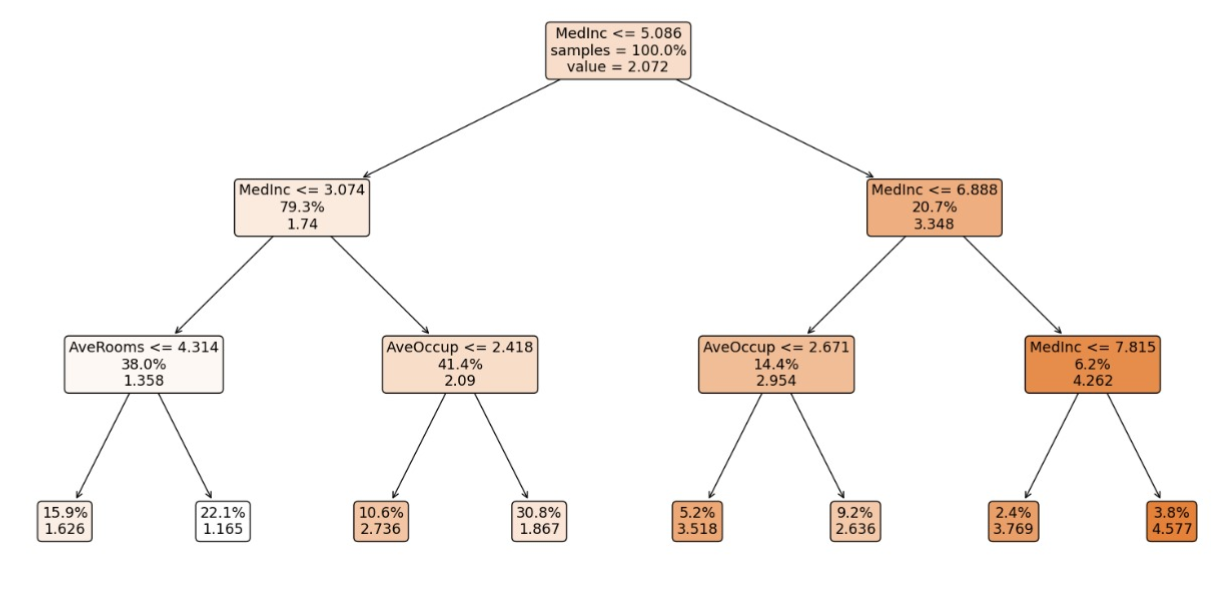
\includegraphics[width=1\textwidth]{figures/marco-teorico/tree-ilustrativo.png}
\caption{Árbol de decisión de ejemplo para predecir el precio de casas en miles de USD.}
\end{figure}
\label{figure1}

Entonces, observando el camino hasta el primer nodo hoja de la izquierda, en una zona donde el ingreso promedio es menor a $\text{\textdollar} 30740$ y la cantidad de habitaciones de las casas en promedio son menor a $4.3$, la predicción dada por el árbol es que en esa zona las casas en promedio cuestan $\text{\textdollar} 162600$.

Para determinar cuáles son las mejores divisiones para los nodos y darle un puntaje de qué tan bueno es un árbol de decisión existen distintos criterios. A lo largo de nuestro proyecto vamos a estar trabajando particularmente con problemas de regresión, es decir, dados ciertos datos, predecir un valor numérico, como el precio de un hogar. Debido a esto, utilizaremos como criterio el Error Cuadrático Medio (MSE por sus siglas en inglés), ya que es la alternativa más popular y extendida en la literatura e industria para este tipo de problemas. 

El MSE se define como el promedio de las diferencias entre las predicciones ($\hat{y_{i}}$) y los valores reales ($y_{i}$), elevadas al cuadrado:
\[
MSE = \frac{1}{n} \sum_{i=1}^{n} (y_{i} - \hat{y_{i}})^2 \,,
\]

con $n$ siendo la cantidad de datos observados.

Este criterio se utiliza para evaluar todos las posibles separaciones de datos con las características dadas (conocidas como \textit{features}). Aquella división que menor MSE da en cada paso es la división que se selecciona. Así sucesivamente hasta finalizar la construcción del árbol, que puede tener distintas normas para finalizar, como puede ser una profundidad máxima o la cantidad mínima de observaciones que debe haber en cada nodo hoja, decididas por el usuario.


\section{Random Forest}

Random Forest (RF) es un algoritmo de aprendizaje supervisado de tipo \textit{ensamble} introducido por \cite{breimanRF}, el cual se ha establecido como una herramienta estándar en el área de \textit{machine learning} dada su robustez y versatilidad a largo de diferentes aplicaciones. Básicamente este algoritmo propone, en lugar de crear un único árbol de decisión con toda la información disponible en entrenamiento, la creación de varios árboles de decisión, cada uno formado a partir de distintos subconjuntos de datos removiendo observaciones de datos, como podría ser, en el ejemplo anterior, quitar la información de algunas casas.

El proceso de generar subconjuntos de datos seleccionando aleatoriamente es lo que se conoce como \textbf{Bootstrapping}. Para cada árbol, se elige un subgrupo de datos de entrenamiento con reposición, lo que implica que algunas observaciones pueden repetirse mientras que otras pueden no ser elegidas. Este método se realiza con el objetivo de que no todos los árboles aprendan las mismas divisiones o cortes, sino que tengan estructuras diversas, para llegar a respuestas que toman en cuenta distinta información que podría ser también muy valiosa.

El entrenamiento de múltiples árboles con subconjuntos de datos mediante Bootstrapping se denomina \textbf{Bagging} (Bootstrap aggregating). En este contexto, a los datos que no utilizó cada árbol durante su entrenamiento debido a este proceso se los llama \textit{Out-Of-Bag} (OOB). Random Forest además de no considerar ciertos datos en cada árbol, también elimina ciertas características (features, en inglés) de las observaciones, por ejemplo, entrenar algunos árboles sin la variable \texttt{MedInc}.

Luego de realizar este entrenamiento de todos los árboles, se considera que el modelo de Random Forest está entrenado y listo para recibir datos nuevos y dar predicciones. Para hacer esto, lo que hace es pasar cada observación por todos los árboles y \textit{promediar las predicciones que estos realizan}, para dar una respuesta final (una predicción para cada instancia nueva).

La utilidad de tomar la media de las predicciones de los árboles radica en la relación de dos conceptos muy importantes en los modelos de aprendizaje supervisado:

\begin{itemize}
    \item \textbf{Sesgo}: es el error de un modelo debido a sus suposiciones al aprender de los datos. Un alto sesgo es una mala señal pues significa que se aprendió muy poco de los datos de entrenamiento y el modelo no logra generalizar a nuevos datos. Llamamos a esto \textit{underfitting} (subajuste).
    \item \textbf{Varianza}: es la sensibilidad del modelo a pequeños cambios en los datos. Una alta varianza no es deseada ya que implica que se aprendió demasiado de los datos, sobre ajustando a ellos impidiendo que el modelo generalice para datos nuevos. Llamamos a esto \textit{overfitting} (sobreajuste).
\end{itemize}

El proceso de Bagging, sumado a limitar las variables predictoras, permite que al realizar el promedio de árboles no tan correlacionados se reduzca la varianza debido a que cada uno de ellos ve distintos subconjuntos de datos/features y aprende en teoría características diferentes. Al hacer esto, podemos permitirnos entrenar árboles más profundos sin tener el problema de ser muy sensible a pequeños cambios en los datos como sí lo tenemos al hacer un único árbol de decisión, lo que reduce el sesgo.

Finalmente, un último concepto necesario desarrollar sobre Random Forest son las posibles configuraciones del modelo. Como usuarios del algoritmo, podemos definir cuántos árboles queremos generar, su profundidad máxima, si queremos hacer bootstrapping con los datos o solo con las features, entre otros. Estas configuraciones, que determinan cómo se entrena el modelo, son conocidas como \textbf{hiperparámetros}. 

Más formalmente, llamamos hiperparámetros a aquellos valores que no se aprenden directamente del entrenamiento, si no que se establecen previamente a comenzar el mismo, y afectan su comportamiento.
Los más relevantes para nuestro trabajo, y sobre los cuales recapitularemos más adelante son los siguientes:

\begin{itemize}
    \item \textbf{n\_estimators}: Es el número de árboles del bosque.
    \item \textbf{max\_depth}: Es la profundidad máxima a la cual permitimos llegar a cada árbol del bosque. Actúa como un regularizador, es decir, busca impedir que se aprenda excesivamente de los datos de entrenamiento (lo que causaría overfitting).
    \item \textbf{max\_features}: Es la cantidad máxima de características de los datos (features) que se consideran en cada corte del árbol.
\end{itemize}

\section{Sabiduría de las masas}

Random Forest, y en general los algoritmos de ensamble de modelos, tienen un fuerte vínculo con un fenómeno social ampliamente estudiado conocido como “\textit{Wisdom of Crowds}” o “Sabiduría de las masas”, el cual sugiere que, en ciertos casos, grandes grupos de personas son colectivamente más sabias que individuos expertos cuando se trata de problemas de decisión y predicción. La idea central es que los puntos de vista de los individuos están por naturaleza sesgados, mientras que tomar el promedio del conocimiento de una multitud puede resultar en eliminar este sesgo o ruido y sorprendentemente producir precisiones más precisas y confiables, en contraposición a lo que se pensaba en un principio, que “juntar ignorancia trae más ignorancia”.

El ejemplo clásico es el presentado por Francis Galton en su estudio donde introduce este fenómeno. \cite{galtonFrancis} había acudido a una feria donde se le pidió a los participantes que adivinaran el peso de un buey. Las respuestas fueron muy diversas y probablemente algunas fueron disparatadas y, sin embargo, el promedio de las respuestas dio sorprendentemente cercano al peso real del animal.

Más adelante, Surowiecki retomaría este concepto de la mano de su libro \textit{The Wisdom of Crowds} en 2004, dónde formaliza el concepto y presenta casos de estudios, principalmente en economía y psicología, para ilustrar cómo la capacidad predictiva de una multitud supera a la de sus miembros individuales. Por su parte, \cite{mackeyMadnessCrowds} menciona que no todas las multitudes son sabias. Estos son los criterios clave distinguen a las multitudes sabias de las irracionales (\cite{surowieckiWisdomCrowdsWhy2004}):

\begin{itemize}
    \item \textit{Diversidad de opinión}: Cada persona posee información privada y diversa, incluso si solo es una interpretación de hechos conocidos.
    \item \textit{Independencia}: Las opiniones de las personas no están determinadas por las opiniones de quienes las rodean.
    \item \textit{Descentralización}: Las personas son capaces de especializarse y aprovechar el conocimiento local.
    \item \textit{Agregación}: Existe algún mecanismo para transformar los juicios individuales en una decisión colectiva.
\end{itemize}

Como se puede notar, los modelos de ensamble justamente buscan a través de los mecanismos descriptos anteriormente cumplir estas condiciones.

\section{Experimento y analogía con Random Forest}

El trabajo de \cite{galtonFrancis} y la posterior consolidación de este concepto de la mano de \cite{surowieckiWisdomCrowdsWhy2004} fueron el puntapié para muchísimos otros estudios, entre los cuales se encuentra la investigación que fundamenta la idea de este trabajo de experimentación. Las conclusiones observadas en \cite{navajasAggregatedKnowledge} surgen de un experimento llevado a cabo con una audiencia multitudinaria durante un evento TEDx en Buenos Aires, Argentina.

El experimento consistió en realizarle preguntas de cultura general a los participantes (ej. “¿Cuánto mide la Torre Eiffel?”). En primer lugar, los participantes recibieron ocho preguntas y anotaron sus respuestas sin discutirlas ni charlar con nadie en la sala (etapa i1). Una vez hecho esto, se le pidió a la audiencia que se organizara y se dividiera en grupos de cinco integrantes de acuerdo al código numérico de sus hojas de respuesta. Se les volvió a otorgar cuatro de las ocho preguntas originales y se les dio un minuto para discutir sobre las preguntas y llegar a una nueva respuesta consensuada (etapa c). Finalmente, los participantes volvieron a responder las ocho preguntas iniciales por su cuenta, permitiéndoles revisar sus respuestas posterior al debate y cambiar su opinión (etapa i2). Además, cada participante reportó su nivel de confianza en las respuestas en una escala del $0$ al $10$.

Con las respuestas obtenidas, pudieron observar que la media de las predicciones consensuadas entre los integrantes de los grupos pequeños obtuvo una precisión mayor que la media de las predicciones individuales del grupo masivo. De esta forma, demostraron que promediando decisiones deliberadas y consensuadas en pequeños grupos es sustancialmente más preciso que la agregación de opiniones iniciales independientes.

Este resultado es justamente el que nos permite, trazando una analogía entre este experimento y el modelo de aprendizaje supervisado de Random Forest, plantear la hipótesis de este trabajo de investigación y experimentación descripta anteriormente. En cuanto a esta analogía entre experimentos, es oportuno profundizar sobre sus supuestos para comprender las decisiones tomadas a lo largo de este proyecto con el objetivo de mantener de la forma más fiel posible la correspondencia entre los experimentos.

Dentro de esta semejanza entre los experimentos, el primer elemento que podemos notar es el participante de la audiencia de TEDx que, en base a su conocimiento, sus experiencias, supuestos, preconceptos y sesgos, realizó algún tipo de razonamiento ya sea más o menos profundo para responder cada una de las preguntas, es decir, sus predicciones individuales e independientes. Aquí se puede notar entonces que podemos tomar al árbol de decisión como análogo, el cual en base a las observaciones que tuvo durante entrenamiento, su “experiencia”, construyó su estructura que marcará el proceso de decisión para cada una de las instancias a predecir, las “preguntas”.

Es decir, para la pregunta “¿Cuánto mide la Torre Eiffel?”, los participantes del experimento respondieron probablemente en base a su conocimiento sobre otros edificios o monumentos. Por su parte, para el caso de los árboles de decisión, si fue entrenado para predecir la altura de diferentes construcciones, por ejemplo, al recibir una instancia a predecir con características como su ubicación, el material con el que está construido y el año de inicio y finalización de la construcción, va a predecir la altura a partir de su estructura conformada por los datos observados en entrenamiento para la pregunta del estilo “¿Cuál es la altura de la construcción ubicada en París, con su principal material el hierro y que comenzó a construirse en 1887 y finalizó en 1889?”.

Notada la analogía entre los participantes humanos y los árboles de decisión, el siguiente paso natural y sencillo de observar es que así como se propone, con el concepto de inteligencia colectiva, tomar la media de las predicciones de los individuos, Random Forest realiza lo mismo pero con las predicciones de los árboles. De esa forma, así como se descubrió que la deliberación en grupos de individuos mejoró la precisión de las predicciones, en este trabajo se propone el desafío de experimentar mecanismos que simulen esta etapa intermedia de debate pero entre los \textit{árboles de decisión}.

\section{Metodologías de desarrollo y herramientas utilizadas}

Para comprender las decisiones tomadas y explicadas a lo largo del informe, es útil también comprender las metodologías de desarrollo implementadas, así como las herramientas utilizadas.
Para nuestras implementaciones, seleccionamos el lenguaje de programación \textbf{Python}, muy utilizado para este tipo de algoritmos de machine learning, el cual cuenta con una librería open-source con implementaciones de los mismos, llamada \textbf{Scikit-learn}. Modificando ese código de software abierto es que logramos poner en funcionamiento nuestros experimentos para incluir el mencionado ``debate'' entre árboles de decisión.

Para implementar estas experimentaciones, es necesario seguir las buenas prácticas definidas por los desarrolladores del código abierto de Scikit-learn. El principal fundamento de estas prácticas es el hacer uso de la \textbf{herencia de clases}. Para entender este enfoque, es fundamental conocer qué son las \textit{clases} y la \textit{herencia} en la programación orientada a objetos.

Una clase es un esquema o estructura que define un conjunto de atributos (datos) y métodos (funciones) que operan sobre esos datos. En otras palabras, es un modelo que permite crear objetos con características y comportamientos específicos. En el caso de Scikit-learn, las clases representan modelos de aprendizaje automático, el de un árbol de decisión para regresión por ejemplo es \texttt{DecisionTreeRegressor}, que contiene métodos para ajustar (\texttt{fit}) el modelo a los datos y realizar predicciones (\texttt{predict}) sobre datos nuevos.

Por su parte, la herencia es un mecanismo que permite crear una nueva clase a partir de una clase existente. La clase que se crea, conocida como \textit{subclase} o clase hija, hereda todos los atributos y métodos de la clase original, llamada \textit{superclase} o clase padre. Esto facilita la reutilización del código y permite extender o modificar funcionalidades sin tener que escribir el código desde cero. Por ejemplo, para implementar un algoritmo personalizado que aproveche las optimizaciones del \texttt{DecisionTreeRegressor}, podemos crear una subclase que herede de esta y modificar o añadir funcionalidades específicas para nuestro objetivo.

En el contexto de Scikit-learn, realizar la herencia de clases no sólo nos permite cumplir con las buenas prácticas sino que también nos permite mantener la compatibilidad con el resto del ecosistema de la librería y aprovechar sus ventajas como optimizaciones ya implementadas en el algoritmo, o utilizar métodos útiles como el que nos permite graficar árboles de decisión. Algunas de estas funciones están implementadas en \textbf{Cython}, un lenguaje que mantiene mucha de la sintaxis de Python pero suma la posibilidad de incluir código en C++, un lenguaje de más bajo nivel que Python el cual permite mejorar el rendimiento de las implementaciones.

Finalmente, utilizamos muchas otras librerías de código abierto, como Matplotlib para realizar nuestras visualizaciones, o Pandas para la manipulación de datos, entre otras, que incluyen todas aquellas que Scikit-learn necesita para funcionar (dependencias), como pueden ser NumPy o SciPy. Para su instalación, utilizamos un entorno virtual, una herramienta que permite instalar bibliotecas y dependencias como las mencionadas, sin afectar el sistema global u otros proyectos. El proceso de creación del mismo se encuentra detallado en la sección \hyperref[confi-entorno]{\textit{Configuración del Entorno}} del Marco Metodológico.

Para realizar modificaciones en el código como equipo y poder trabajar juntos en los mismos archivos, utilizamos \textbf{Github}, una plataforma en la nube que permite alojar y gestionar repositorios de Git para proyectos de software. Tiene incluido un sistema de control de versiones, que nos permitió en todo momento colaborar sin sobrescribir cambios y volver a antiguas versiones en caso de haber cometido errores. Nuestro repositorio, con todo el historial de cambios y el código para la versión finalizada del proyecto se puede encontrar \textcolor{blue}{\href{https://github.com/fedeegiorgi/proyecto-final}{aqui}}.

Por otra parte, a lo largo del proyecto utilizamos distintas herramientas dentro de las metodologías \textbf{Agile} para organizar nuestro trabajo ayudándonos a tomar mejores decisiones en base estimación de alcances y tiempos, como pueden ser:

\begin{itemize}
    \item \textbf{Sprints}: Los sprints son marcos de tiempo específicos, en general cortos en los cuales se realizan una serie de tareas ya previamente definidas, orientadas a alcanzar objetivos concretos y más pequeños dentro del proyecto. En nuestro caso, definimos ocho sprints, de dos semanas cada uno, donde definimos tareas con fechas y encargados designados con el fin de ir alcanzando importantes metas con el transcurso del tiempo. Estas tareas, siguiendo la filosofía agile, son modificadas según contratiempos, cambios de prioridades, etc.
    
    \item \textbf{Roadmap}: El roadmap, llamado en español hoja de ruta, es una herramienta que sirve para proyectar los objetivos principales de un proyecto a largo plazo, definiendo fechas esperadas para los mismos y como guía de la estructura del desarrollo de un proyecto. En el desarrollo de nuestro proyecto en particular, sirvió como una proyección que nos permitió ver nuestro progreso con el paso de los sprints, y adaptarlo en consecuencia. Tener estos hitos importantes proyectados fue de gran utilidad a la hora de definir prioridades. 
    \begin{itemize}
        \item Para su visualización utilizamos diagramas de gantt, una herramienta que permite comprender tanto el tiempo estimado para cada uno de los objetivos principales, así como las dependencias entre ellos, representándolos como barras en un eje temporal.
    \end{itemize}

\end{itemize}

Para el uso de estas herramientas utilizamos las plataformas Notion y ClickUp, que poseen funciones para la implementación de las mismas de manera sencilla.
% called by main.tex
%
\chapter{Marco Metodológico}
\label{ch::capitulo6}

Este capítulo tiene como objetivo detallar exhaustivamente la metodología llevada a lo largo de este trabajo de investigación con el fin de entender las decisiones y los pasos tomados para cumplir con los objetivos específicos del proyecto. A su vez, la documentación descripta a continuación servirá como base detallada para que los experimentos llevados a cabo puedan ser, en caso de ser necesario, reproducibles por terceros.

\section{Elección de datos de entrenamiento}

Como parte del objetivo de mantener la correspondencia entre el experimento de \cite{navajasAggregatedKnowledge} y el llevado a cabo en este proyecto, uno de los requisitos es asegurarnos que las predicciones de los árboles de decisión sobre el conjunto de datos de entrenamiento sigan una distribución parecida a la distribución de las respuestas de los participantes del experimento llevado en TEDx. De esta forma, siguiendo la analogía entre predicciones de árboles de decisión y estimaciones de individuos, nos aseguramos que la experimentación de nuevos mecanismos de agregación en Random Forest parte de la misma base que la experimentación en humanos.

Además, otro de los requisitos de los datasets a elegir es que sean adecuados para problemas de regresión, es decir que la variable a predecir sea continua y, a su vez, que haya diversidad entre los datasets en términos de cantidad y tipos (numéricos y categóricos) de atributos y de cantidad de observaciones. Por su parte, debíamos definir si aceptaríamos conjunto de datos con información faltante (missings) o no. Para cumplir estos requisitos fue necesario seguir un cuidado procedimiento para la elección de nuestros conjuntos de datos a utilizar en la evaluación de las alternativas.

En primer lugar, nos propusimos analizar los datos recolectados de las respuestas del experimento original. Para llevar a cabo este análisis, comenzamos solicitándole a los autores de la investigación los datos recolectados. Si bien en el experimento llevado a cabo en el evento en vivo TEDx se tomó un muestra muy grande de personas (N=5800), para el análisis posterior se decidió conservar aquellos datos correspondientes a los individuos y grupos que tenían toda la información completa (m=280 grupos, n=1400 individuos). Los autores nos compartieron efectivamente los datos filtrados y procesados.

Teniendo en cuenta que los datos tenidos en cuenta en la experimentación fueron aquellos que tenían toda la información completa, tomamos la decisión que los conjuntos de datos a seleccionar para el entrenamiento de nuestros modelos también tengan toda la información completa. 

Una vez obtenido los datos, en formato .MAT, procedimos a transformarlos en datos manejables con Python, como vectores de Numpy y archivos CSV. Dado que en el experimento, durante la segunda etapa donde ocurrían las decisiones colectivas, sólo se tenían en cuenta cuatro de las ocho preguntas que respondieron individualmente los participantes, decidimos enfocarnos en analizar la distribución sólo de las preguntas debatidas. Estas son:

\begin{itemize}
    \item ¿Cuántos goles se marcaron en la Copa Mundial de la FIFA 2010?,
    \item ¿Cuántas veces aparece la palabra “alegría” en la letra de la canción “Y dale alegría a mi corazón”?,
    \item ¿Cuál es la suma de todos los números en una ruleta?,
    \item ¿Cuánto costaba un barril de petróleo en 1970 (en centavos de dólar estadounidense)?
\end{itemize}

El primer acercamiento a los datos, como suele ser de costumbre, fue a través de realizar histogramas que nos permitan tener una primera intuición sobre la distribución de las respuestas para cada una de las preguntas del experimento. A simple vista pudimos notar que las respuestas de las cuatro preguntas seguían una distribución cercana a la forma típica de la distribución \textbf{log-normal}. 

Para confirmar esta suposición, procedimos a computar funciones de densidad log-normales ajustadas según las estimaciones de sus parámetros sobre los datos. Para ello, utilizamos la librería \texttt{scipy.stats} que permite estimar en base a los datos los parámetros:

\begin{itemize}
    \item \texttt{shape}: desvío estándar $\sigma$.
    \item \texttt{loc}: parámetro de locación sobre el eje $x$
    \item \texttt{scale}: $e^{\mu}$, mediana de la distribución.
\end{itemize}

Con estos parámetros estimados, se pueden graficar las curvas de densidad para luego contrastar con las funciones de densidad observadas empíricamente en los datos de la experimentación de Navajas\footnote{Figuras en \hyperref[appendix1]{Apéndice 1}.}. Observando las figuras vimos que, para el tipo de precisión que necesitamos, la semejanza visualmente es suficiente.

Identificada la distribución de la experimentación de \cite{navajasAggregatedKnowledge}, el siguiente paso era preparar el procedimiento que seguiríamos para evaluar datasets y determinar cuáles cumplen los requisitos de distribución. Para ello, entendimos que deberíamos tener un soporte analítico dado que no sería posible evaluarlos de manera visual. Esto se debe a que, recordando la analogía entre una fila u observación de un dataset con una pregunta, habría que analizar las distribuciones de predicciones de los árboles para cada una de las instancias de validación luego de haberse entrenado. Es sencillo notar que para datasets con miles de instancias de validación, como las que apuntamos, observar la distribución para cada una de ellas de manera visual es inviable.

Como soporte analítico para comprobar si las funciones de densidad siguen la distribución esperada, decidimos utilizar test de hipótesis ya implementados. Para comprobar la distribución log-normal aprendimos que se suele utilizar el test \textbf{Kolmogorov-Smirnov} por lo que decidimos tomar la implementación de \texttt{scipy.stats} en Python y probarlos con los datos del experimento de Navajas. Observando los resultados, vimos que el p-valor era demasiado chico, muy por debajo de $0.05$ lo cuál indicaría que debemos rechazar la hipótesis nula $H_0$ (que la distribución de los datos siguen una distribución log-normal), lo cuál se contrapone con nuestra interpretación visual. 

Profundizando en la investigación de este test de hipótesis, entendimos que el mismo es demasiado exigente para el tipo de búsqueda que estábamos realizando. Por ese motivo, decidimos seguir con otra alternativa. Esta consistió en aplicar una transformación logarítmica a los datos, con el supuesto que haciendo esto, obtendríamos que los datos transformados sigan una distribución normal. Efectivamente, esto fue lo que sucedió comprobándolo de manera visual siguiendo el mismo procedimiento utilizado anteriormente con la distribución log-normal\footnote{Figuras en \hyperref[appendix2]{Apéndice 2}.}.

Además de comprobarlo gráficamente, aplicamos un test de hipótesis, en este caso el \textbf{Shapiro-Wilk}, que mide si muestras siguen una distribución normal. En este caso, si bien ocurrió lo mismo con el p-valor como con Kolmogorov-Smirnov, en este caso los valores del estadístico del test se aproximaban mucho a 1, lo que indica que la distribución se encuentra muy cercana a la distribución normal \footnote{Tabla en \hyperref[appendix3]{Apéndice 3}.}. Vemos que el promedio de este estadístico para las cuatro preguntas es $0.9809$.

Completado el análisis sobre los datos del experimento, creamos un código en Python que dado un dataset:

\begin{enumerate}
    \item Se divide entre conjunto de entrenamiento y validación.
    \item Se entrena un modelo de Random Forest tradicional con el conjunto de entrenamiento con 100 árboles de decisión.
    \item Por cada instancia de validación se toman las predicciones de los 100 árboles de decisión, se le aplican una transformación logarítmica para luego aplicarles el test de hipótesis de Shapiro-Wilk.
    \begin{enumerate}
        \item En caso de que el valor del estadístico resultante esté en el rango de un $\pm 10\%$ del promedio del estadístico sobre los datos de Navajas ($0.9809$) se toma como caso favorable.
        \item Caso contrario, se toma esa instancia como no favorable.
    \end{enumerate}
    \item Se computa el porcentaje de instancias favorables sobre la totalidad, para obtener nuestro porcentaje de aceptación de un dataset.
\end{enumerate}

Analizados unos 30 datasets de fuentes como \textit{OpenML} y \textit{Kaggle}, fuimos generando un ranking de los mismos en base al porcentaje de aceptación computado\footnote{Tabla en \hyperref[appendix4]{Apéndice 4}.}. Observando los resultados, decidimos tomar como datasets principales para la experimentación \textit{House 8L}, \textit{Wind Speed} y \textit{Carbon Footprint} dado que están entre aquellos con mayor porcentaje de aceptación de distribución. Además, entre los datasets seleccionados, hay diversidad en cantidad de instancias y cantidad de \textit{features} (columnas). En el caso de \textit{House 8L}, se predice el precio de una casa basado en características numéricas exclusivamente, mientras que en \textit{Wind Speed}, se predice la velocidad del viento a partir de variables como precipitación, temperatura y fecha. Por su parte, en \textit{Carbon Footprint}, se estima la emisión de carbono de individuos basada en sus consumos de energía e insumos, como que tipo de transporte utiliza y la cantidad de ropa nueva comprada al mes.

Una vez seleccionados los principales conjuntos de entrenamiento, procedimos a analizar con mayor profundidad su conformación\footnote{Fuente de los datasets en \hyperref[appendix5]{Apéndice 5}.} y realizar ingeniería de atributos en las columnas necesarias de cada uno de ellos:

\begin{itemize}
    \item \textit{House 8L}: Este conjunto de datos no requirió modificaciones, ya que todas sus columnas son numéricas y no identificamos la necesidad de realizar transformaciones.
    \item \textit{Wind Speed}: Este dataset contiene una columna llamada \texttt{DATE}, donde las fechas están formateadas como Año-Mes-Día. Para simplificar el análisis y reducir la cantidad de columnas generadas mediante técnicas como \textit{One-Hot Encoding} (OHE), desglosamos esta columna en tres nuevas: \texttt{Year}, \texttt{Month} y \texttt{Day}.
    \item \textit{Carbon Footprint}: Este conjunto de datos presentaba dos columnas que requerían transformaciones: \texttt{Recycling} y \texttt{Cooking\_With}. Por ejemplo, la columna \texttt{Cooking\_With} contenía listas de valores como \texttt{["Microwave", "Grill", ``Airfryer'']}. Para facilitar su análisis, creamos columnas binarias para cada elemento de las listas, resultando en nuevas columnas como \texttt{Cooking\_With\_Microwave}, \texttt{Cooking\_With\_Grill} y \texttt{Cooking\_With\_Airfryer}. Aplicamos el mismo enfoque a la columna \texttt{Recycling}.
\end{itemize}

A su vez, además de estos 3 conjuntos de entrenamiento, decidimos tomar tres conjuntos más que tenían un porcentaje de aceptación más bajo sobre la distribución. De esta forma, con los mismos podríamos evaluar también si la distribución log-normal de las predicciones iniciales de los árboles de decisión es un factor determinante para las modificaciones o no. Entre estos datasets adicionales se encuentra \textit{Abalone}, conjunto de datos utilizado en \cite{breimanRF}, \textit{Rainfall} y \textit{Flight price}.


\section{Configuración del entorno}
\label{confi-entorno}

Como mencionamos previamente en el marco teórico, utilizamos un entorno virtual para instalar todas las herramientas necesarias a lo largo del proyecto con dos objetivos principales. En primer lugar, evitar problemas de compatibilidad entre las distintas herramientas y, por otro lado, asegurarnos de que cada una de las computadoras utilizadas para el proyecto tenga exactamente la misma configuración.

Dentro del entorno, instalamos la versión editable de Scikit-Learn, descargando su versión \texttt{1.6.dev0} el día 19 de agosto del 2024, y partimos de esa versión para realizar todos nuestros cambios, asegurando que ninguna actualización nos cause problemas y que los experimentos sean bajo las mismas condiciones. Esta versión editable, además, nos permitió probar de manera muy sencilla nuestros cambios, ya que está preparada para reflejar inmediatamente cualquier cambio hecho al código de la biblioteca sin necesidad de realizar ningún tipo de re-instalación.

El paso por paso para configurar este entorno, ya sea desde una computadora Linux o Windows se puede encontrar en el \hyperref[appendix6]{Apéndice 6}.

\section{Decisiones implementativas}

Con respecto a la implementación de los experimentos, para cumplir con las buenas prácticas de la librería \textit{Scikit-Learn} y buscar mantener el código original sin modificaciones, optamos por usar herencia de clases por los motivos anteriormente descriptos en el Marco Teórico.

En primer lugar, identificamos, dentro de la totalidad de la librería, que para nuestro proceso de experimentación debíamos utilizar como base la clase \textbf{\texttt{RandomForestRegressor}} que implementa el algoritmo de Random Forest original. A partir de allí, entendimos que todas nuestras alternativas de RF iban a tener en común el proceso de agrupamiento de los árboles para la posterior “deliberación” entre los mismos.

Con ese supuesto, decidimos implementar la clase \textbf{\texttt{RandomForestGroupDebate}}, la cuál hereda de \texttt{RandomForestRegressor}. La misma agrega a la implementación original la funcionalidad de poder agrupar tanto los árboles de decisión en sí (método \texttt{group\_split()}), como las predicciones independientes de los mismos (método \texttt{group\_split\_predictions(predictions)}). Ambos métodos dividen el conjunto de árboles en subgrupos, controlados por el nuevo parámetro de los modelos: \texttt{group\_size} (tamaño de los grupos).

Una vez definida esta clase “base”, las distintas variantes del modelo que buscan simular el “debate” entre árboles heredan \texttt{RandomForestGroupDebate} para ya tener incorporada la funcionalidad de agrupamiento, sin necesidad de re-implementarla. Es así como las nuevas clases cuentan con adaptaciones o re-implementaciones de los dos métodos fundamentales, \texttt{fit} y \texttt{predict}, de acuerdo a los distintos enfoques de simulación de la deliberación. 

Además, reutilizamos la función de paralelización de predicciones de árboles de la implementación original, la cuál aporta como mecanismo para hacer más eficiente el cómputo de las predicción sobre nuevos datos. Para algunas de las implementaciones de alternativas, realizamos un ajuste sobre la misma. En lugar de acumular las predicciones en una suma, la función se modificó para almacenarlas individualmente.

\section{Modelos de simulación del debate}

En esta sección se detallan las diferentes alternativas al RF exploradas e implementadas que incorporan etapas intermedias entre las predicciones de los árboles de decisión y su agregación, buscando imitar y simular la deliberación y búsqueda de predicciones consensuadas dentro de los grupos.

\subsection{Exclusión de extremos}

En esta alternativa exploramos la idea de simular la exclusión de “opiniones extremas” dentro de un debate para así evaluar si esto mejora la predicción colectiva del grupo y crea un consenso más equilibrado y menos variable.  Esta idea surge del supuesto de que probablemente durante el debate entre personas, si hay un consenso de que algunas predicciones individuales están muy alejadas de la mayoría, aquellas más extremas serán excluidas de la predicción final. 

En primer lugar, nos pareció oportuno utilizar método de exclusión de valores atípicos (\textit{outliers}) con el \textit{Rango Intercuartil} (Interquartile Range o IQR en inglés). Este método tiene un extendido uso en el área de estadística y análisis de datos, popular  por su uso para los gráficos de boxplots.

Para ello, ideamos el modelo \textbf{\texttt{IQRRandomForestRegressor}}. El mismo, se implementa mediante una clase con el mismo nombre que sobrescribe el método \texttt{predict} de \texttt{RandomForestRegressor} para poder filtrar valores extremos en las predicciones individuales de los árboles. Para hacerlo, en primer lugar, se calcula el IQR de las predicciones individuales de los árboles en cada grupo usando el primer cuartil (Q1) y el tercer cuartil (Q3), donde:
\[
IQR = Q3 - Q1
\]

Luego, se descartan las predicciones que se encuentren fuera del rango de aceptación, definido como:
\[
[Q1 - 1.5 \cdot IQR, Q3 + 1.5 \cdot IQR]
\]

Una vez obtenidas las predicciones aceptadas, se computa la media de las predicciones que quedaron en cada grupo para así conformar la predicción del grupo. Finalmente, se promedian los resultados de todos los grupos para obtener la predicción final del modelo \texttt{IQRRandomForestRegressor}.

En segundo lugar, como otra alternativa de exclusión que permita explorar rangos definidos por el mismo usuario, ideamos el modelo \textbf{\texttt{PercentileTrimmingRandomForestRegressor}}. El mismo fue implementado con una clase que sobrescribe la función \texttt{predict} de la clase original para también filtrar las predicciones extremas de los árboles pero utilizando percentiles variables.

Para ello, cuenta con un hiperparámetro llamado \texttt{percentile}. El mismo funciona de manera tal que si, por ejemplo $percentile = 2$, entonces $p_{inf}$ (el percentil inferior) es el número que deja un $2\%$ de los datos a izquierda y $p_{sup}$ (el percentil superior) el que lo hace a derecha.

En en este algoritmo entonces, para cada grupo de predicciones, se calculan los percentiles inferior y superior ($p_{inf}$ y $p_{sup}$), definidos por el mencionado hiperparámetro y una vez calculados dichos valores, se eliminan las predicciones fuera del rango:
\[
[p_{inf}, p_{sup}]
\]

Finalmente, al igual que en IQR, se calcula el promedio de las predicciones aceptadas de cada grupo y se obtiene la predicción final promediando todos los grupos.

Es importante notar que IQR y Percentile Trimming son métodos distintos. IQR calcula límites \textbf{dinámicos} basados en la dispersión de los datos (Q1 y Q3), mientras que Percentile Trimming utiliza percentiles \textbf{fijos} definidos por el usuario. Además, Percentile Trimming siempre elimina valores extremos, mientras que IQR podría no hacerlo si todas las predicciones se encuentran dentro del rango calculado. Por estas razones, no existe un valor de percentil que coincida exactamente con los límites del IQR.

\subsection{Media ponderada por confianza}

Este enfoque busca simular un debate en el que cada participante tiene un peso proporcional al nivel de confianza en sus argumentos para conformar la predicción consensuada grupal. Es así como, aquellos árboles con un mayor nivel de confianza, determinada por su historial de predicciones correctas, influyen más en la decisión grupal.

Este concepto fue ejecutado mediante el modelo \textbf{\texttt{OOBRandomForestRegressor}}. El mismo, también implementado con una clase que hereda de \texttt{RandomForestRegressor}, sobrescribe el método \texttt{fit} para, además de construir los árboles de decisión independientes, calcular el \textit{nivel de confianza} de cada árbol.

Definimos la \textit{confianza} como la capacidad del árbol para predecir correctamente sobre aquellas muestras no seleccionadas durante el proceso de \textit{bootstrapping} y por lo tanto no utilizó para su entrenamiento. Estas observaciones del conjunto de entrenamiento son las ya mencionadas muestras \textit{Out-Of-Bag} (OOB), de aquí el nombre del modelo. Son estas observaciones las que serán evaluadas, como si fuesen el conjunto de validación, para medir la performance del árbol prediciendo mediante el error cuadrático medio (MSE). 

Esta performance, medida en MSE, será la base para la conformación del \textit{nivel de confianza} de cada árbol. Para ello, se le asigna a cada árbol un peso inverso de forma que los árboles con menor MSE tengan mayor peso. Así, quedan conformados como: 
\[
w_i = \frac{1}{MSE} \,\, \forall \,\, \mathrm{tree_i} \in \mathrm{Trees}.
\]

Finalmente, dentro de cada grupo, se normalizan dichos pesos de manera lineal para conformar la “confianza” como:
\[
c_i = \frac{w_i}{\sum_{j=0}^{s} w_j}\,, \; \text{donde} \,\, \mathrm{s = group\_size}.
\]

Por su parte, en el método \texttt{predict}, se buscan las predicciones de los árboles en cada grupo y con los índices de confianza calculados en \texttt{fit} se computa la media ponderada de las predicciones de los árboles en cada grupo como:
\[
\hat{Y} = \sum_{i=0}^{s} \, \hat{y}_i \cdot c_i
\]

Finalmente, como en todos los modelos, aplicamos la agregación simple de la media entre todas las predicciones de cada grupo.

Habiendo implementado esta alternativa, surgió de manera natural preguntarnos qué sucedería si combinamos esta idea de niveles de confianza de los árboles junto con la idea de exclusión de extremos para así, modelar una deliberación más compleja. De esta forma, surgió la ideación del modelo \textbf{\texttt{OOBPlusIQRRandomForestRegressor}} que combina las simulaciones implementadas en \texttt{IQRRandomForestRegressor} y \texttt{OOBRandomForestRegressor}.

En este modelo, se computan durante entrenamiento los pesos inversos $w_i$ de cada árbol con el MSE calculado sobre las instancias OOB. Pero, a diferencia de \texttt{OOBRandomForestRegressor}, los índices de confianza deberán determinarse en este caso durante predicción dado que se deben excluir de la normalización aquellos pesos de los árboles cuyas predicciones quedaron fuera del rango de IQR.

Entonces, el método \texttt{predict} se encargará en primer lugar de obtener y agrupar las predicciones iniciales de los árboles. Luego, al igual que en \texttt{IQRRandomForestRegressor} se descartan las predicciones consideras \textit{outliers} y, finalmente, se computan los índices de confianza sólo sobre aquellos árboles cuyas predicciones no fueron excluidas. Es así como, en este caso la predicción final del grupo estará dada por:
\[
\hat{Y} = \sum_{i=0}^{s} \hat{y}_i \cdot c_i \; \forall \; \hat{y}_i \in \mathrm{[Q1 - 1.5 \cdot IQR, Q3 + 1.5 \cdot IQR]}
\]

\subsection{Combinación de árboles}

La idea de combinar los árboles pertenecientes a cada grupo busca simular cómo, en algunos casos, la deliberación y búsqueda de respuestas consensuadas no pasa por simplemente combinar las predicciones individuales, sino que por el contrario, se buscan compartir los argumentos e ideas para conformar un nuevo razonamiento grupal.

Análogamente a pensar en partes pequeñas del razonamiento de los individuos, se pueden pensar a los cortes o divisiones de cada nivel de partición de los árboles de decisión como la unidad mínima en la que se puede dividir el “razonamiento” de la estructura de los árboles de decisión. A su vez, como se detalló en el marco teórico, la jerarquía de las particiones en los árboles de decisión siguen la lógica de que aquellas más cerca de la raíz del árbol son aquellas que más información aportan para la toma de decisión para la predicción final.

Con estas ideas en mente, surgió el modelo \textbf{\texttt{FirstSplitCombinerRandomForestRegressor}}, el cuál durante entrenamiento, una vez construidos los árboles iniciales independientes, se los agrupa y combina generando así un único árbol por grupo. Para conformar este árbol único, basándonos en la premisa de que los primeros cortes de cada árbol son los que contienen mayor información, se toman y almacenan cuáles fueron las columnas (\textit{features}) y valores de corte (\textit{thresholds}) de cada nodo raíz de los árboles del grupo. Con esta información es que se construirá un nuevo árbol representativo de “primeros cortes”, con el objetivo de aprovechar al máximo la información más significativa.

Para implementar esta alternativa, no solo requirió modificar los métodos \texttt{fit} y \texttt{predict}, sino también implementar un nuevo mecanismo de construcción de los árboles. Dado que la implementación original de construcción de árboles se encuentra en la sección de la librería implementada en Cython, decidimos también hacerlo en ese lenguaje y heredar la clase encargada originalmente de la construcción llamada \texttt{DepthFirstTreeBuilder}. En la nueva clase heredada, re-implementamos el método \texttt{build} para que ahora a partir de las \textit{features} y \textit{thresholds} de los primeros cortes de los árboles se construya un nuevo árbol.

Esta construcción está dada por tomar cada nodo raíz de los árboles iniciales y concatenarlos a lo largo de los niveles del nuevo árbol, así combinando las decisiones iniciales de cada árbol para conformar nuevos caminos de decisión. Es decir, el nodo raíz del nuevo árbol será, por ejemplo, el nodo raíz del primer árbol del grupo y sus nodos “hijos”, tanto a izquierda como a derecha, serán el nodo raíz del segundo árbol del grupo, y así sucesivamente. En la \hyperref[figure2]{Figura 2}, se puede observar un ejemplo ilustrativo de cómo quedará conformado un árbol combinado a partir de tres árboles iniciales. Se puede notar, como la profundidad de los nuevos árboles combinados estarán dados por el tamaño de los grupos conformados.

\begin{figure}[h]
\centering
    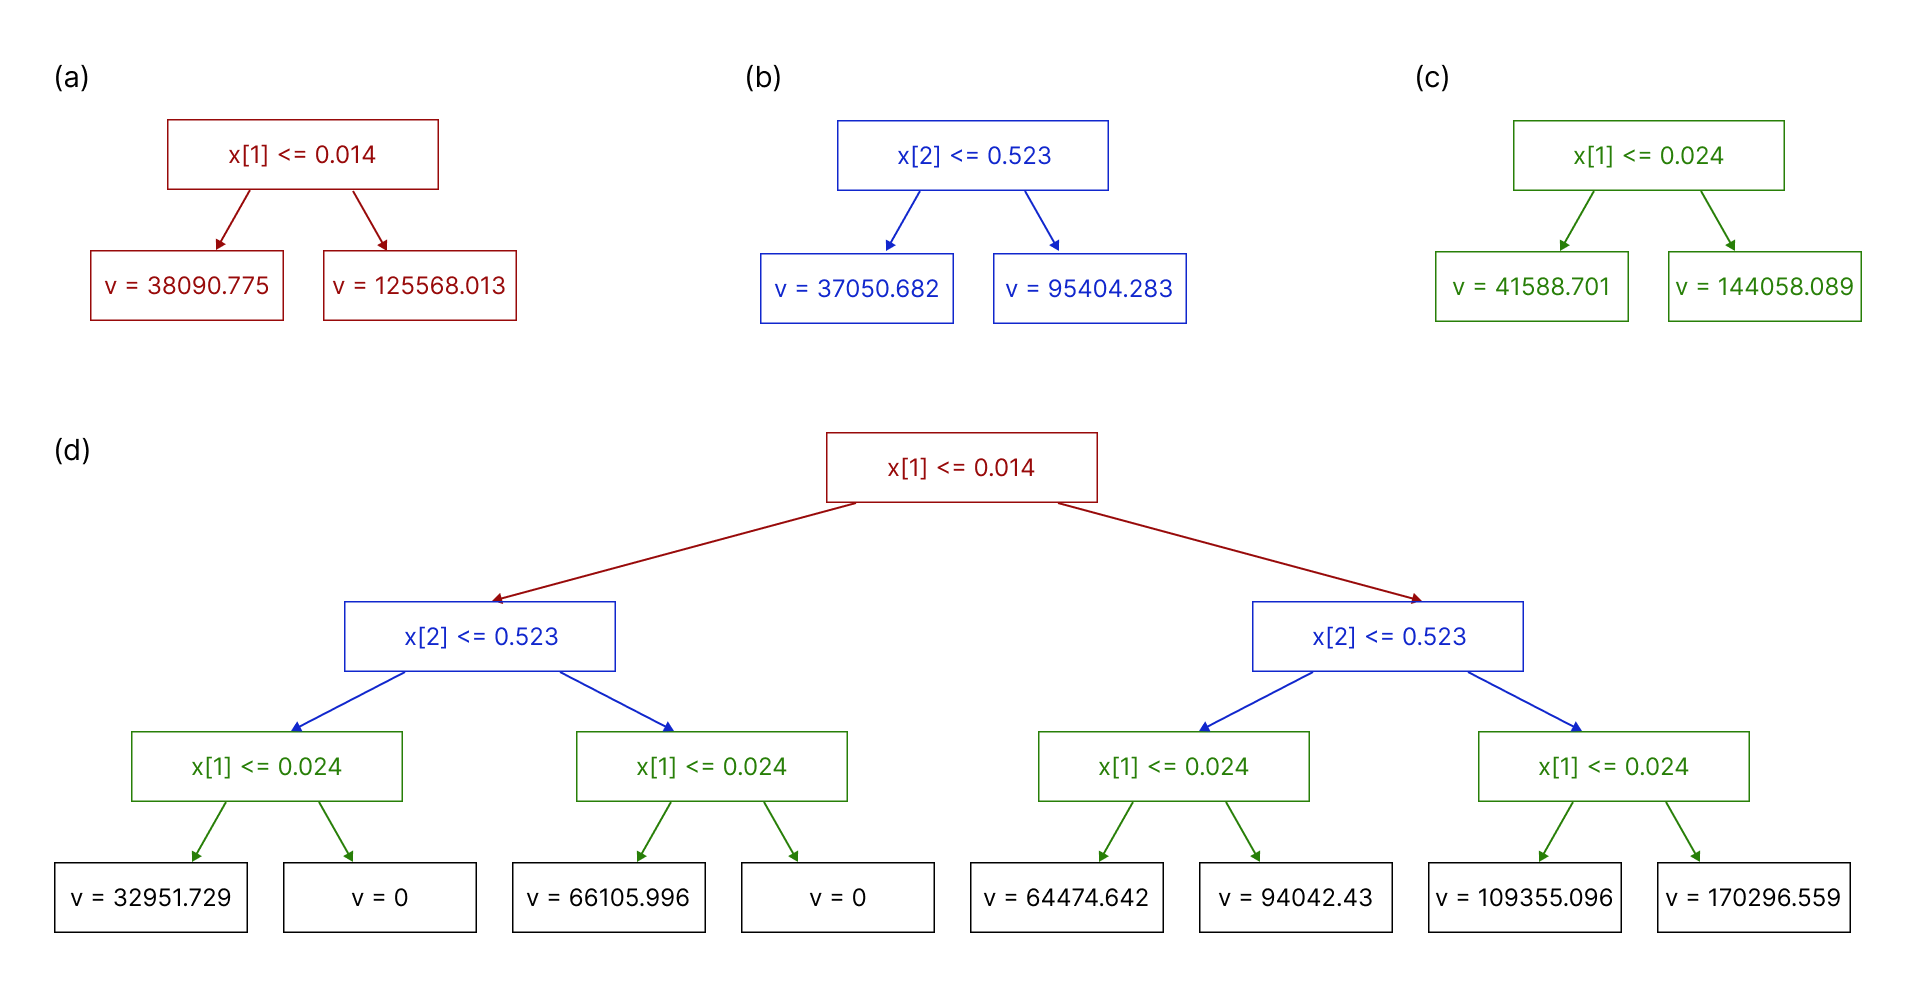
\includegraphics[width=1\textwidth]{figures/marco-metodologico/FSC.png}
\caption{Ejemplo ilustrativo de combinación de árboles dónde (a), (b) y (c) son los árboles iniciales y (d) es el combinado resultante.}
\end{figure}
\label{figure2}

Habiendo discutido el mecanismo de construcción de los nuevos árboles, entonces, el modelo \texttt{FirstSplitCombinerRandomForestRegressor} durante entrenamiento con el método \texttt{fit} se agrupan los árboles iniciales, obtiene la información relevante de los nodos raíz de cada uno de ellos y se ejecuta la construcción cada uno de los nuevos árboles de cada grupo con el nuevo constructor definido e implementado en Cython. Este constructor crea los nodos necesarios según la estructura de árboles de la librería y luego se computan los valores de las hojas según la unión de las muestras utilizadas por los árboles iniciales del grupo.

Una vez conformados los nuevos árboles en entrenamiento, al querer predecir sobre nuevas instancias se deberá llamar al método \texttt{predict} que, de forma paralela, computará la predicción de cada grupo para cada observación utilizando los árboles de primeros cortes combinados. Al igual que siempre, las predicciones de cada grupo serán promediadas para obtener la predicción final del modelo.

Este modelo tiene algunas particularidades implementativas que valen la pena resaltar. En primer lugar, dado que de los árboles de decisión iniciales sólo se toman los primeros cortes, nos pareció oportuno que al construirse, se hagan con una profundidad limitada de un sólo nivel. De esta forma se acelera mucho el proceso de cómputo del entrenamiento del modelo.

Por otro lado, cuando se realizan entrenamientos con grupos de más de 20 árboles (regulado por el hiperparámetro \texttt{group\_size}), el algoritmo sufre problemas de memoria, en particular el problema \textit{OOM Killer} (\textit{Out of Memory}), debido a la elevada cantidad de información se debe almacenar de los árboles iniciales. De todas formas, llevándolo nuevamente a la analogía, así como es muy difícil que muchas personas debatan y lleguen a un acuerdo, no nos parece que tenga sentido armar grupos de muchos árboles tampoco.

\subsection{Conocimiento compartido entre árboles}

En esta alternativa, buscamos emular cómo el intercambio de “conocimiento” entre individuos puede influir en sus decisiones. Los participantes ajustan sus argumentos tras intercambiar puntos de vista y recibir retroalimentación durante la deliberación, llevando a que tomen decisiones más informadas. Sin embargo, también es considerable pensar que los preconceptos más fuertes y arraigados sean más difícil de modificar, por lo que si bien el intercambio puede promover modificaciones en el razonamiento, las bases se sostienen.

Con estas hipótesis sobre el posible mecanismo por el cuál se comparte información entre pares, surge el último modelo experimentado llamado \textbf{\texttt{SharedKnowledgeRandomForestRegressor}}. La idea principal es que así como cada persona tiene ideas preconcebidas y al interactuar y compartir información con otros, tiene la posibilidad de incorporar nuevas perspectivas que pueden alterar su forma de pensar, esto mismo se puede llevar de cierta manera a los árboles de decisión mediante el control de la profundidad del árbol.

De esta forma, este modelo incorpora el hiperparámetro \texttt{initial\_max\_depth} que controla la profundidad de los árboles de decisión iniciales. Es decir, cada árbol comienza construyéndose de forma convencional con sus observaciones derivadas del mecanismo de \textit{bagging}. Sin embargo, alcanzado el nivel de profundidad \texttt{initial\_max\_depth}, se pausa la construcción del árbol. A partir de allí, los árboles iniciales se agrupan, como en los anteriores modelos, y se produce el intercambio de “información” que cada árbol tuvo en entrenamiento. Este intercambio consiste en que, para cada árbol del grupo, sus observaciones de entrenamiento se utilizan para que los otros árboles del grupo computen predicciones y se las comparten con el árbol en cuestión. De está forma, cada árbol sumará a sus datos de entrenamiento $group\_size - 1$ nuevas features (columnas) que podrá utilizar para continuar su entrenamiento.

A partir de la profundidad \texttt{initial\_max\_depth}, cada árbol continuará su entrenamiento con el algoritmo habitual pero contando con la posibilidad de usar las nuevas features como variables de corte para niveles del árbol más profundos. Conformados estos nuevos árboles extendidos se da por concluido el proceso de entrenamiento del modelo. En la \hyperref[figure3]{Figura 3} se puede ver un ejemplo de un árbol extendido y su correspondiente inicial entrenado sobre el dataset \textit{House\_8L} donde se resaltan los nodos dónde el corte se realiza sobre las variables correspondientes a las predicciones de los pares.

\begin{figure}[h]
\centering
    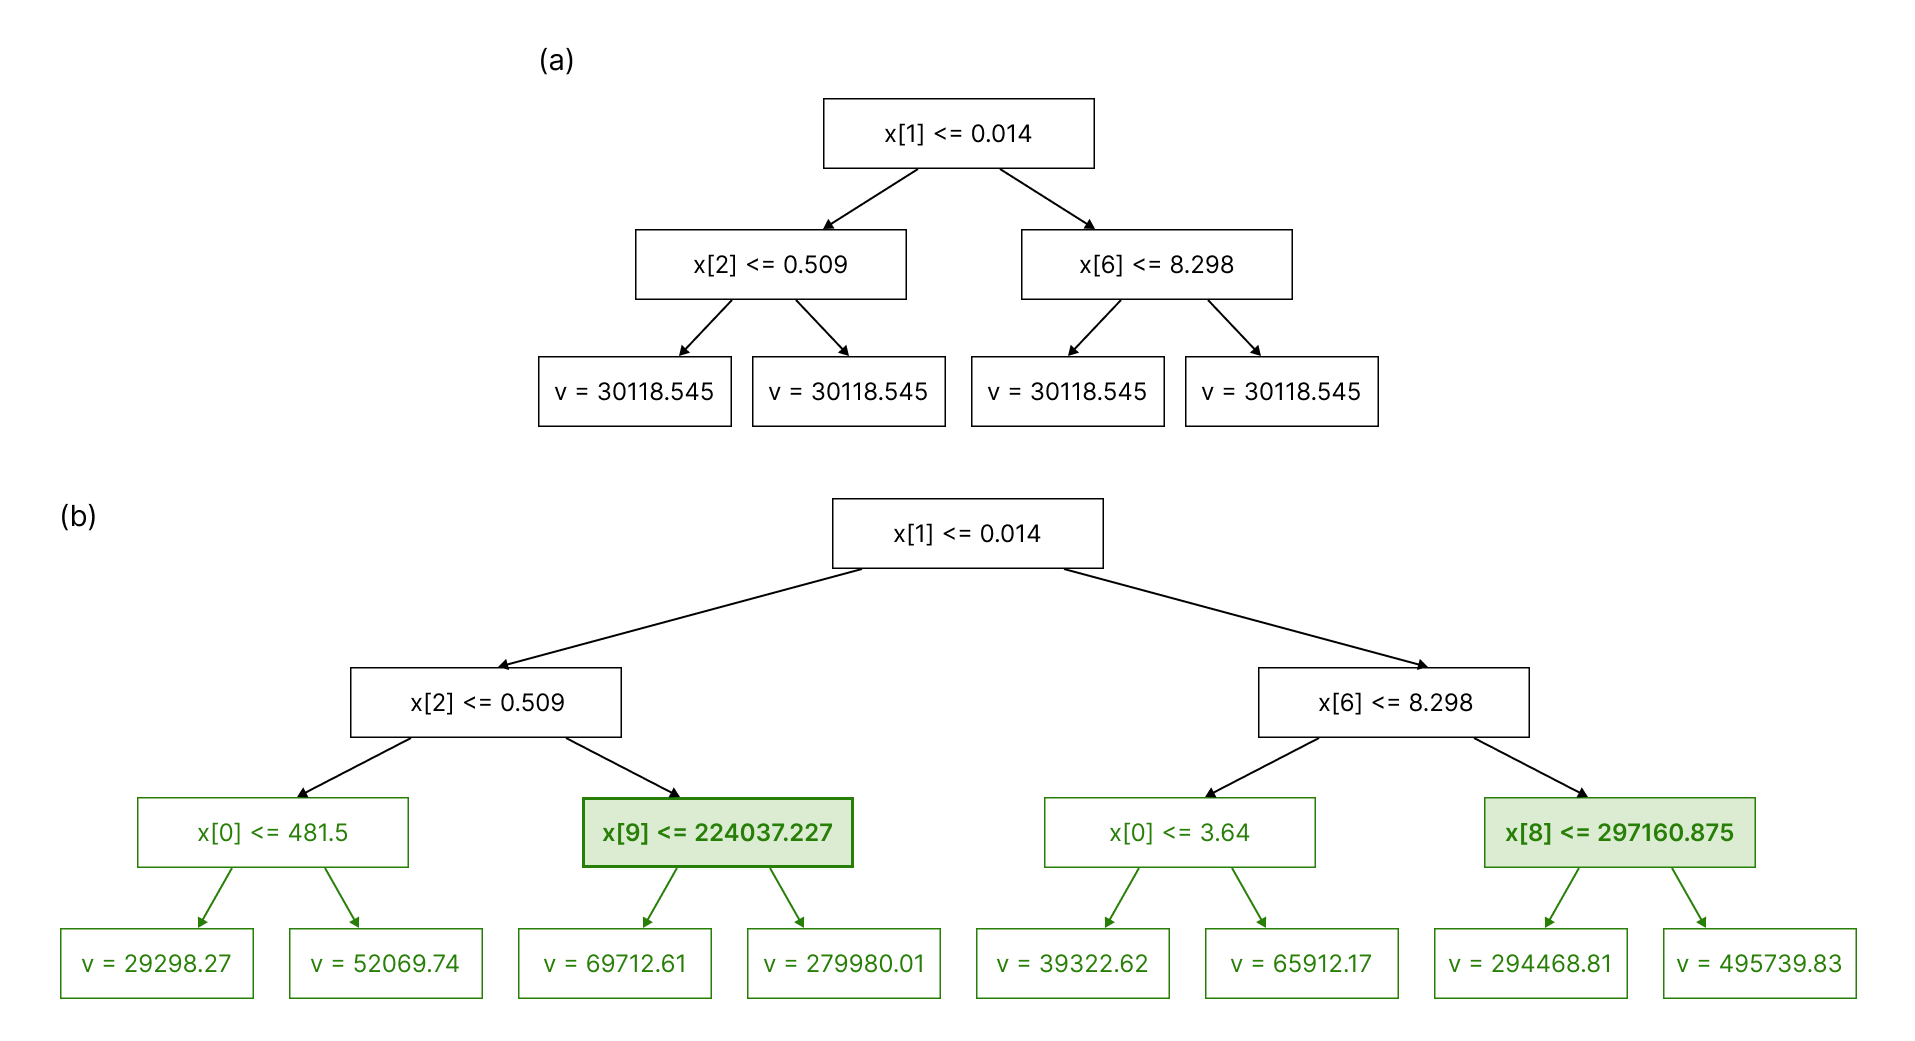
\includegraphics[width=1\textwidth]{figures/marco-metodologico/SK.png}
\caption{Árbol inicial (a) y extendido (b) entrenado sobre dataset House\_8L que tiene 8 features originales.}
\end{figure}
\label{figure3}

En cuanto a aspectos implementativos, esta alternativa fue la más desafiante. En un principio, la idea más natural era tomar toda la información de la estructura de los árboles iniciales para así, al crear los árboles extendidos, se fuerce el algoritmo a seguir la misma estructura que el árbol original hasta la profundidad  \texttt{initial\_max\_depth}. Sin embargo, eso conlleva el desafío de manejo memoria más minucioso. Es por ello que, luego de varias pruebas, surgió la idea que en el lugar de pasar la información original de los árboles, se construyan nuevos árboles con el algoritmo original pero limitando a que no se puedan utilizar las features provenientes del intercambio de información hasta alcanzar la \texttt{initial\_max\_depth}. Gracias a que tanto el entrenamiento original y extendido se realizan bajo la misma semilla, la correspondencia estre los mismos está garantizada.

Esta alternativa, no sólo es más eficiente en el uso de memoria, sino que también requiere menos modificaciones al algoritmo de construcción. En este caso tuvimos que implementar en Cython una nueva versión del \texttt{Splitter}, clase encargada de buscar los mejores cortes en cada paso de la construcción. La modificación centralmente limita las features disponibles hasta alcanzar el nivel dado por \texttt{initial\_max\_depth}, sacrificando ciertas optimizaciones del algoritmo con el fin de garantizar la correspondencia entre los árboles iniciales y sus extendidos.

En cuanto al método \texttt{predict} del modelo \texttt{SharedKnowledgeRandomForestRegressor}, es necesario notar ciertas particularidades. Para que nuevas muestras puedan atravesar los árboles de decisión extendidos, es necesario que cuenten con la misma cantidad de features que en entrenamiento. Es decir, así como durante entrenamiento cada árbol incorporó las predicciones de sus pares en su versión inicial, en predicción debe suceder lo mismo. Es así que para predecir nuevas observaciones, las mismas serán primero computadas por los árboles iniciales y esas predicciones se agregarán como features para ahora sí poder ser procesadas por los árboles extendidos.
Computadas las predicciones sobre cada árbol extendido, como en los restos de los modelos, se calcula la media dentro de cada grupo y luego se toma la media de los grupos para así conformar la predicción final del modelo.

\section{Optimización de hiperparámetros}

Una vez que los modelos con modificaciones al RF definidos, implementados y listos para ejecutarse, el siguiente paso es ajustar sus hiperparámetros para obtener la \textit{configuración óptima} que maximice su rendimiento.

Antes de avanzar con la optimización, es necesario separar los datasets seleccionados en conjuntos de entrenamiento y prueba (testing) para evaluar adecuadamente el modelo con datos “nunca antes vistos”, lo cual es esencial para validar hipótesis más adelante. En este caso, realizamos manualmente la división de los datos, asignando el $70\%$ al conjunto de entrenamiento y el $30\%$ al conjunto de testing. Luego, dividimos nuevamente el conjunto de entrenamiento en un $80\%$ para el entrenamiento propiamente dicho y un $20\%$ para validación. Esto permite evaluar las distintas configuraciones de hiperparámetros de manera adecuada, evitando el uso de los datos reservados para testing.

En cuanto a los hiperparámetros, además de los originales de Random Forest, como \texttt{n\_estimators}, \texttt{max\_depth} y \texttt{max\_features}, también tenemos que ajustar los nuevos hiperparametros que introducimos a nuestros modelos, como \texttt{group\_size}, \texttt{percentile} e \texttt{initial\_max\_depth}. 

Para encontrar los valores óptimos para estos hiperparámetros, inicialmente consideramos una búsqueda exhaustiva conocida como \textit{Grid Search}. Este método de búsqueda implica explorar todas las combinaciones posibles de los hiperparámetros definidos dentro de un rango preestablecido. Cada combinación se evalúa utilizando el error cuadrático medio (MSE) y así se puede encontrar la combinación “ganadora”, la de menor MSE. 

Debido a limitaciones de tiempo y recursos computacionales, no fue factible explorar todas las combinaciones posibles de hiperparámetros de manera exhaustiva. En cambio, decidimos realizar un muestreo aleatorio, con distribución uniforme, sobre una grilla predefinida, evaluando únicamente un subconjunto de combinaciones.

El procedimiento entonces conllevó los siguientes pasos: 

\begin{enumerate}
    \item Para cada modelo y cada dataset de los principales, se entrenó con los datos de entrenamiento y se buscaron las predicciones con el conjunto de validación para todas las configuraciones de hiperparámetros muestreadas en la grilla. Con las predicciones obtenidas calculamos su performance mediante el MSE.

    \item Luego, seleccionamos las 50 mejores configuraciones para cada dataset y modelo.
    
    \item Las combinaciones seleccionadas se unieron, obteniendo un total de 150 combinaciones por modelo (descartando los casos donde había combinaciones repetidas). Estas fueron re-evaluadas en los tres datasets, permitiendo probar en todos los datasets las mejores combinaciones encontradas en los distintos muestreos.
    
    \item Finalmente, luego de analizar los resultados obtenidos, definimos los hiperparámetros óptimos predeterminados para cada modelo.
\end{enumerate}

El proceso de definición de hiperparámetros predeterminados por modelo no fue una tarea sencilla. Para llevarlo a cabo, nos enfocamos en buscar identificar patrones entre los hiperparámetros a lo largo de los distintos conjuntos de entrenamiento. En particular, nos enfocamos en los dos parámetros centrales en nuestra hipótesis: \texttt{n\_estimators} y \texttt{group\_size}. Los mismos son importantes dado que controlan la cantidad de grupos y el tamaño de ellos. En las Figuras \hyperref[figure4]{4}, \hyperref[figure5]{5}, \hyperref[figure6]{6}, \hyperref[figure7]{7}, \hyperref[figure8]{8} y \hyperref[figure9]{9} se pueden observar mapas de calor que relacionan estas variables junto con el rendimiento de cada combinación evaluada mediante el MSE. Aquellas casillas en gris, indican combinaciones no factibles o no exploradas durante la exploración de la grilla.

\begin{figure}[h]
\centering
    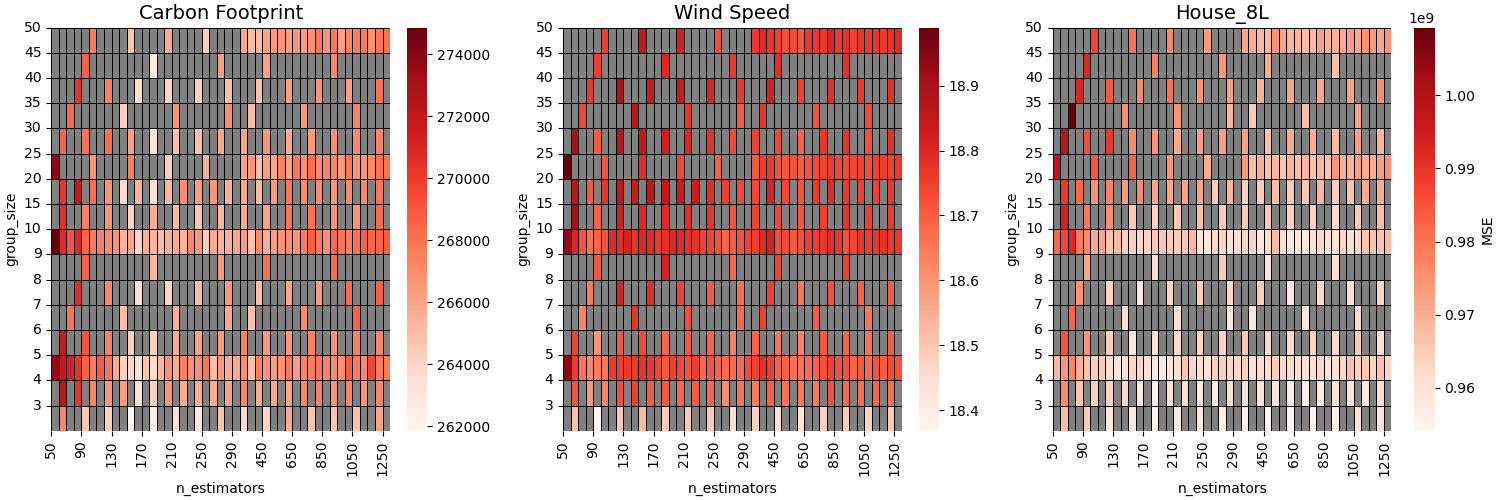
\includegraphics[width=1\textwidth]{figures/marco-metodologico/heatmaps/heatmap_iqr.png}
\caption{Relación entre hiperparámetros y MSE para el modelo \texttt{IQRRandomForestRegressor}}
\end{figure}
\label{figure4}

\begin{figure}[h]
\centering
    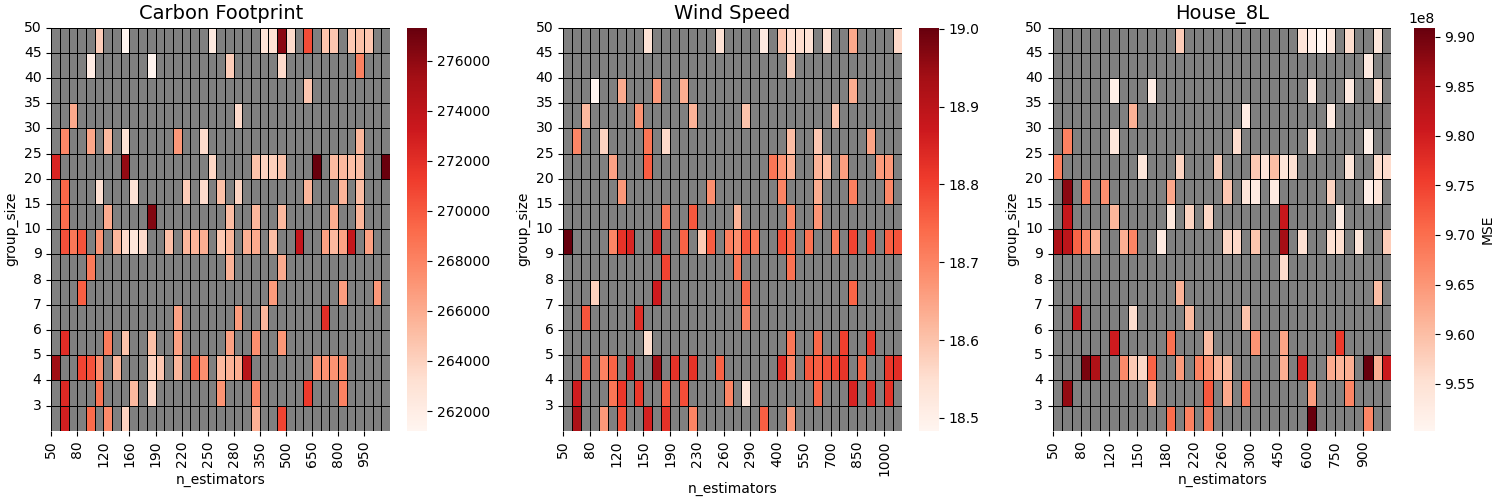
\includegraphics[width=1\textwidth]{figures/marco-metodologico/heatmaps/heatmap_pt_2.png}
\caption{Relación entre hiperparámetros \texttt{group\_size} y \texttt{n\_estimators} y MSE para el modelo \texttt{PercentileTrimmingRandomForestRegressor} con \texttt{percentile=2}}
\end{figure}
\label{figure5}

\begin{figure}[h]
\centering
    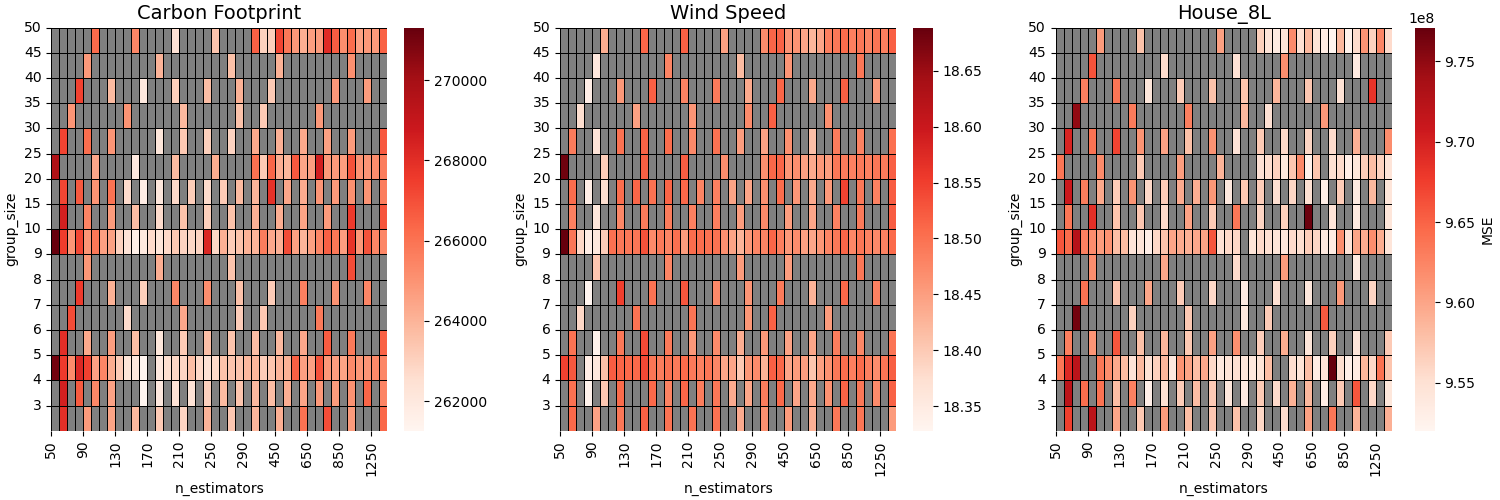
\includegraphics[width=1\textwidth]{figures/marco-metodologico/heatmaps/heatmap_oob.png}
\caption{Relación entre hiperparámetros \texttt{group\_size} y \texttt{n\_estimators} y MSE para el modelo \texttt{OOBRandomForestRegressor}}
\end{figure}
\label{figure6}

\begin{figure}[h]
\centering
    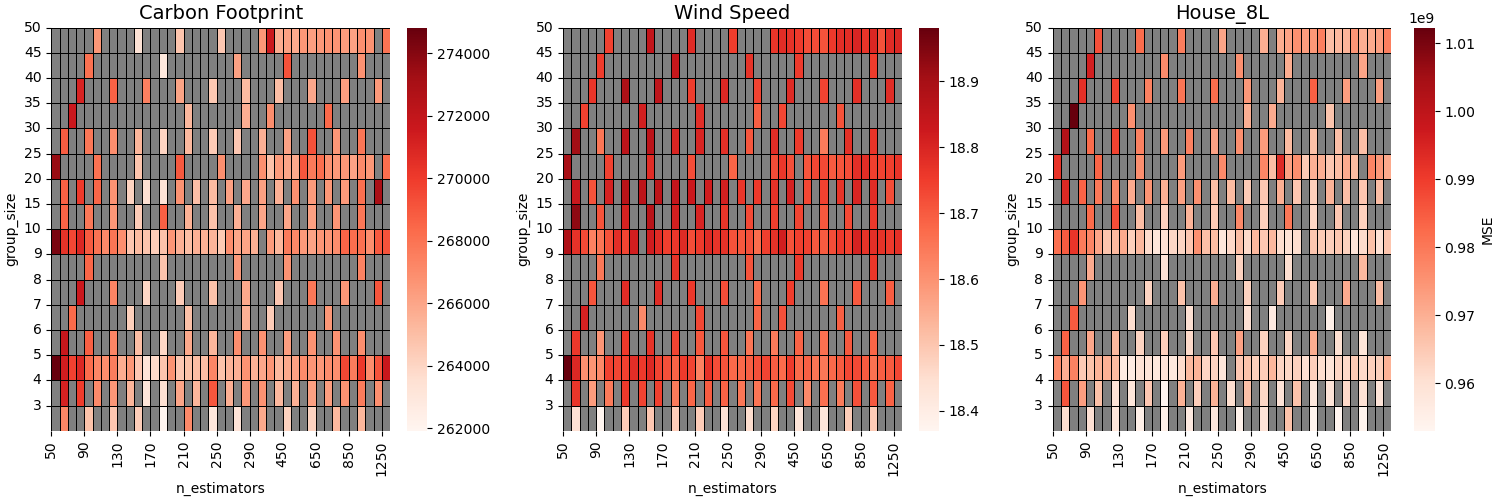
\includegraphics[width=1\textwidth]{figures/marco-metodologico/heatmaps/heatmap_oob_plus_iqr.png}
\caption{Relación entre hiperparámetros \texttt{group\_size} y \texttt{n\_estimators} y MSE para el modelo \texttt{OOBPlusIQRRandomForestRegressor}}
\end{figure}
\label{figure7}

\begin{figure}[h]
\centering
    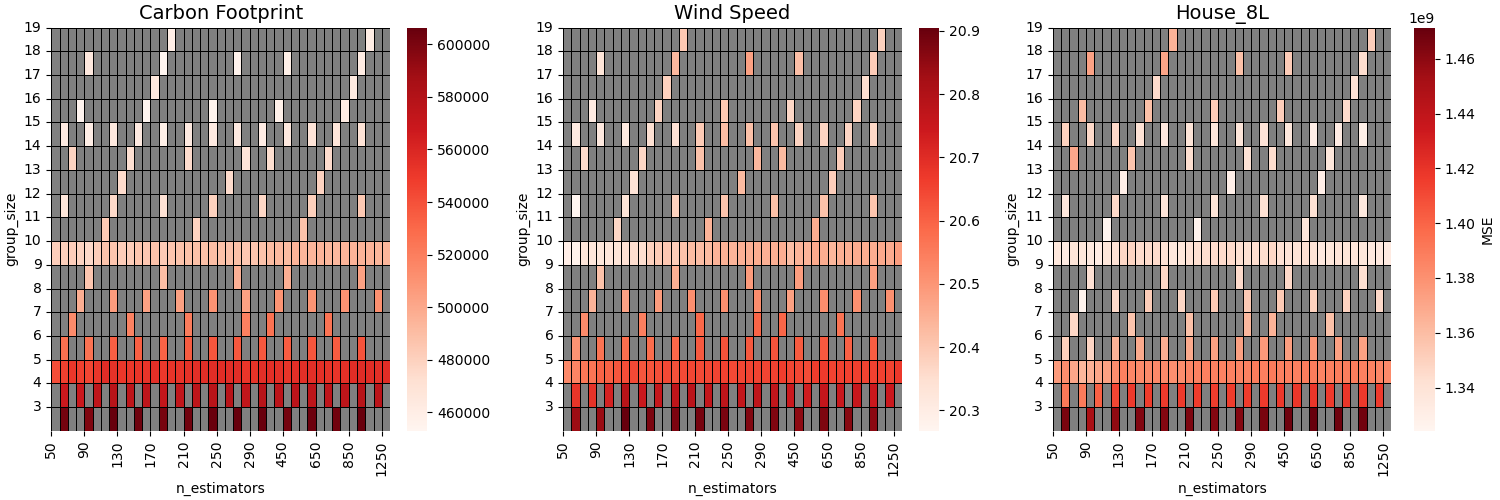
\includegraphics[width=1\textwidth]{figures/marco-metodologico/heatmaps/heatmap_fsc.png}
\caption{Relación entre hiperparámetros \texttt{group\_size} y \texttt{n\_estimators} y MSE para el modelo \texttt{FirstSplitCombinerRandomForestRegressor}}
\end{figure}
\label{figure8}

\begin{figure}[h]
\centering
    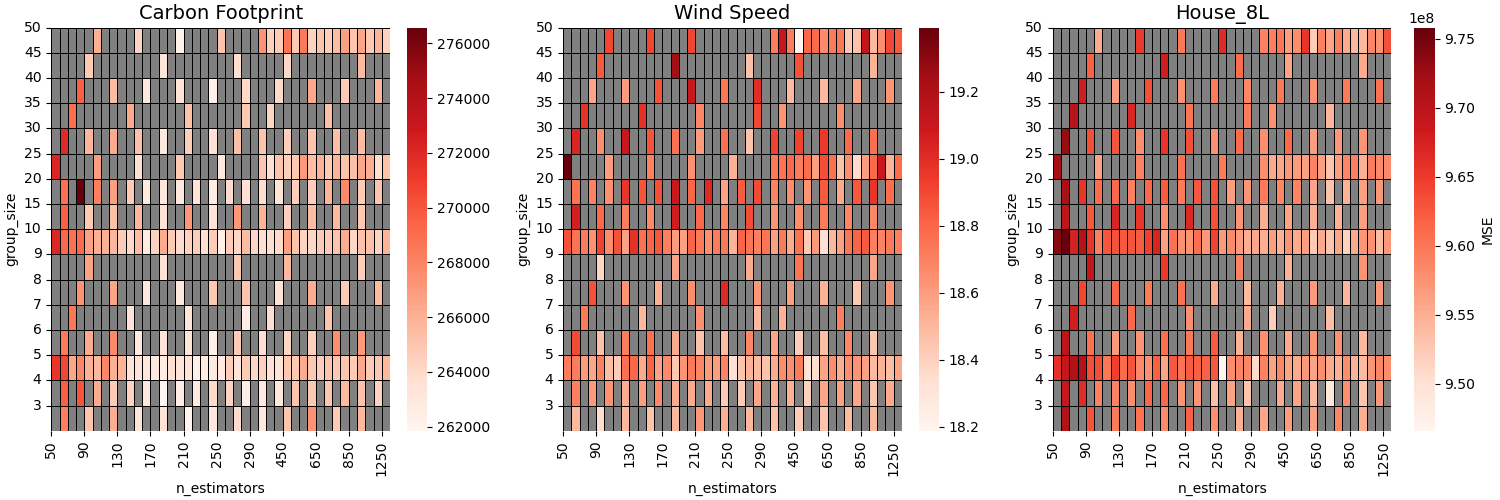
\includegraphics[width=1\textwidth]{figures/marco-metodologico/heatmaps/heatmap_sk.png}
\caption{Relación entre hiperparámetros \texttt{group\_size} y \texttt{n\_estimators} y MSE para el modelo \texttt{SharedKnowledgeRandomForestRegressor}}
\end{figure}
\label{figure9}

\FloatBarrier

\begin{figure}[h]
\centering
    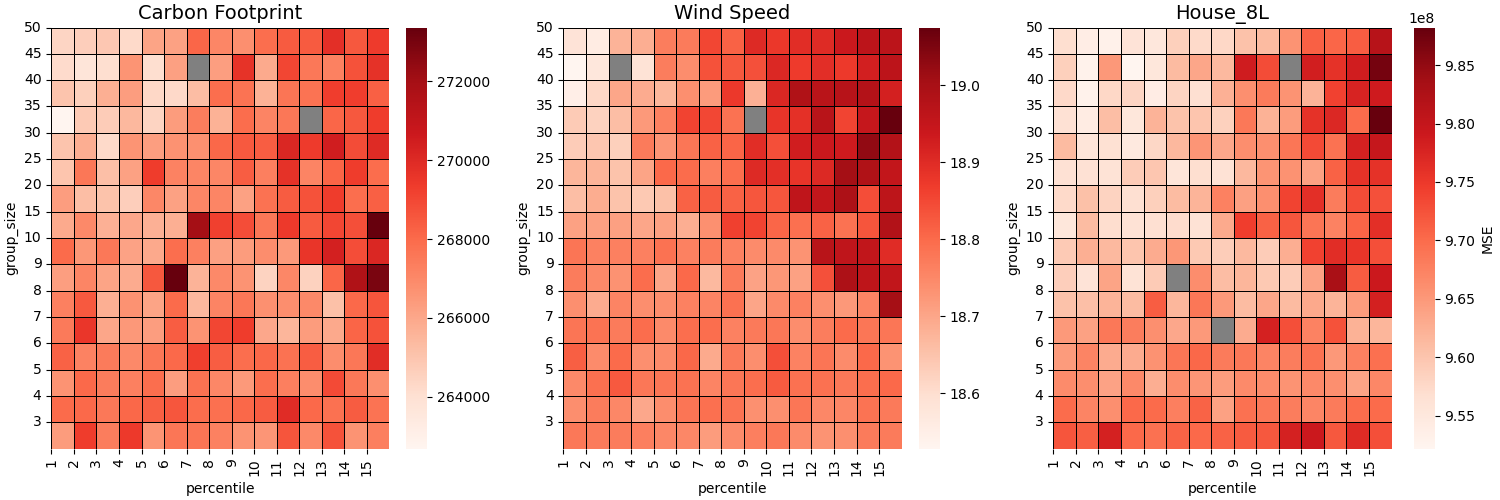
\includegraphics[width=1\textwidth]{figures/marco-metodologico/heatmaps/heatmap_percentile_vs_group_size.png}
\caption{Relación entre hiperparámetros \texttt{group\_size} y \texttt{percentile} y MSE para el modelo \texttt{PercentileTrimmingRandomForestRegressor}}
\end{figure}
\label{figure10}



Un patrón en común entre todos los modelos y los datasets es que, en general, las configuraciones de hiperparámetros que mejor resultados obtienen son aquellas que tienen un número moderado de árboles total (entre $100$ y $300$) y grupos de tamaños relativamente chicos. Esto de puede notar en los mapas de calor observando el tono más claro de las esquinas inferiores izquierdas. Sin embargo, hay dos modelos los cuáles tienen particularidades.

Para el caso particular del \texttt{FirstSplitCombinerRandomForestRegressor}, se nota claramente con los mapas de calor que este modelo requiere tamaños de grupos mayores, dado que la parte inferior de los mismos se los ve más oscuros indicando mayor MSE, es decir peor rendimiento. Esto tiene muchos sentido dado la naturaleza misma del modelo. Al depender la capacidad predictiva del modelo en los árboles combinados por grupo y considerando que se toma el primer corte de cada árbol del grupo, cuanto mayor sea el tamaño del grupo mayor será la profundidad de los árboles combinados, permitiendo capturar más información de los datos.

Por su parte, en cuanto al modelo \texttt{PercentileTrimmingRandomForestRegressor}, en la \hyperref[figure10]{Figura 10} se observa la relación entre los hiperparámetros \texttt{group\_size} y \texttt{percentile}, donde se puede observar que las mejores combinaciones entre estos dos ocurre con un tamaño de grupo grande y porcentaje de exclusión en los extremos bajos. Esto tiene sentido dado que, a diferencia del modelo que utiliza IQR, este siempre elimina de ambos extremos por lo que para no perder tanta información en el promedio grupal, se necesitan más árboles por grupo. A su vez, percentiles mayores a 5 ya significa la pérdida de mucha información. Por esto motivo se ve que la \hyperref[figure5]{Figura 5} se filtran aquellas configuraciones dónde se uso percentil igual a dos, para a partir de ahí notar la cantidad de árboles totales más óptima.

Para los demás hiperparámetros específicos de cada modelo como \texttt{initial\_max\_depth} o \texttt{max\_features}, se definieron una vez establecidos los principales a partir de la  comparación simple del valor de MSE de las distintas configuraciones. El hiperparámetro \texttt{max\_features} fue sólo tenido en cuenta en \texttt{FirstSplitCombinerRandomForestRegressor} dado que era dónde se veía más neceserario ajustarlo. Para el resto de modelos se dejó este hiperparámetro como se ecuentra en el default de la librería de código abierto, que es en $1$, es decir que se usan todas las features en todos los árboles. 

El caso del hiperparámetro \texttt{max\_depth} fue un caso particular. Al ser un parámetro de naturaleza regularizador ya que controla que los árboles no sobre-ajusten a los datos, el mismo depende mucho del problema a evaluar, es decir del dataset. Por eso motivo, se decidió no definir un valor predeterminado para el mismo, sino que esté optimizado según cada modelo y dataset.

En base al análisis global de los hiperparámetros y su interrelación fue que quedaron conformados los valores predeterminados para cada modelo y dataset. Si bien el procedimiento llevado a cabo no asegura encontrar la configuración óptima \textit{global}, permite identificar parámetros con un desempeño eficiente dentro de un tiempo razonable.

\section{Comparación de modelos}

Teniendo los modelos con sus hiperparámetros definidos\footnote{Valores por modelo y dataset en \hyperref[appendix7]{Apéndice 7}.}, utilizamos los datos reservados para testing para evaluar si alguno presenta mejoras significativas en desempeño en comparación con el algoritmo original \textbf{\texttt{RandomForestRegressor}}. Para esto debemos llevar a cabo un test no paramétrico llamado Kruskal-Wallis, el cual se basa en las siguientes hipótesis:

\begin{itemize}
    \item \textit{Hipótesis nula ($H_0$)}: No hay diferencias significativas en el MSE entre los modelos evaluados, incluido el \texttt{RandomForestRegressor}.

    \item \textit{Hipótesis alternativa ($H_1$)}: Al menos uno de los modelos tiene un MSE significativamente diferente al de \texttt{RandomForestRegressor}.
\end{itemize}

El siguiente procedimiento se llevó a cabo para los tres datasets principales, y luego los otros tres adicionales. En primer lugar, realizamos una validación cruzada de 10-folds, asegurándonos de que todos los modelos utilicen exactamente los mismos conjuntos de entrenamiento y validación mediante una semilla. Esto genera, para cada modelo, un conjunto de 10 valores de MSE, y se agrupan en una lista específica para cada modelo. 

Con las listas generadas, usamos el test de \textit{\textbf{Kruskal-Wallis}} (KW) para comparar simultáneamente los MSEs de todos los modelos. Este análisis permite identificar si existen diferencias significativas entre los modelos; un valor alto en el test KW, y su p-valor asociado, indica dichas diferencias. 

El test Kruskal-Wallis permite identificar si existen diferencias significativas entre los modelos evaluados, pero no proporciona información sobre cuáles modelos específicos presentan dichas diferencias. Debido a esto, en caso en que se rechace la hipótesis nula ($H_0$) y obtenemos un p-valor menor a $0.05$, realizamos un análisis \textit{post-hoc} utilizando el test de \textit{Dunn} para determinar qué pares de modelos son significativamente diferentes. De este test se obtendrá una matriz, presentada en \hyperref[ch::capitulo7]{\textit{Resultados}}, que compara cada modelo con los demás para identificar dónde están las diferencias.

% called by main.tex
%
\chapter{Resultados}
\label{ch::capitulo7}

En este capítulo se presentan los datos resultantes de la investigación con el fin de observar el rendimiento de los diferentes modelos implementados y su comparación entre sí. 

En la \hyperref[figure11]{Figura 11}, se pueden observar para cada conjunto de datos evaluados, la mediana del MSE entre las distintas particiones de la evaluación \textit{Cross-Validation} para los modelos:

\begin{itemize}
    \item \texttt{RandomForestRegressor} (RF),
    \item \texttt{SharedKnowledgeRandomForestRegressor} (SK),
    \item \texttt{OOBRandomForestRegressor} (OOB),
    \item \texttt{IQRRandomForestRegressor} (IQR),
    \item \texttt{OOBPlusIQRRandomForestRegressor} (OOB+IQR),
    \item \texttt{PercentileTrimmingRandomForestRegressor} (PT) y
    \item \texttt{FirstSplitCombinerRandomForestRegressor} (FSC).
\end{itemize}

Con mayor detalle se presentan las mediciones para cada fold, dataset y modelo en el \hyperref[appendix8]{Apéndice 8}.

\begin{figure}[h]
\centering
    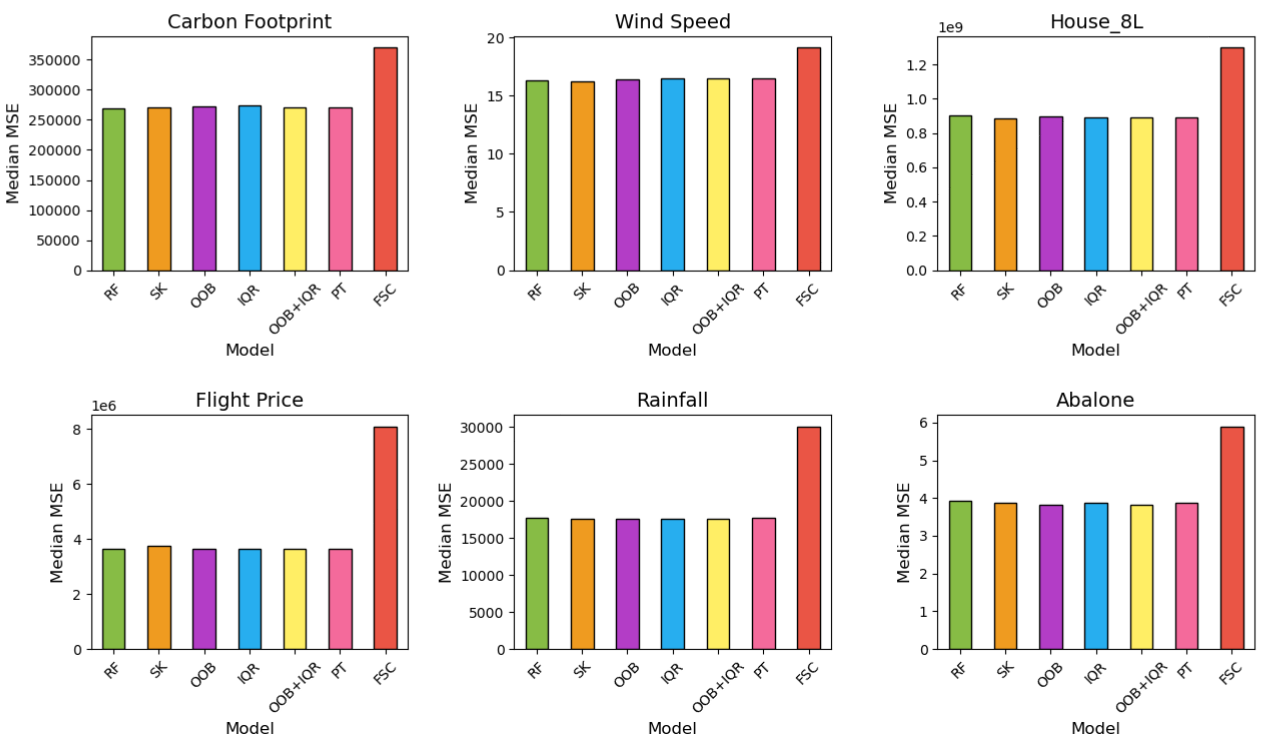
\includegraphics[width=1\textwidth]{figures/results/comparison_grid.png}
\caption{Mediana del MSE por modelo en cada dataset}
\end{figure}
\label{figure11}

\FloatBarrier

Por su parte, en la \hyperref[tab1]{Tabla 1} se presentan los resultados del test de hipótesis no paramétrico evaluado para comparar los modelos entre sí para cada uno de los conjuntos de datos seleccionados.

\begin{table}[h!]
\centering
\begin{tabular}{lcc}
\toprule
\textbf{Dataset} & \textbf{H-statistic} & \textbf{p-valor} \\
\midrule
Carbon Footprint & 20.4  & 0.002 \\
House 8L         & 13.5  & 0.035 \\
Wind Speed       & 7.86  & 0.25 \\
Rainfall         & 25.65 & 0.0003 \\
Flight Price     & 14.09 & 0.029 \\
Abalone          & 20.76 & 0.0020 \\
\bottomrule
\end{tabular}
\caption{Resultados del test de Kruskal-Wallis.}
\label{tab1}
\end{table}

\FloatBarrier

A su vez, para aquellos conjunto de datos en los cuáles se observó alguna diferencia significativa entre modelos, se muestran en las Tablas \hyperref[tab2]{2}, \hyperref[tab3]{3}, \hyperref[tab4]{4}, \hyperref[tab5]{5} y \hyperref[tab6]{6} los resultados del análisis post-hoc utilizando el test de Dunn.

\section*{}

\begin{longtable}{lccccccc}
\toprule
   & IQR     & PT     & OOB     & OOB+IQR     & FSC      & SK     & RF     \\
\midrule
IQR  & 1.0   & 1.0   & 1.0   & 1.0   & 0.015  & 1.0   & 1.0   \\
PT  & 1.0   & 1.0   & 1.0   & 1.0   & 0.014  & 1.0   & 1.0   \\
OOB  & 1.0   & 1.0   & 1.0   & 1.0   & 0.010  & 1.0   & 1.0   \\
OOB+IQR  & 1.0   & 1.0   & 1.0   & 1.0   & 0.012  & 1.0   & 1.0   \\
FSC  & 0.015 & 0.014 & 0.010 & 0.012 & 1.0    & 0.009 & 0.012 \\
SK  & 1.0   & 1.0   & 1.0   & 1.0   & 0.009  & 1.0   & 1.0   \\
RF  & 1.0   & 1.0   & 1.0   & 1.0   & 0.012  & 1.0   & 1.0   \\
\bottomrule
\caption{Carbon Footprint}
\end{longtable}
\label{tab2}

\begin{longtable}{lccccccc}
\toprule
   & IQR     & PT     & OOB     & OOB+IQR     & FSC      & SK     & RF     \\
\midrule
IQR  & 1.0   & 1.0   & 1.0   & 1.0   & 0.165  & 1.0   & 1.0    \\
PT  & 1.0   & 1.0   & 1.0   & 1.0   & 0.114  & 1.0   & 1.0    \\
OOB  & 1.0   & 1.0   & 1.0   & 1.0   & 0.100  & 1.0   & 1.0    \\
OOB+IQR  & 1.0   & 1.0   & 1.0   & 1.0   & 0.081  & 1.0   & 1.0    \\
FSC  & 0.165 & 0.114 & 0.100 & 0.081 & 1.0    & 0.068 & 0.159  \\
SK  & 1.0   & 1.0   & 1.0   & 1.0   & 0.068  & 1.0   & 1.0    \\
RF  & 1.0   & 1.0   & 1.0   & 1.0   & 0.159  & 1.0   & 1.0    \\
\bottomrule
\caption{House\_8L}
\end{longtable}
\label{tab3}

\begin{longtable}{lccccccc}
\toprule
   & IQR     & PT     & OOB     & OOB+IQR     & FSC      & SK     & RF     \\
\midrule
IQR  & 1.0   & 1.0   & 1.0   & 1.0   & 0.001  & 1.0   & 1.0    \\
PT  & 1.0   & 1.0   & 1.0   & 1.0   & 0.009  & 1.0   & 1.0    \\
OOB  & 1.0   & 1.0   & 1.0   & 1.0   & 0.002  & 1.0   & 1.0    \\
OOB+IQR  & 1.0   & 1.0   & 1.0   & 1.0   & 0.002  & 1.0   & 1.0    \\
FSC  & 0.001 & 0.009 & 0.002 & 0.002 & 1.0    & 0.001 & 0.003  \\
SK  & 1.0   & 1.0   & 1.0   & 1.0   & 0.001  & 1.0   & 1.0    \\
RF  & 1.0   & 1.0   & 1.0   & 1.0   & 0.003  & 1.0   & 1.0    \\
\bottomrule
\caption{Rainfall}
\end{longtable}
\label{tab4}

\begin{longtable}{lccccccc}
\toprule
   & IQR     & PT     & OOB     & OOB+IQR     & FSC      & SK     & RF     \\
\midrule
IQR  & 1.0   & 1.0   & 1.0   & 1.0   & 0.078  & 1.0   & 1.0    \\
PT  & 1.0   & 1.0   & 1.0   & 1.0   & 0.107  & 1.0   & 1.0    \\
OOB  & 1.0   & 1.0   & 1.0   & 1.0   & 0.070  & 1.0   & 1.0    \\
OOB+IQR  & 1.0   & 1.0   & 1.0   & 1.0   & 0.070  & 1.0   & 1.0    \\
FSC  & 0.078 & 0.107 & 0.070 & 0.070 & 1.0    & 0.213 & 0.070  \\
SK  & 1.0   & 1.0   & 1.0   & 1.0   & 0.213  & 1.0   & 1.0    \\
RF  & 1.0   & 1.0   & 1.0   & 1.0   & 0.070  & 1.0   & 1.0    \\
\bottomrule
\caption{Flight Price}
\end{longtable}
\label{tab5}

\begin{longtable}{lccccccc}
\toprule
   & IQR     & PT     & OOB     & OOB+IQR     & FSC      & SK     & RF     \\
\midrule
IQR  & 1.0   & 1.0   & 1.0   & 1.0   & 0.010  & 1.0   & 1.0    \\
PT  & 1.0   & 1.0   & 1.0   & 1.0   & 0.013  & 1.0   & 1.0    \\
OOB  & 1.0   & 1.0   & 1.0   & 1.0   & 0.006  & 1.0   & 1.0    \\
OOB+IQR  & 1.0   & 1.0   & 1.0   & 1.0   & 0.006  & 1.0   & 1.0    \\
FSC  & 0.010 & 0.013 & 0.006 & 0.006 & 1.0    & 0.016 & 0.024  \\
SK  & 1.0   & 1.0   & 1.0   & 1.0   & 0.016  & 1.0   & 1.0    \\
RF  & 1.0   & 1.0   & 1.0   & 1.0   & 0.024  & 1.0   & 1.0    \\
\bottomrule
\caption{Abalone}
\end{longtable}
\label{tab6}

Dada la diferencia particular del modelo \texttt{FirstSplitCombinerRandomForestRegressor}, de la cuál se desarrolla en \textit{\hyperref[ch::capitulo8]{Discusión}}, se re-evaluó el test de hipótesis quitando este modelo. Estos resultados se ven en la \hyperref[tab7]{Tabla 7}.

\begin{table}[h!]
\centering
\begin{tabular}{lcc}
\toprule
\textbf{Dataset} & \textbf{H-statistic} & \textbf{p-valor} \\
\midrule
Carbon Footprint & 0.04  & 0.99 \\
House 8L         & 0.18  & 0.99 \\
Wind Speed       & 0.13  & 0.99 \\
Rainfall         & 0.40 & 0.99 \\
Flight Price     & 0.25 & 0.99 \\
Abalone          & 0.30 & 0.99 \\
\bottomrule
\end{tabular}
\caption{Resultados del test de Kruskal-Wallis sin el modelo FSC.}
\label{tab7}
\end{table}

% called by main.tex
%
\chapter{Discusión}
\label{ch::capitulo8}

En esta sección, nos proponemos interpretar los resultados obtenidos y expuestos anteriormente. Al mismo tiempo, se buscará analizar los hallazgos y discutir las posibles causas de lo observado en concordancia con el trabajo de experimentación llevado a cabo.

En primer lugar, el resultado más relevante es el rendimiento observado de las variantes propuestas de RF que incorporan la etapa intermedia de debate en comparación al algoritmo clásico. Como se puede ver una vez ejecutado el test de hipótesis no paramétrico Kruskal-Wallis sobre los diferentes modelos, existen diferencias significativas entre los mismos para cinco de los seis conjuntos de entrenamiento evaluados. Esto se deriva de que el p-valor obtenido fue menor a $0.05$, con excepción del dataset \textit{Wind} (ver \hyperref[tab1]{Tabla 1}).

Sin embargo, con el análisis post-hoc utilizando el test de Dunn, se puede observar entre las comparaciones modelo a modelo, que el único modelo que presenta diferencias significativas con el resto es \texttt{FirstSplitCombinerRandomForestRegressor}. Esto mismo se puede notar dado que la matriz resultante del análisis de Dunn, muestra unos para todas las columnas y filas, a excepción de la fila y columna correspondiente al modelo de combinación árboles de primeros cortes. A su vez, se puede verificar lo mismo observando el orden para los distintos datasets entre los modelos para cada fold del cross-validation llevado a cabo. Para muchos de los folds, el modelo en cuestión se encuentra al final de la tabla indicando que su performance en comparación de los otros modelos fue inferior. También se puede constatar esto mismo en la \hyperref[figure11]{Figura 11}, dónde se ve la mediana para cada modelo entre los distintos folds, donde el modelo de combinación de árboles tiene una mediana efectivamente superior de MSE que el resto de los modelos y, a su vez, entre los otros modelos no se notan prácticamente diferencias visualmente.

Con esa información, entonces, podemos confirmar que el modelo de combinación de árboles de primeros cortes tiene efectivamente un rendimiento inferior en comparación tanto del modelo original como de las otras alternativas propuestas. Por otro lado, al quitar al modelo de combinación del análisis y evaluar nuevamente con el test no paramétrico vemos que claramente los p-valores son mucho más grandes que $0.05$ por lo que no hay evidencia suficiente para rechazar la hipótesis nula del test. Esto demuestra que las variaciones que incluyen la simulación del debate entre árboles exploradas en este trabajo no mostraron mejoras significativas con respecto al algoritmo de RF clásico, contrario a la hipótesis planteada.

Si bien no pudo ser confirmada la hipótesis de que un algoritmo de ensamble como RF mejore su rendimiento con mecanismos de agregación entre predicciones diferentes, tampoco se puede descartar por completo la hipótesis. A lo largo de este trabajo, si bien se exploraron numerosas alternativas de simulación de etapa intermedia de deliberación, podrían haber mecanismos no explorados que imiten de manera más eficiente lo observado con personas en el experimento de psicología experimental llevado a cabo por Navajas.

Además, observando con detenimiento las tablas con el orden de resultados, se puede notar que para algunos conjuntos de instancias de validación (folds), algunas de las variantes propuestas en esta investigación superaron al algoritmo original. Esto puede motivar a pensar que futuros ajustes y refinamientos ya sea de las implementaciones u optimización de hiperparámetros no explorados permitan una mejora significativa.

Enfocándonos ahora en los motivos de estos resultados, existen diversas interpretaciones e ideas que se pueden plantear. Con respecto a por qué el modelo de combinación de árboles de primeros cortes (FSC) tuvo un rendimiento por lejos inferior que el resto, consideramos que el principal motivo se encuentra en la naturaleza de la combinación misma de árboles. Recordando esta implementación, para combinar los árboles se toma únicamente el primer corte o división de los mismos. Observando algunas instancias de evaluación se puede notar que, si bien controlado por el hiperparámetro \texttt{max\_features} no todos los árboles tuvieron a disposición las mismas features, cada árbol que tenga la característica óptima de corte la utilizará para su primer división. De esta forma, para cada grupo de árboles, puede suceder que varios árboles tengan como feature de primer corte a la misma variable con pequeñas variaciones en el valor del umbral de división. Eso provocará que a lo largo de los niveles del árbol combinado se repita la misma variable de corte haciendo que el árbol tenga sucesivos cortes que no aporten información y sean redundantes. Es así como, muy probablemente cada árbol combinado perdió información valiosa de los árboles iniciales provocando que el modelo pierda capacidad predictiva.

Por otro lado, el hecho de que para el dataset \textit{Wind}, no haya diferencias significativas con \texttt{FirstSplitCombinerRandomForestRegressor} podría ser causa de particularidades específicas del conjunto de datos en cuestión. En este caso, es un conjunto de datos con diez variables numéricas. Una posible explicación es que al ser relativamente no muchas features, el hiperparámetro \texttt{max\_features} forzó a que los árboles usen como primer corte diversas features, provocando que el problema de redundancia tenga un impacto mucho menor que para los otros conjuntos de entrenamiento. Esto indicaría que el modelo de combinación de árboles de primeros cortes, en algunas circunstancias, no tendría una performance significativamente inferior al resto. Sin embargo, dado que esto sólo ocurre en uno de los seis datasets, no modifica sustancialmente las conclusiones descritas anteriormente.

Otra observación a notar de los resultados es la relación entre la performance de los modelos y el cumplimiento de la distribución de Navajas. En los conjuntos de entrenamiento cuyas predicciones no siguen la distribución log-normal, no se evidencia una diferencia significativa en la performance en comparación con RF. Esto podría indicar que para las alternativas exploradas, la distribución no es un factor determinante para la performance de los modelos. Sin embargo, hay un pequeño detalle que se puede notar observando con detenimiento la tabla de ranking de \textit{cross-validation} (\hyperref[appendix8]{Apéndice 8}). Para aquellos conjuntos de datos con los que las predicciones de los árboles no siguen una distribución log-normal, se nota que los modelos \texttt{OOBRandomForestRegressor} y \texttt{OOBPlusIQRRandomForestRegressor} presentan resultados idénticos. Esto muy posiblemente se deba a que entre las predicciones de los árboles en cada grupo no hay \textit{outliers} claros por lo que el mecanismo de exclusión en \texttt{OOBPlusIQRRandomForestRegressor} no tiene ningún impacto. Además, estos modelos tienen como hiperparámetros \texttt{n\_estimators} y \texttt{group\_size} los mismos valores. Para verificar esta hipótesis, realizamos una ejecución de los modelos en cuestión sumado a \texttt{IQRRandomForestRegressor} y RF original. Se puede notar en la tabla del \hyperref[appendix9]{Apéndice 9} que, ante los mismos valores de \texttt{n\_estimators} y \texttt{max\_depth}, entre \texttt{OOBRandomForestRegressor} y \texttt{OOBPlusIQRRandomForestRegressor} por un lado y entre \texttt{IQRRandomForestRegressor} y RF original, los MSE que arrojan coinciden. Esto sustenta la teoría que la exclusión por el método de IQR no sirve para datasets que no cumplen las condiciones descriptas previamente.

Finalmente, en cuanto a las razones por la que no se notaron diferencias significativas entre las demás variantes y RF original, no parecen haber motivos o causas que se puedan identificar de manera sencilla. Un posible motivo, el cual consideramos bastante probable, es que si bien nuestras alternativas son diversas conceptualmente entre si y con el algoritmo original, todas tienen un fuerte foco en la etapa de agregación de información entre los árboles individuales y no alteran sustancialmente la fase de entrenamiento de los mismos. 

Otros modelos de ensamble que han tomado ideas similares a Random Forest y han logrado superarlo, como puede ser \textit{XGBoost}, trabajan de lleno con la construcción inicial de los árboles. Este enfoque puede tener un mayor peso sobre la capacidad predictiva del modelo que la manera de ensamblar en sí, siempre y cuando esta sea razonable. Los malos resultados obtenidos en FSC podrían acercarnos a esta posible explicación, dado que su manera de combinar los árboles es la mas alejada de la del algoritmo original, mientras que los otros algoritmos de alguna forma u otra terminan realizando también un promedio.

% called by main.tex
%
\chapter{Conclusiones \& Recomendaciones}
\label{ch::capitulo9}

Haciendo un balance del trabajo, podemos afirmar que logramos cumplir con los objetivos que nos planteamos en un comienzo, los cuales se encuentran detallados en la sección \hyperref[ch::capitulo3]{\textit{Objetivos del proyecto}}. 

En primer lugar, logramos comprender en detalle tanto el algoritmo de Random Forest como su implementación concreta en la librería \textit{Scikit-learn}, así como los conceptos y principios fundamentales que lo sustentan. Por otro lado, obtuvimos datos de entrenamiento con distribuciones similares a las observadas en los resultados de \cite{navajasAggregatedKnowledge} y le realizamos la ingeniería de datos necesaria para el correcto funcionamiento de nuestras propuestas y el algoritmo original de Random Forest. 

A partir de allí, ideamos propuestas de simulación de debate para las ideas que habíamos planteado en un inicio, como la exclusión de extremos en grupos con los modelos \texttt{IQRRandomForestRegressor} y \texttt{PercentileTrimmingRandomForestRegressor}, el uso del promedio como en el algoritmo original, pero editado para ser ponderado por una confianza, con el modelo \texttt{OOBRandomForestRegressor}, y la combinación de árboles, mediante la idea de unir los primeros cortes, implementada en \texttt{FirstSplitCombinerRandomForestRegressor}. 

A su vez,  a lo largo del proyecto y mientras implementamos estas propuestas, fueron surgiendo nuevas, como la combinación entre el promedio ponderado por confianza y la exclusión de extremos, lo cual implementamos en nuestro modelo \texttt{OOBPlusIQRRandomForestRegressor} y una nueva propuesta de conocimiento compartido, utilizada en el último modelo explorado \texttt{SharedKnowledgeRandomForestRegressor}.

Con todos estos modelos implementados, optimizamos cada uno de ellos realizando una gran barrida de hiperparámetros en rangos razonables, y finalmente, con todos los modelos implementados y optimizados, realizamos tests estadísticos y visualizaciones para compararlos entre sí y con el modelo original.

Si bien tras estos tests, encontramos que nuestras alternativas que simulan la etapa intermedia de “debate” no resultaron en modelos significativamente superiores al Random Forest original, sí pudimos encontrar que algunas de ellas obtienen resultados similares en promedio, siendo en algunos casos levemente mejores y en otros casos levemente inferiores. Esto, nos motiva a plantear posibles iteraciones para el futuro, como podría ser realizar una contribución a la librería open-source \textit{Scikit-learn} para que estas modificaciones queden como modelos alternativos a considerar para diferentes aplicaciones o instancias en las cuáles supere al state-of-art. Por su parte, al igual que discutido anteriormente, se podría probar qué sucede si se continúa con la optimización de las alternativas, utilizando los diversos hiperparámetros que posee el algoritmo original y que por una cuestión de tiempo, quedaron fuera del alcance de nuestro proyecto para evaluar. Adicionalmente, así como surgió el modelo de \texttt{OOBPlusIQRRandomForestRegressor} a partir de sumar ideas de simulación exploradas en otros modelos, de igual manera se podría seguir explorando otras combinaciones. Por ejemplo, se le podría sumar al modelo de conocimiento compartido, etapas posteriores a la construcción de árboles extendidos como la exclusión de extremos o la ponderación por confianza. 

También notamos que, si bien nuestras propuestas para el debate incluyen muchas formas distintas de combinar el conocimiento de los árboles, no tienen en cuenta el replanteo del problema desde cero que se puede dar durante la deliberación. Este aspecto es algo que podría ser fundamental para la mejora en las predicciones, dado que los seres humanos al debatir tienen la capacidad de barajar y dar de nuevo con la pregunta en cuestión e ir consensuando la respuesta, sin necesidad de combinar las respuestas originales que cada uno había pensado. Simulaciones nuevas de debate entre árboles que utilicen estos conceptos podrían ser interesantes de explorar y abren la puerta a nuevas líneas de investigación a la vez que surgen nuevos estudios del comportamiento humano que comprendan mejor el proceso de deliberación entre personas.

Por otro lado, podría ser también interesante explorar la simulación de otras consideraciones en el debate entre personas, en particular, el rol de la \textit{presión social} que provocan las opiniones de los demás a la hora de tomar una decisión. En nuestro caso, este aspecto podría ser tenido en cuenta en nuestro último modelo de conocimiento compartido simulando el impacto que tiene las predicciones de los otros árboles, análogamente a cómo afectan las opiniones de otras personas. Quizás, con las modificaciones necesarias, se podría, partiendo de la idea del modelo \texttt{SharedKnowledgeRandomForestRegressor}, simular el efecto de \textit{presión social}.

Más allá de las definiciones formales de la \textit{presión social}, se la puede pensar como un mayor peso de la información de los demás por sobre otra. Esto se podría efectivamente simular dándole un mayor peso a las features otorgadas por otros árboles del grupo, por ejemplo con una mayor probabilidad de ser seleccionadas para el corte, o dándoles una ventaja a la hora de compararse frente a otras alternativas de corte en cada nivel durante entrenamiento. Sería probable hacer que esta presión pueda ser ajustada mediante un hipotético nuevo hiperparámetro llamado “pressure”.

Finalmente, Random Forest es solo uno de los varios modelos de ensamble que existen. Nuevos enfoques de investigación podrían ser evaluar simulaciones con propuestas similares a las de este proyecto en otros modelos de ensamble, o si se encuentra algún mecanismo de agregación más sofisticado y eficiente que modele el debate.


% \cleardoublepage

% --------------------------
% Back matter
% --------------------------
\backmatter

\printbibliography[title=Referencias, heading=bibintoc]

\appendix
% called by main.tex
%
\chapter{Apéndices}
\label{ch::capitulo10}

\section*{1. Figuras distribución datos originales}
 \label{appendix1}

\begin{figure}[h]
\centering
    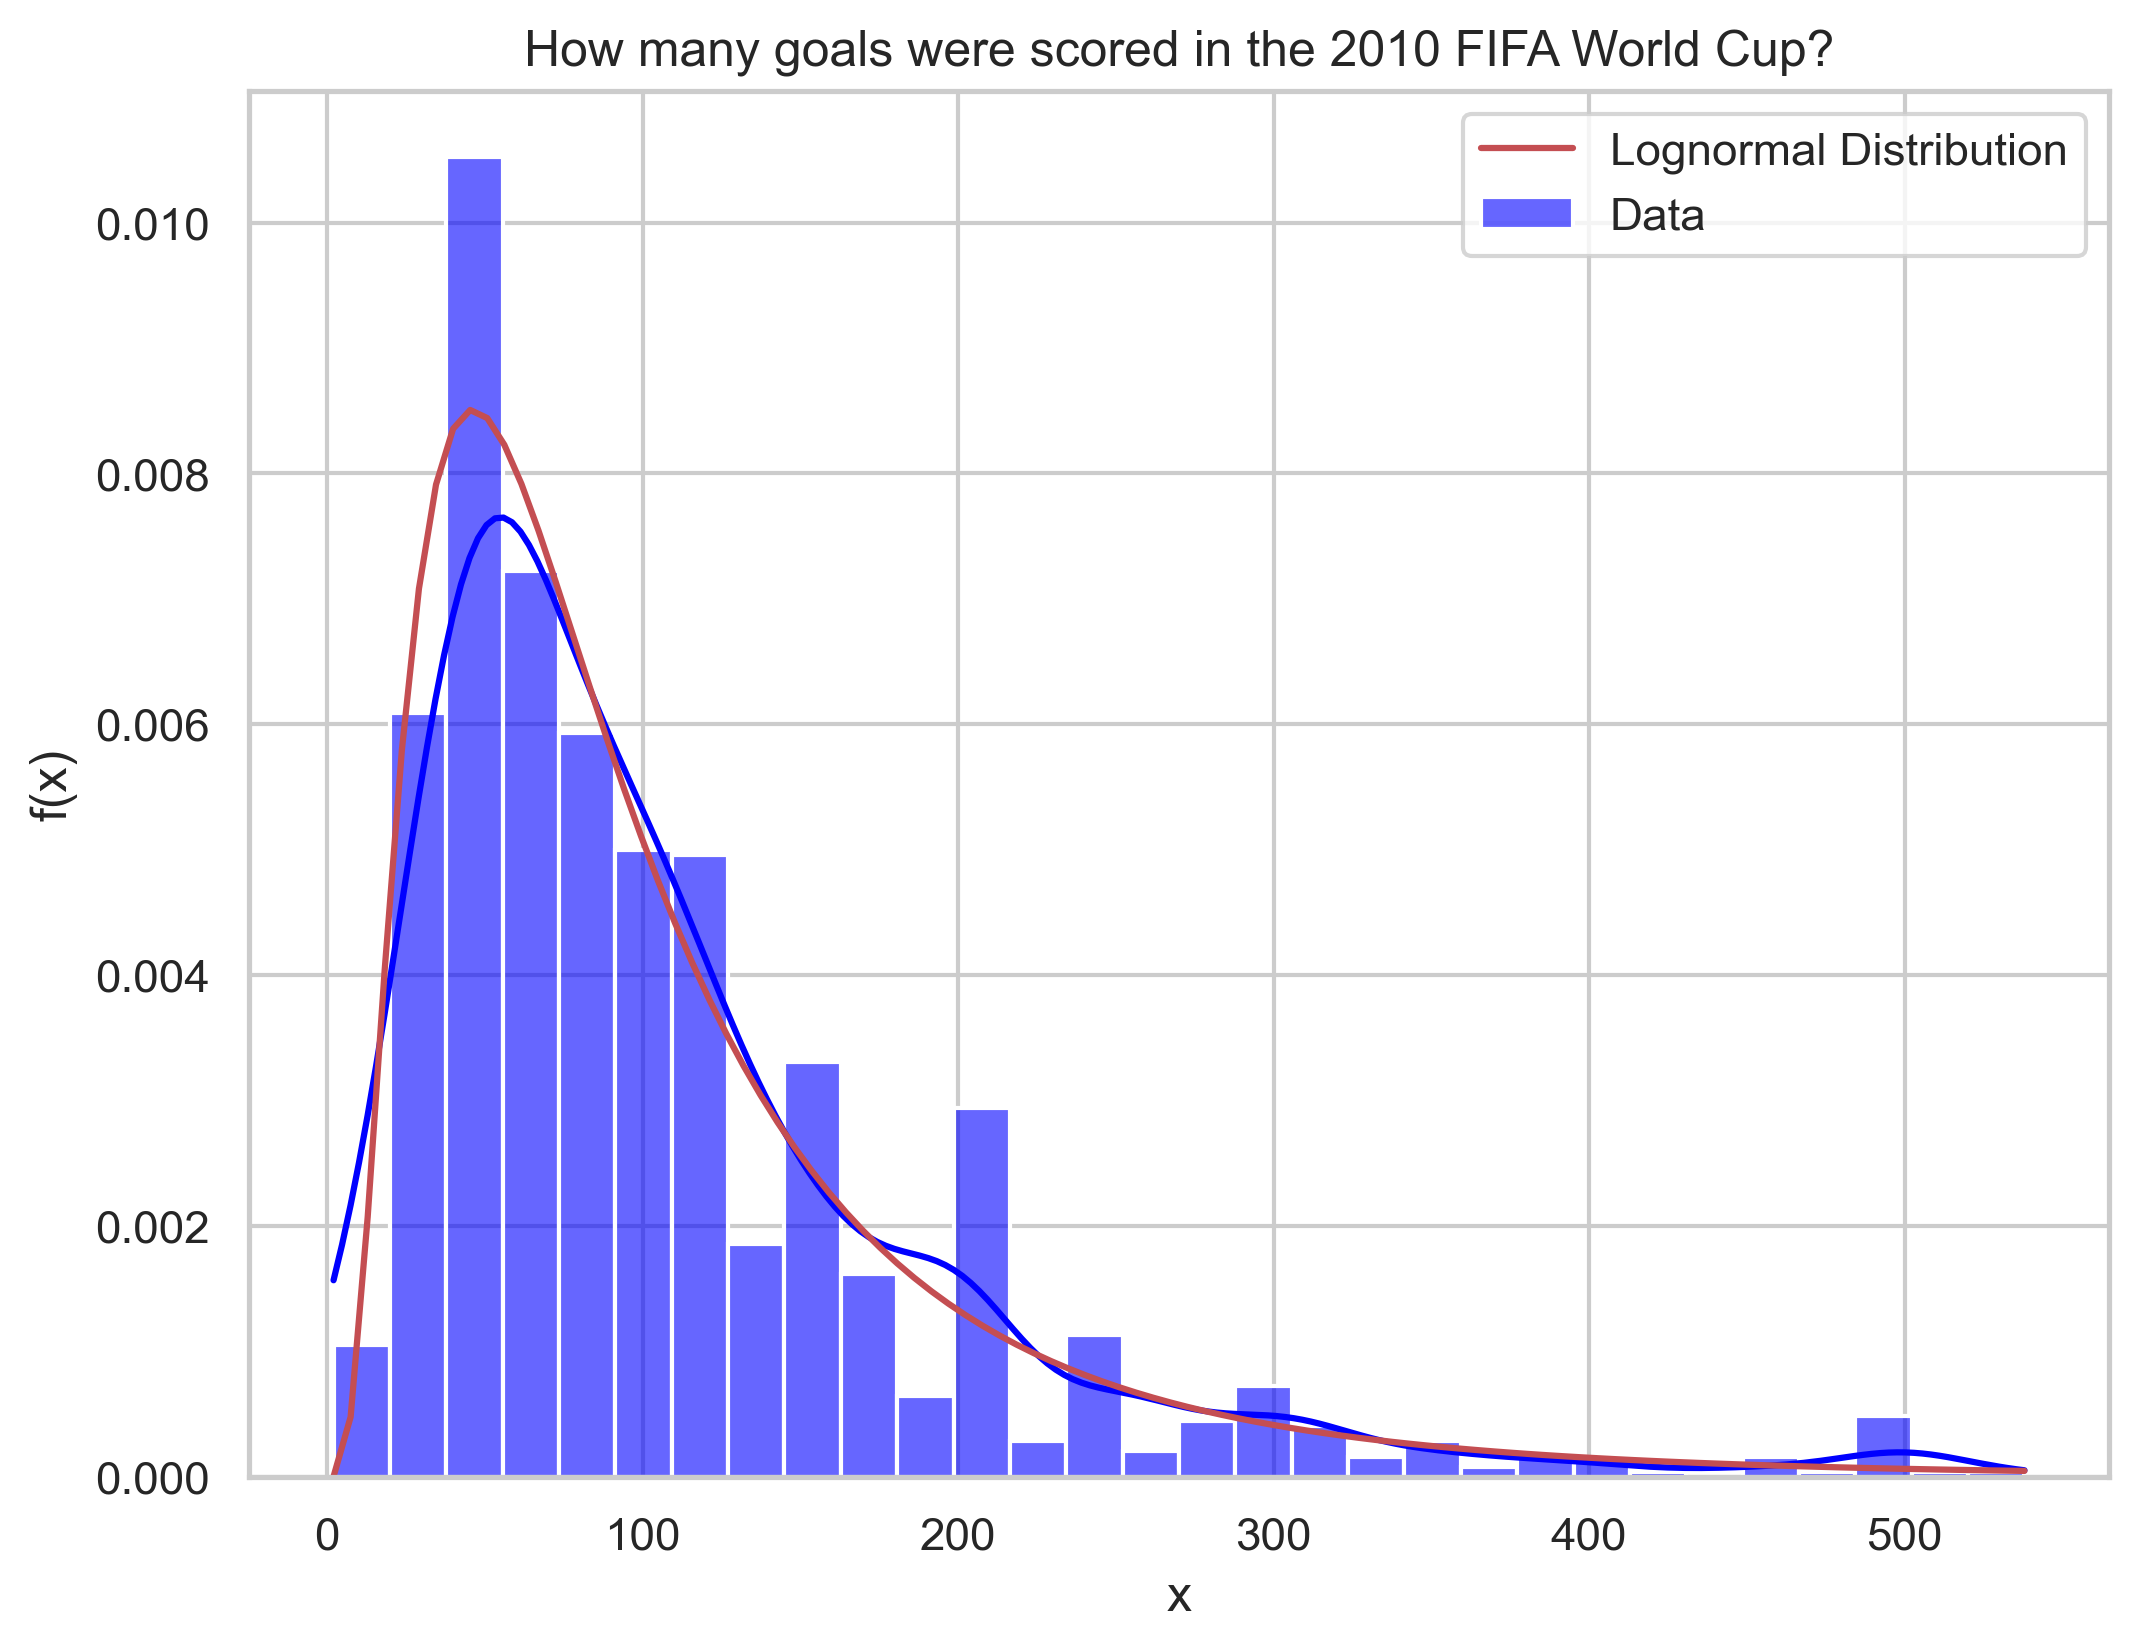
\includegraphics[width=0.8\textwidth]{figures/appendix_1/goals_distribution_log.png}
\caption{Distribución respuestas pregunta 1 y ajuste log-normal}
\end{figure}

\begin{figure}[h]
\centering
    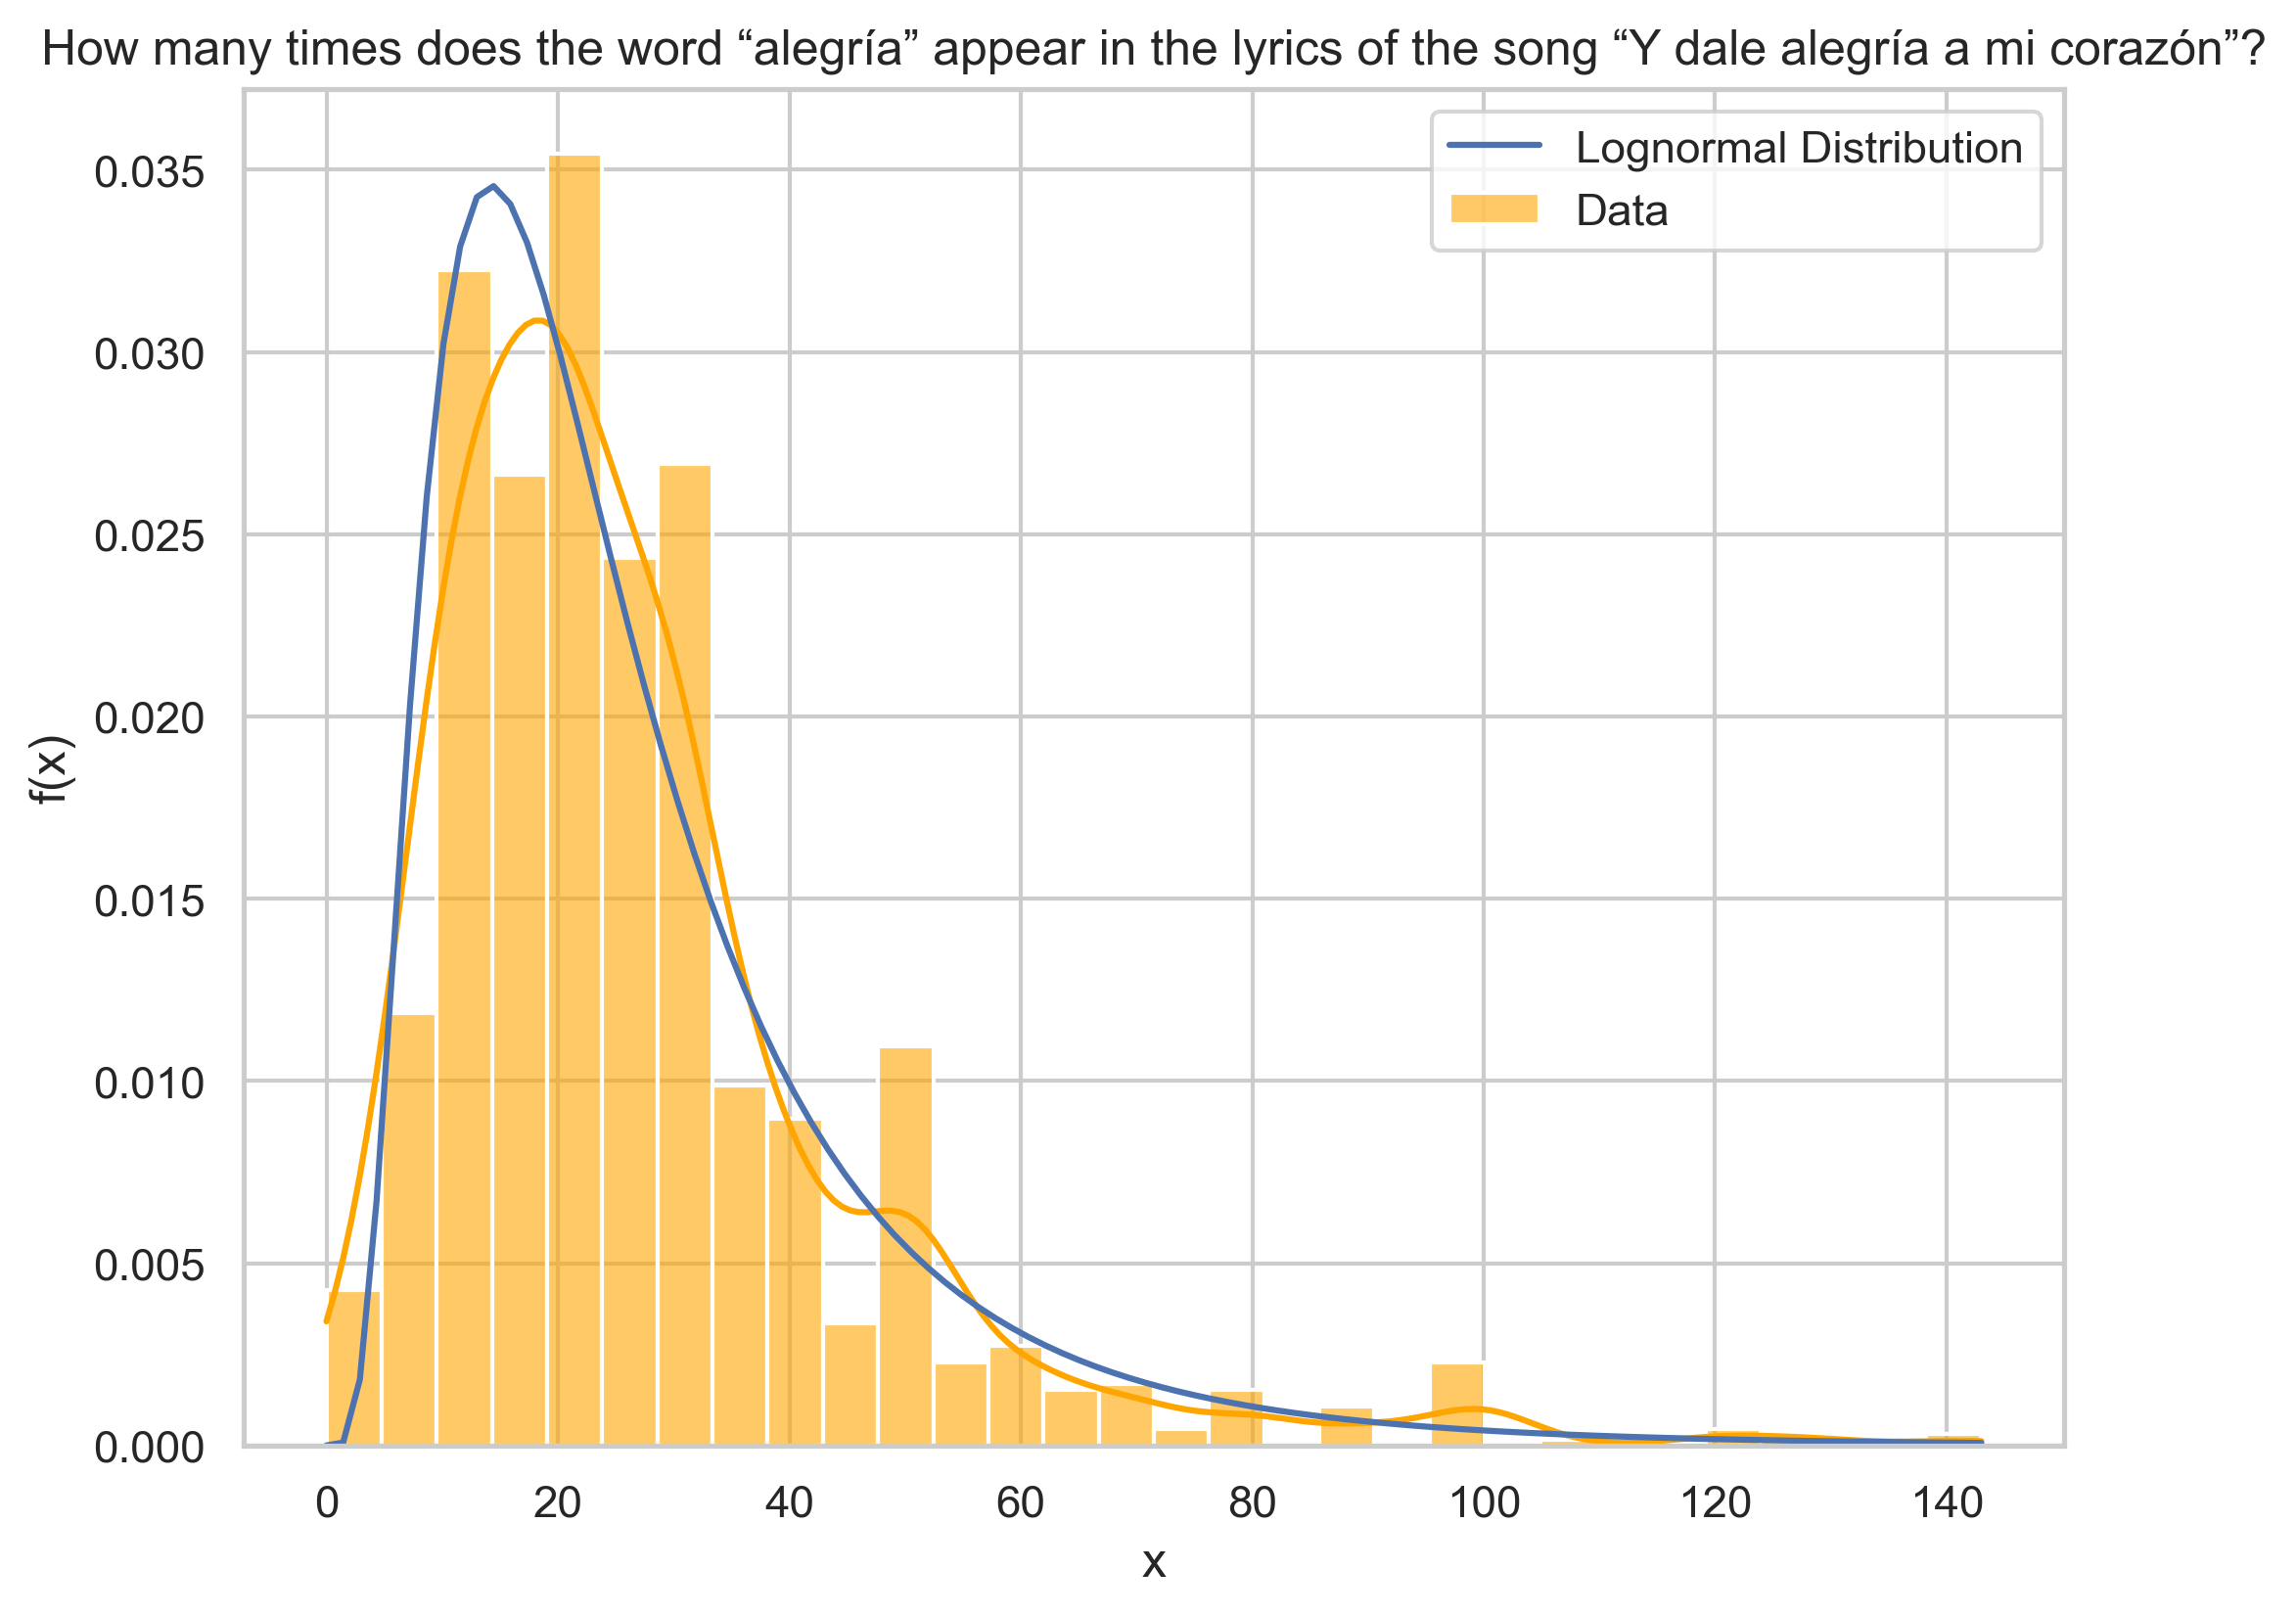
\includegraphics[width=0.8\textwidth]{figures/appendix_1/alegria_distribution_log.png}
\caption{Distribución respuestas pregunta 2 y ajuste log-normal}
\end{figure}

\begin{figure}[h]
\centering
    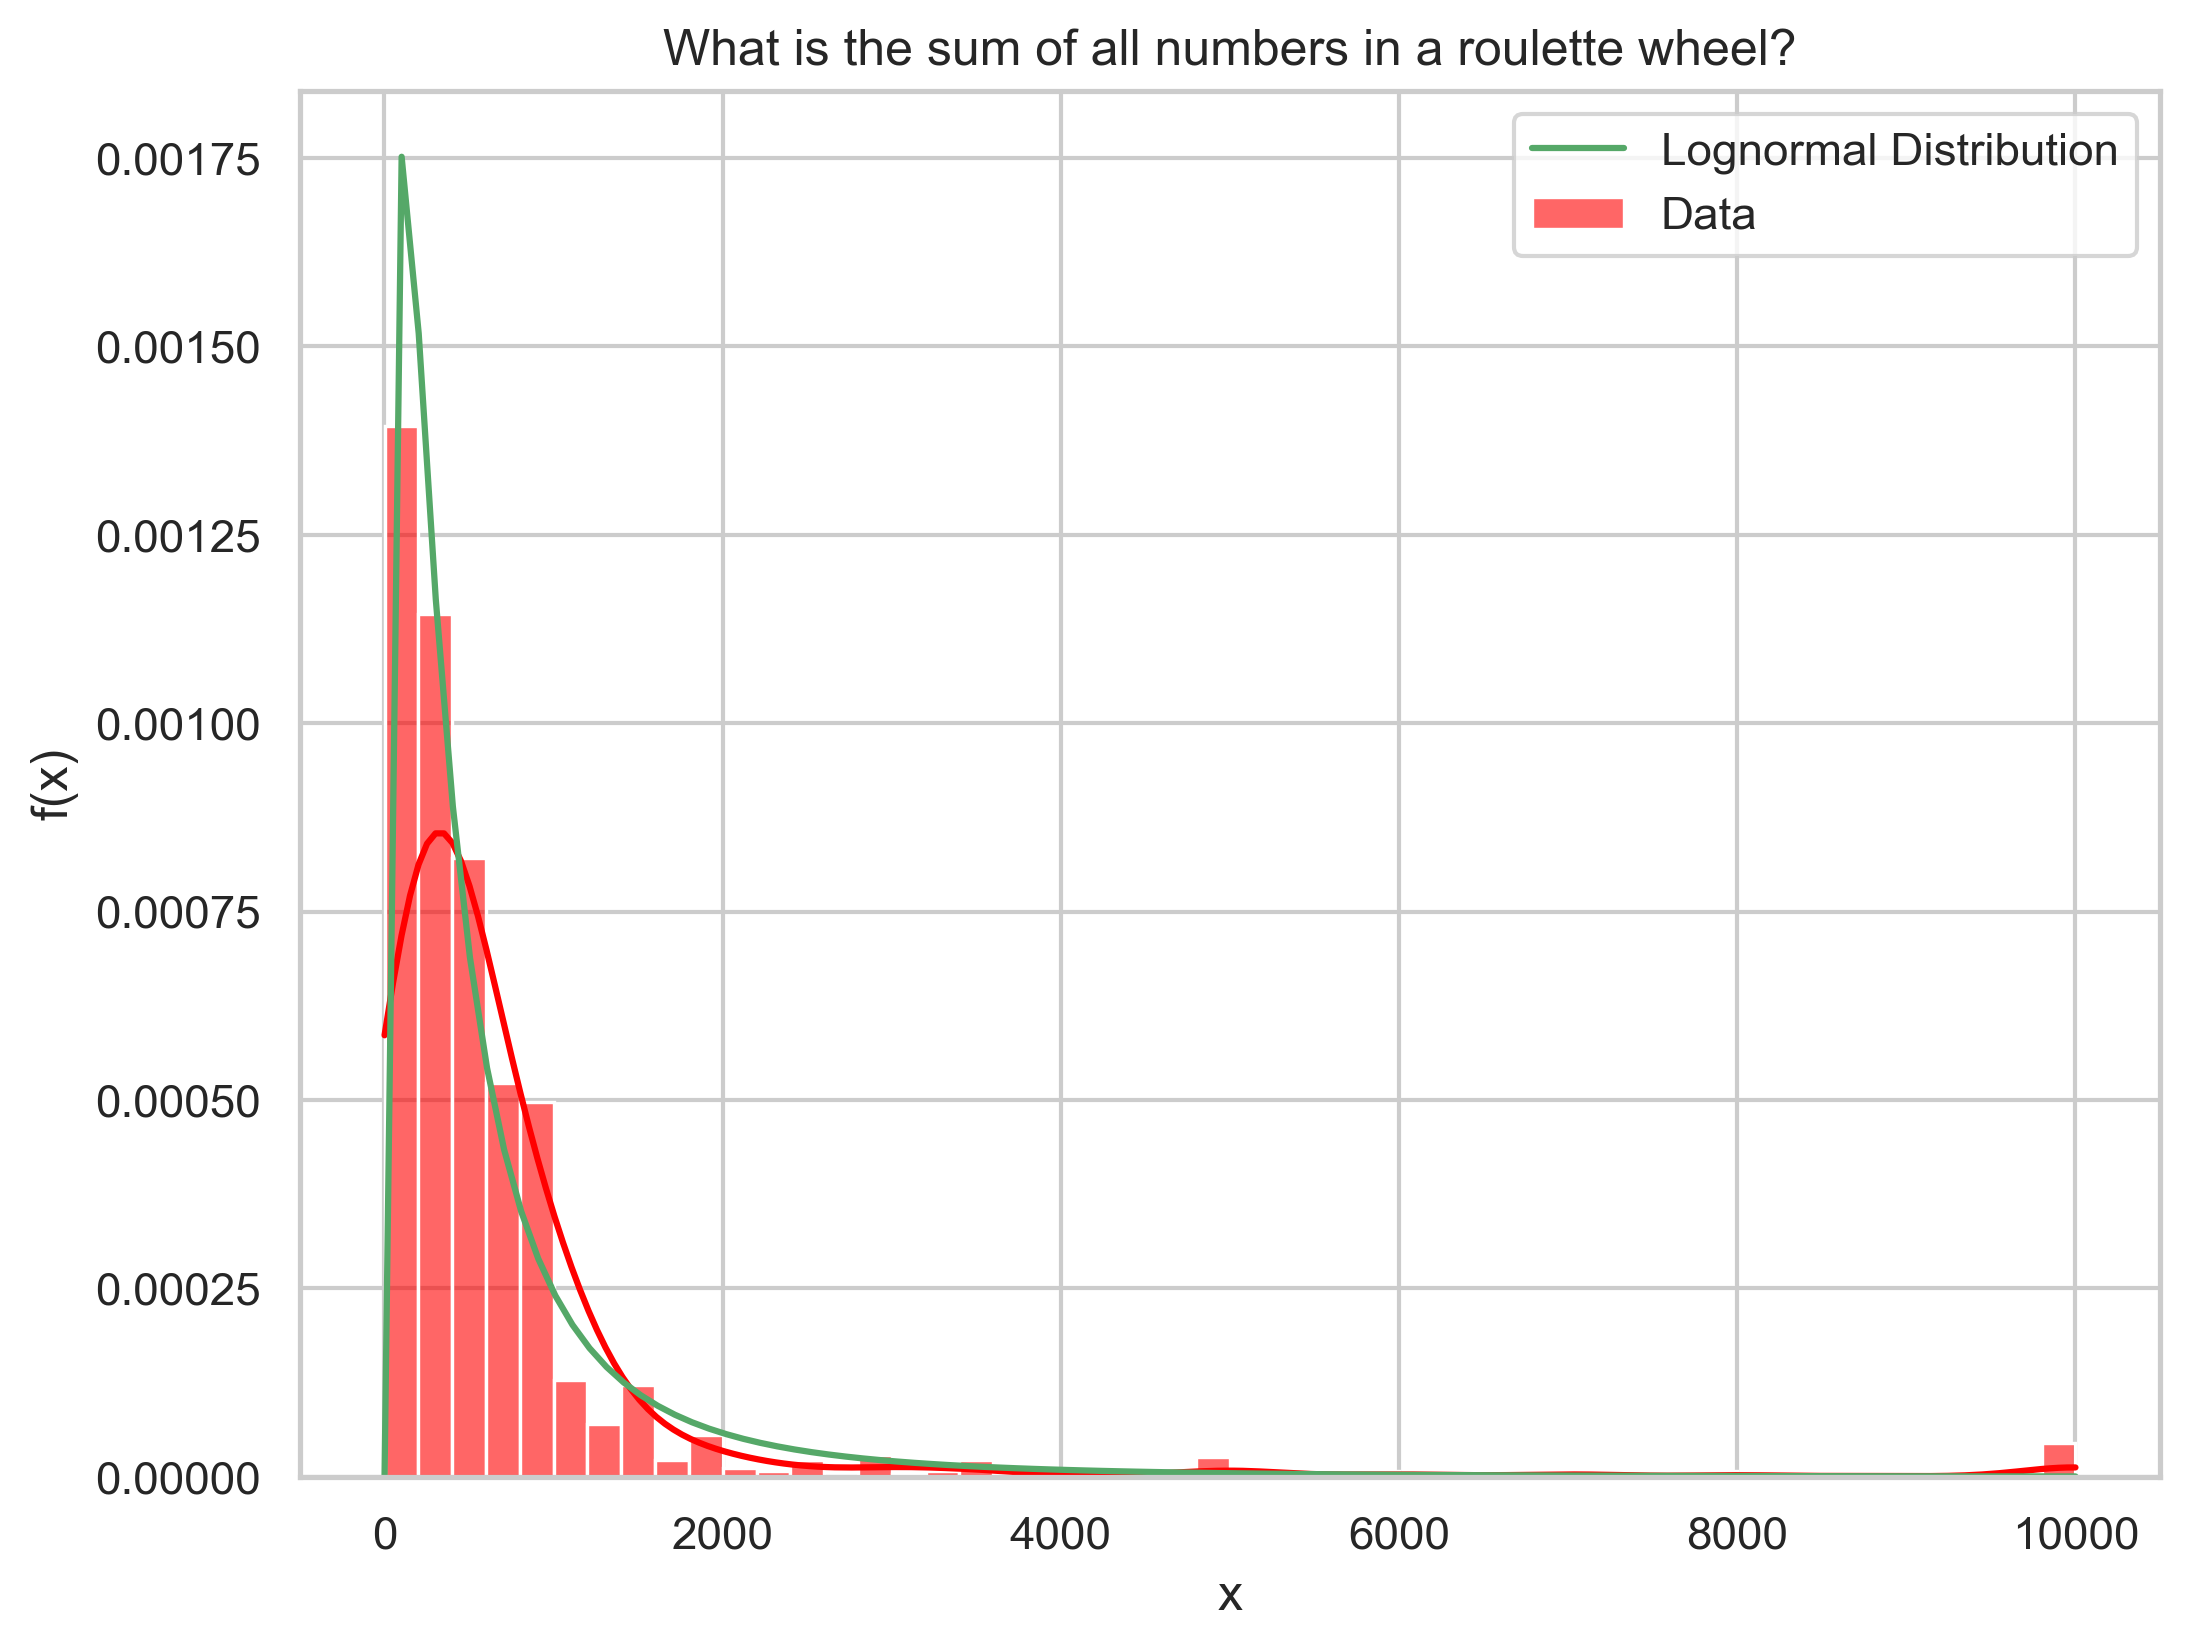
\includegraphics[width=0.8\textwidth]{figures/appendix_1/roullette_distribution_log.png}
\caption{Distribución respuestas pregunta 3 y ajuste log-normal}
\end{figure}

\begin{figure}[h]
\centering
    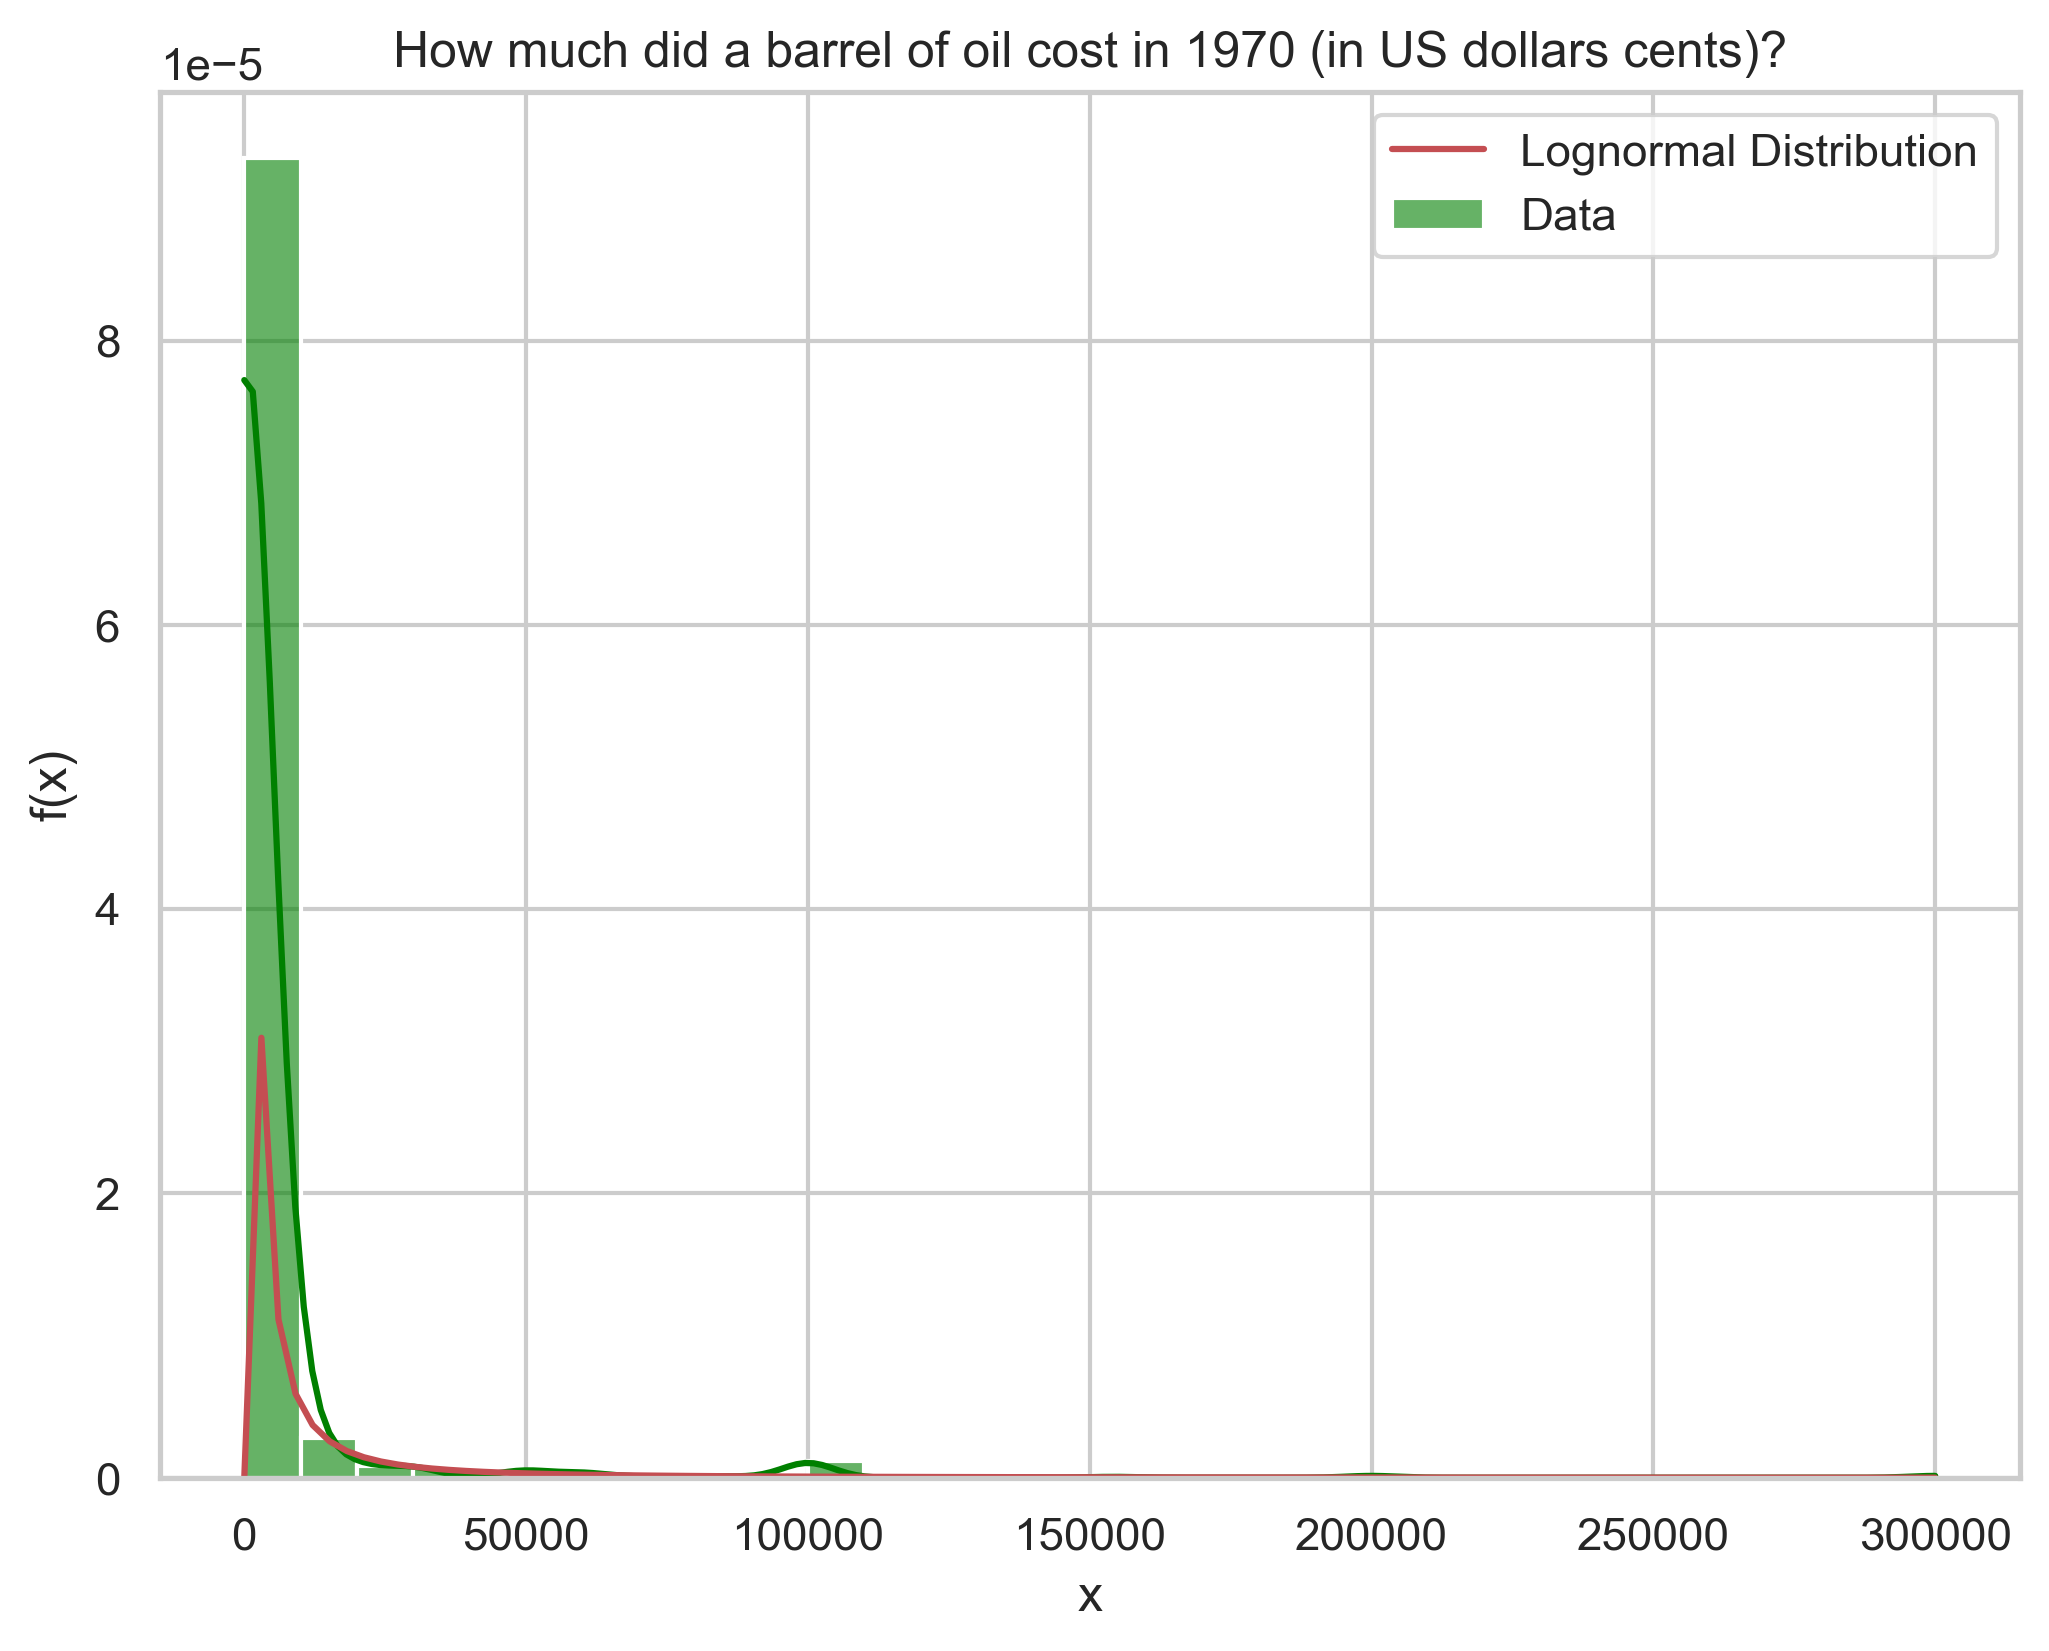
\includegraphics[width=0.8\textwidth]{figures/appendix_1/oil_distribution_log.png}
\caption{Distribución respuestas pregunta 4 y ajuste log-normal}
\end{figure}

% Ensure all figures are placed before moving to the next section
\FloatBarrier
 
\section*{2. Figuras distribución normal datos transformados}
 \label{appendix2}

 \begin{figure}[h]
\centering
    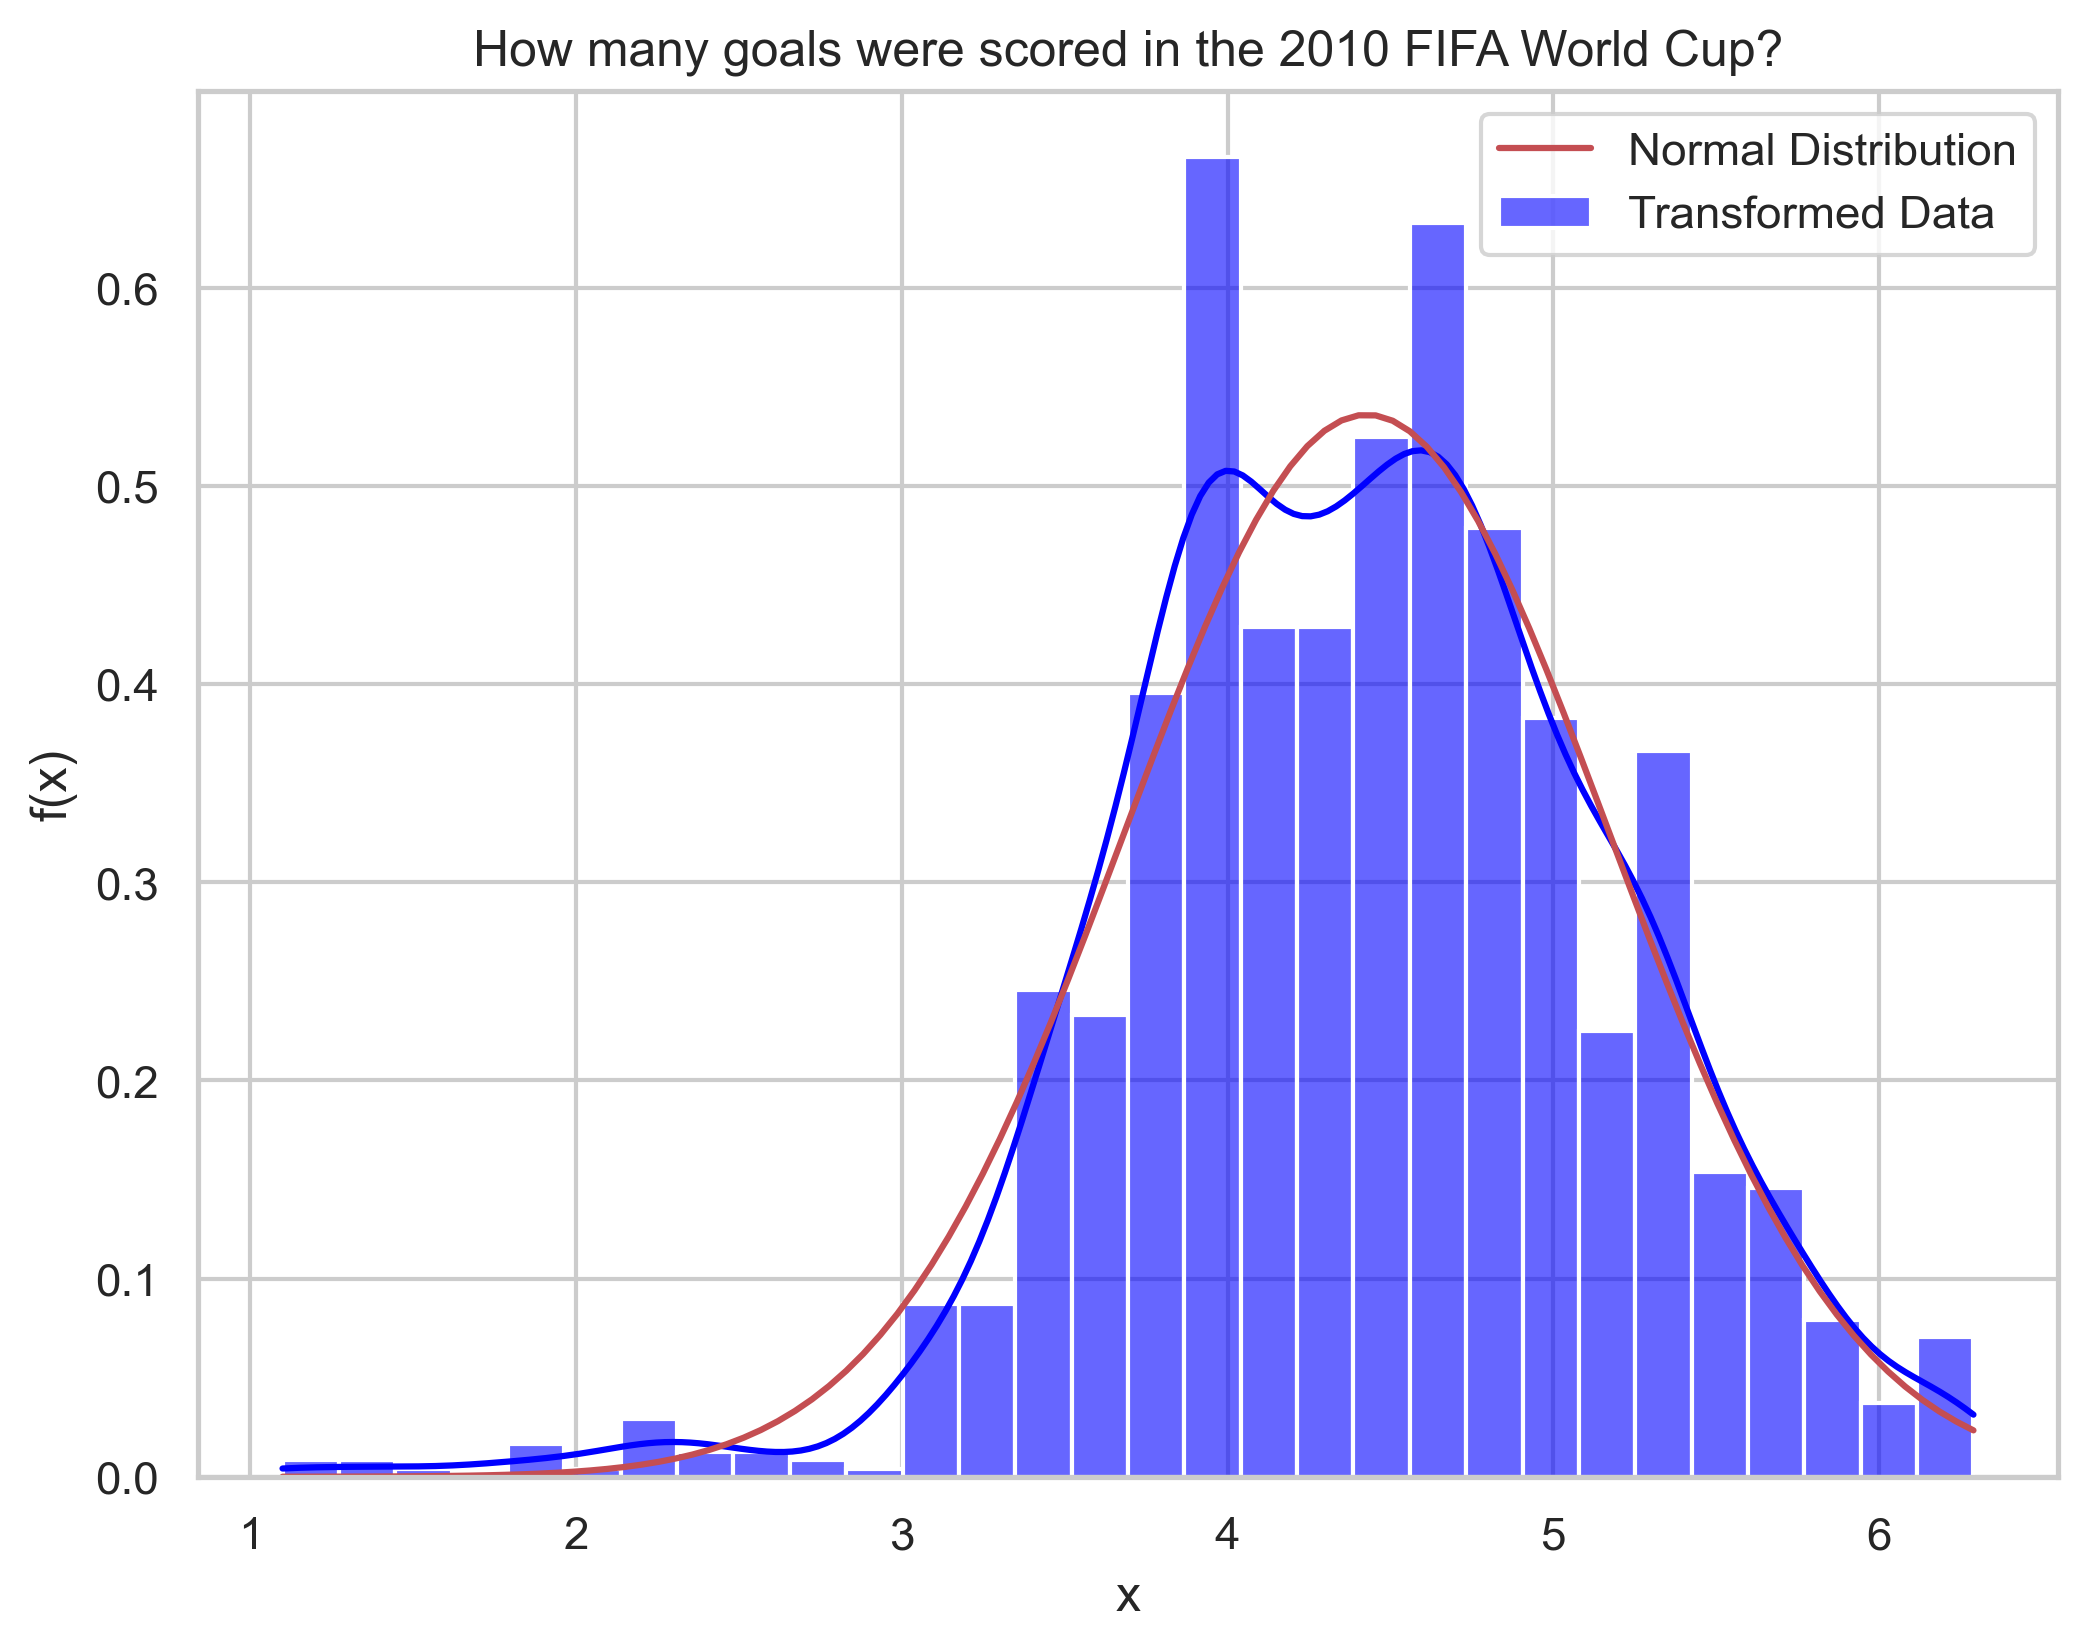
\includegraphics[width=0.8\textwidth]{figures/appendix_2/goals_distribution_normal.png}
\caption{Distribución respuestas pregunta 1 y ajuste normal}
\end{figure}

\begin{figure}[h]
\centering
    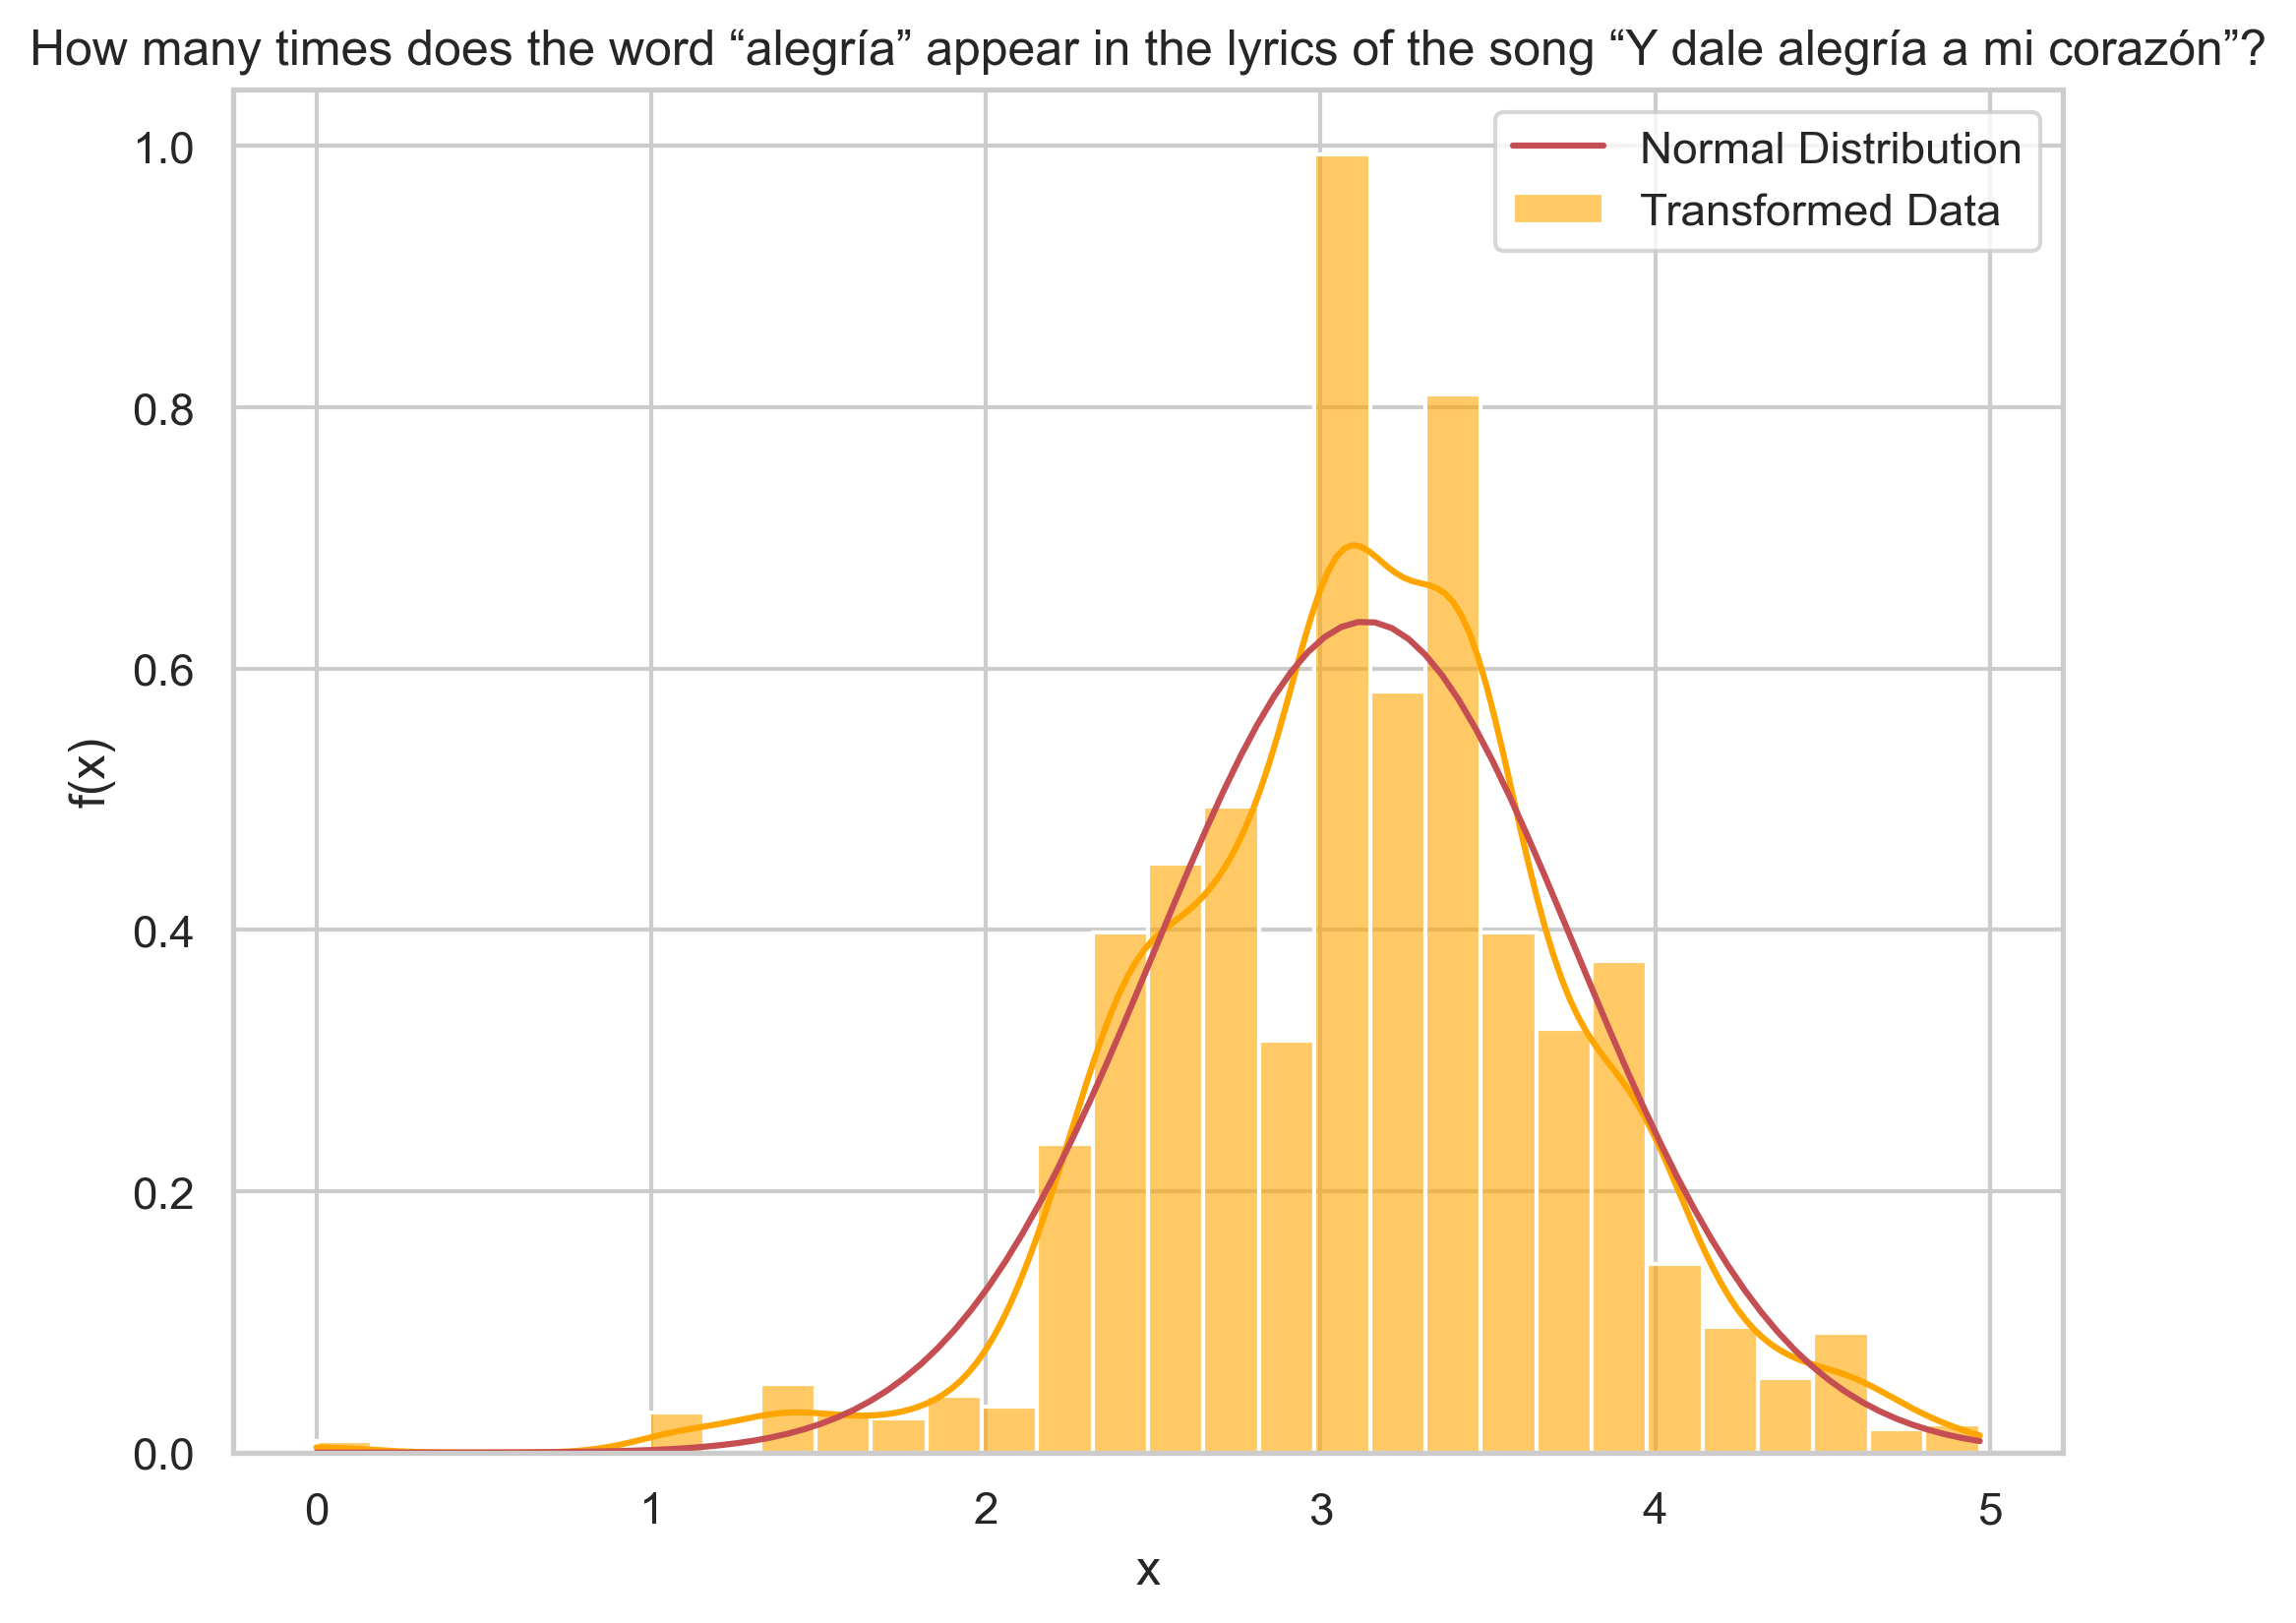
\includegraphics[width=0.8\textwidth]{figures/appendix_2/alegria_distribution_normal.png}
\caption{Distribución respuestas pregunta 2 y ajuste normal}
\end{figure}

\begin{figure}[h]
\centering
    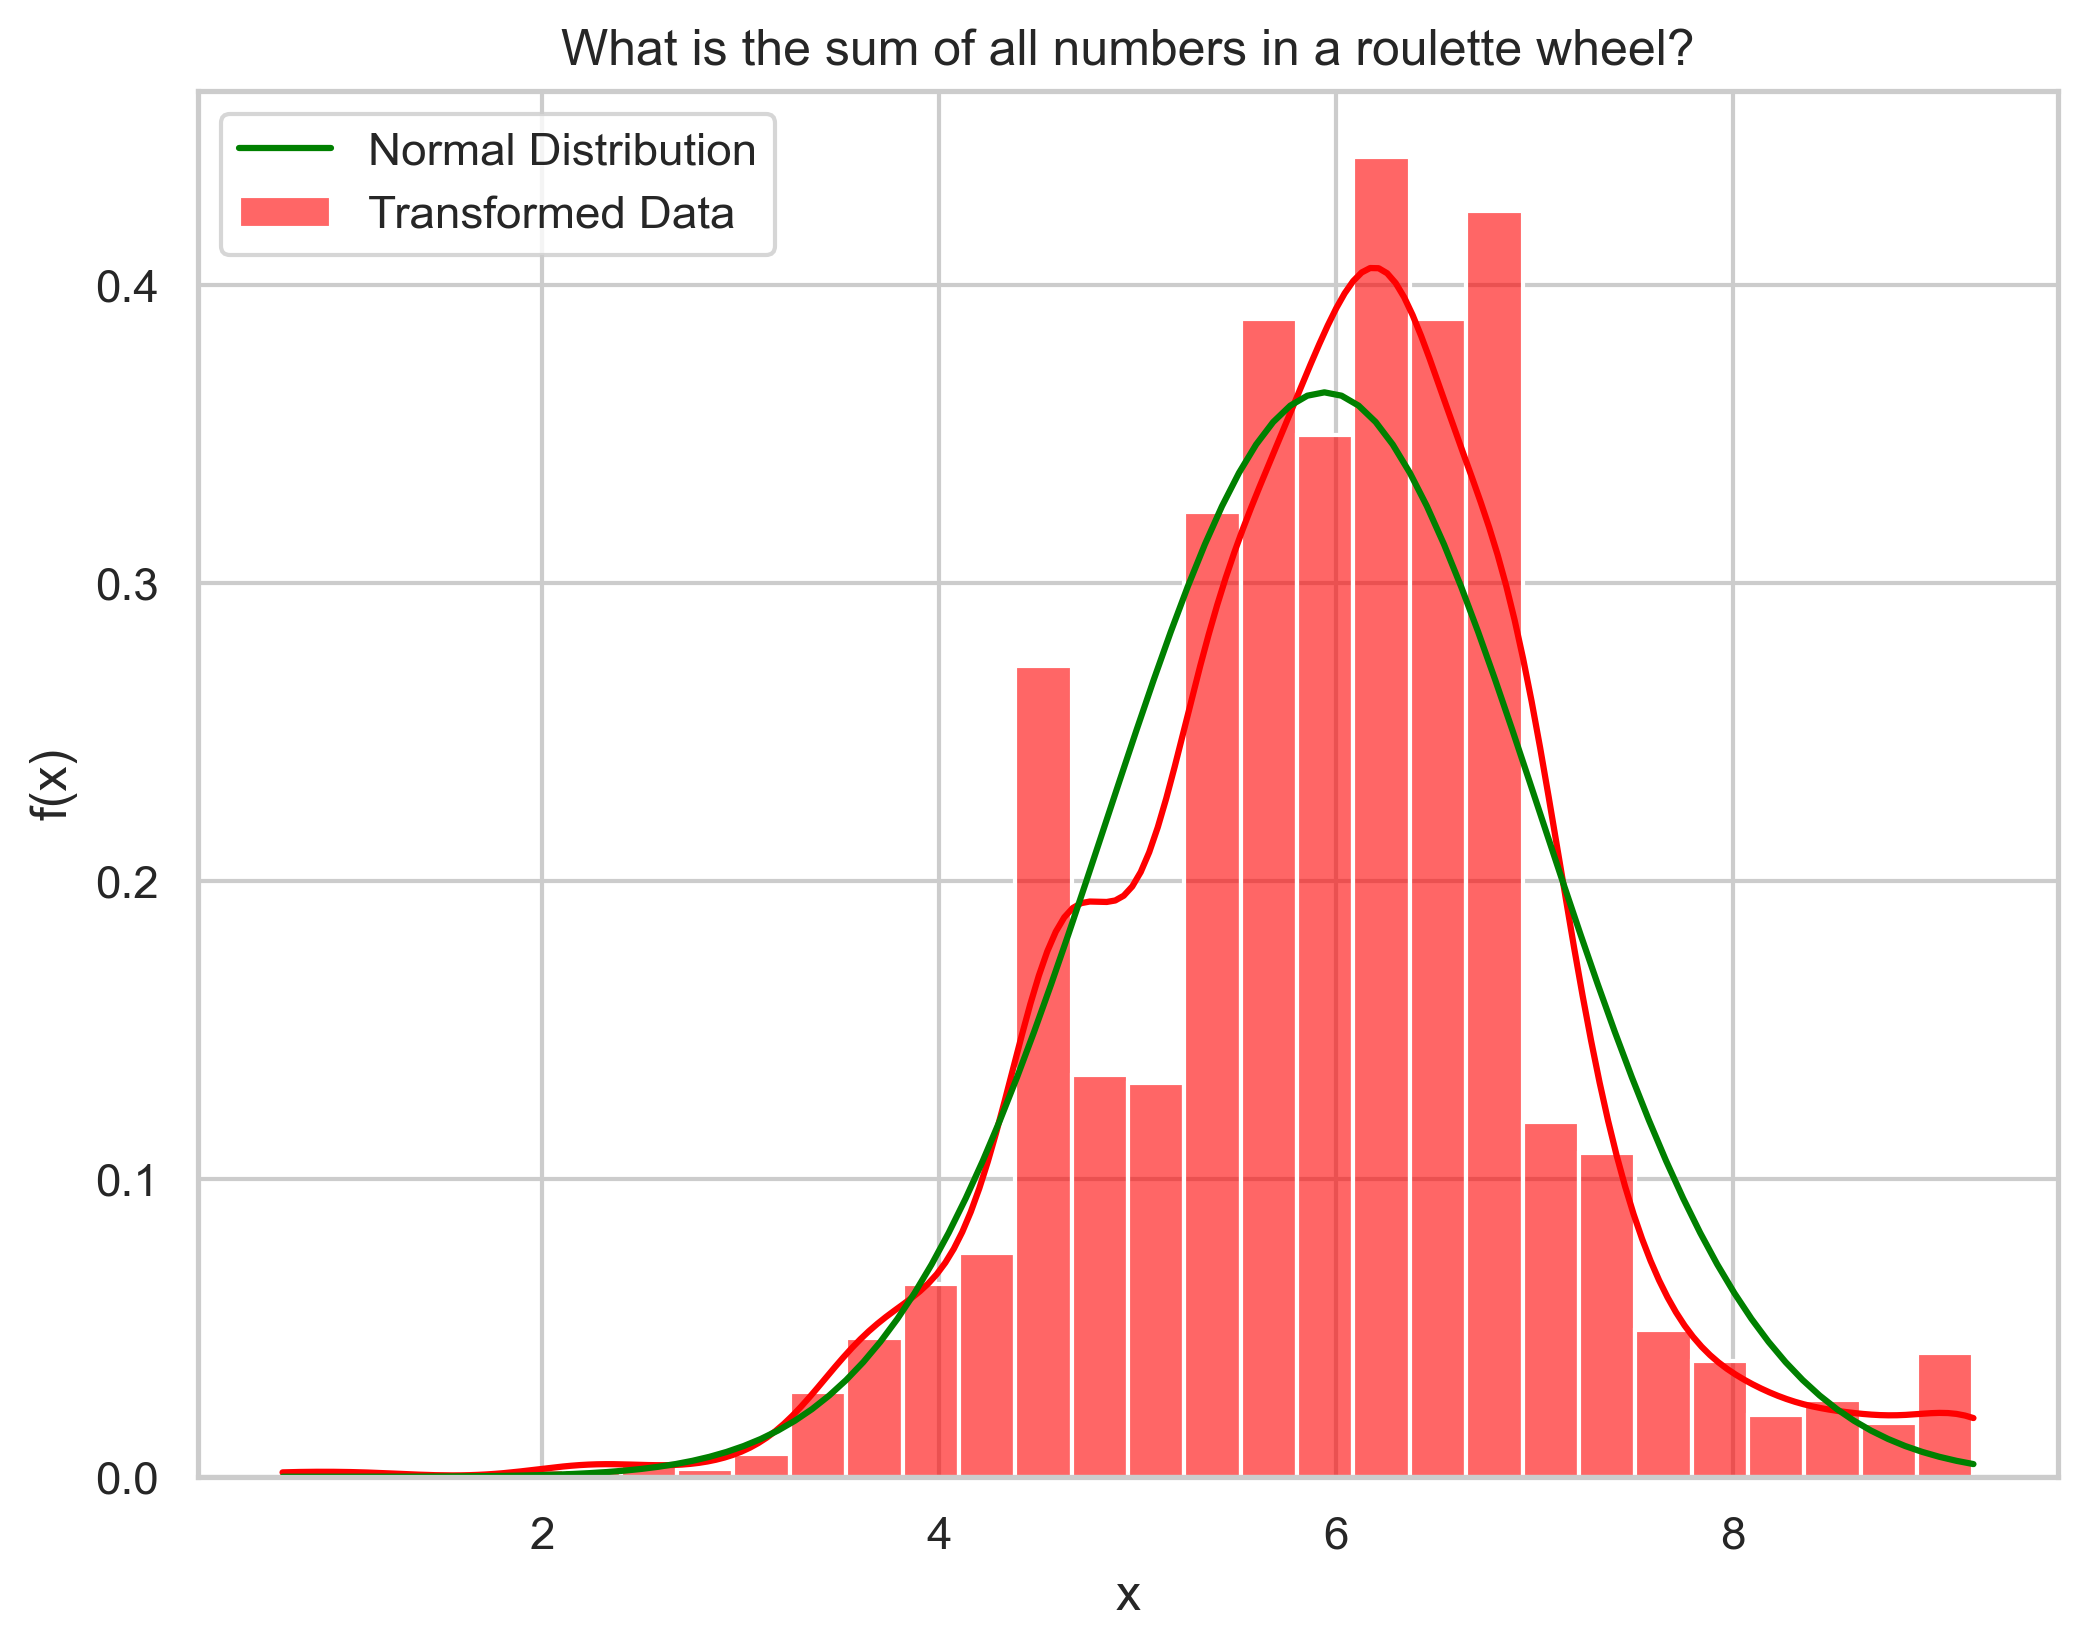
\includegraphics[width=0.8\textwidth]{figures/appendix_2/roullette_distribution_normal.png}
\caption{Distribución respuestas pregunta 3 y ajuste normal}
\end{figure}

\begin{figure}[h]
\centering
    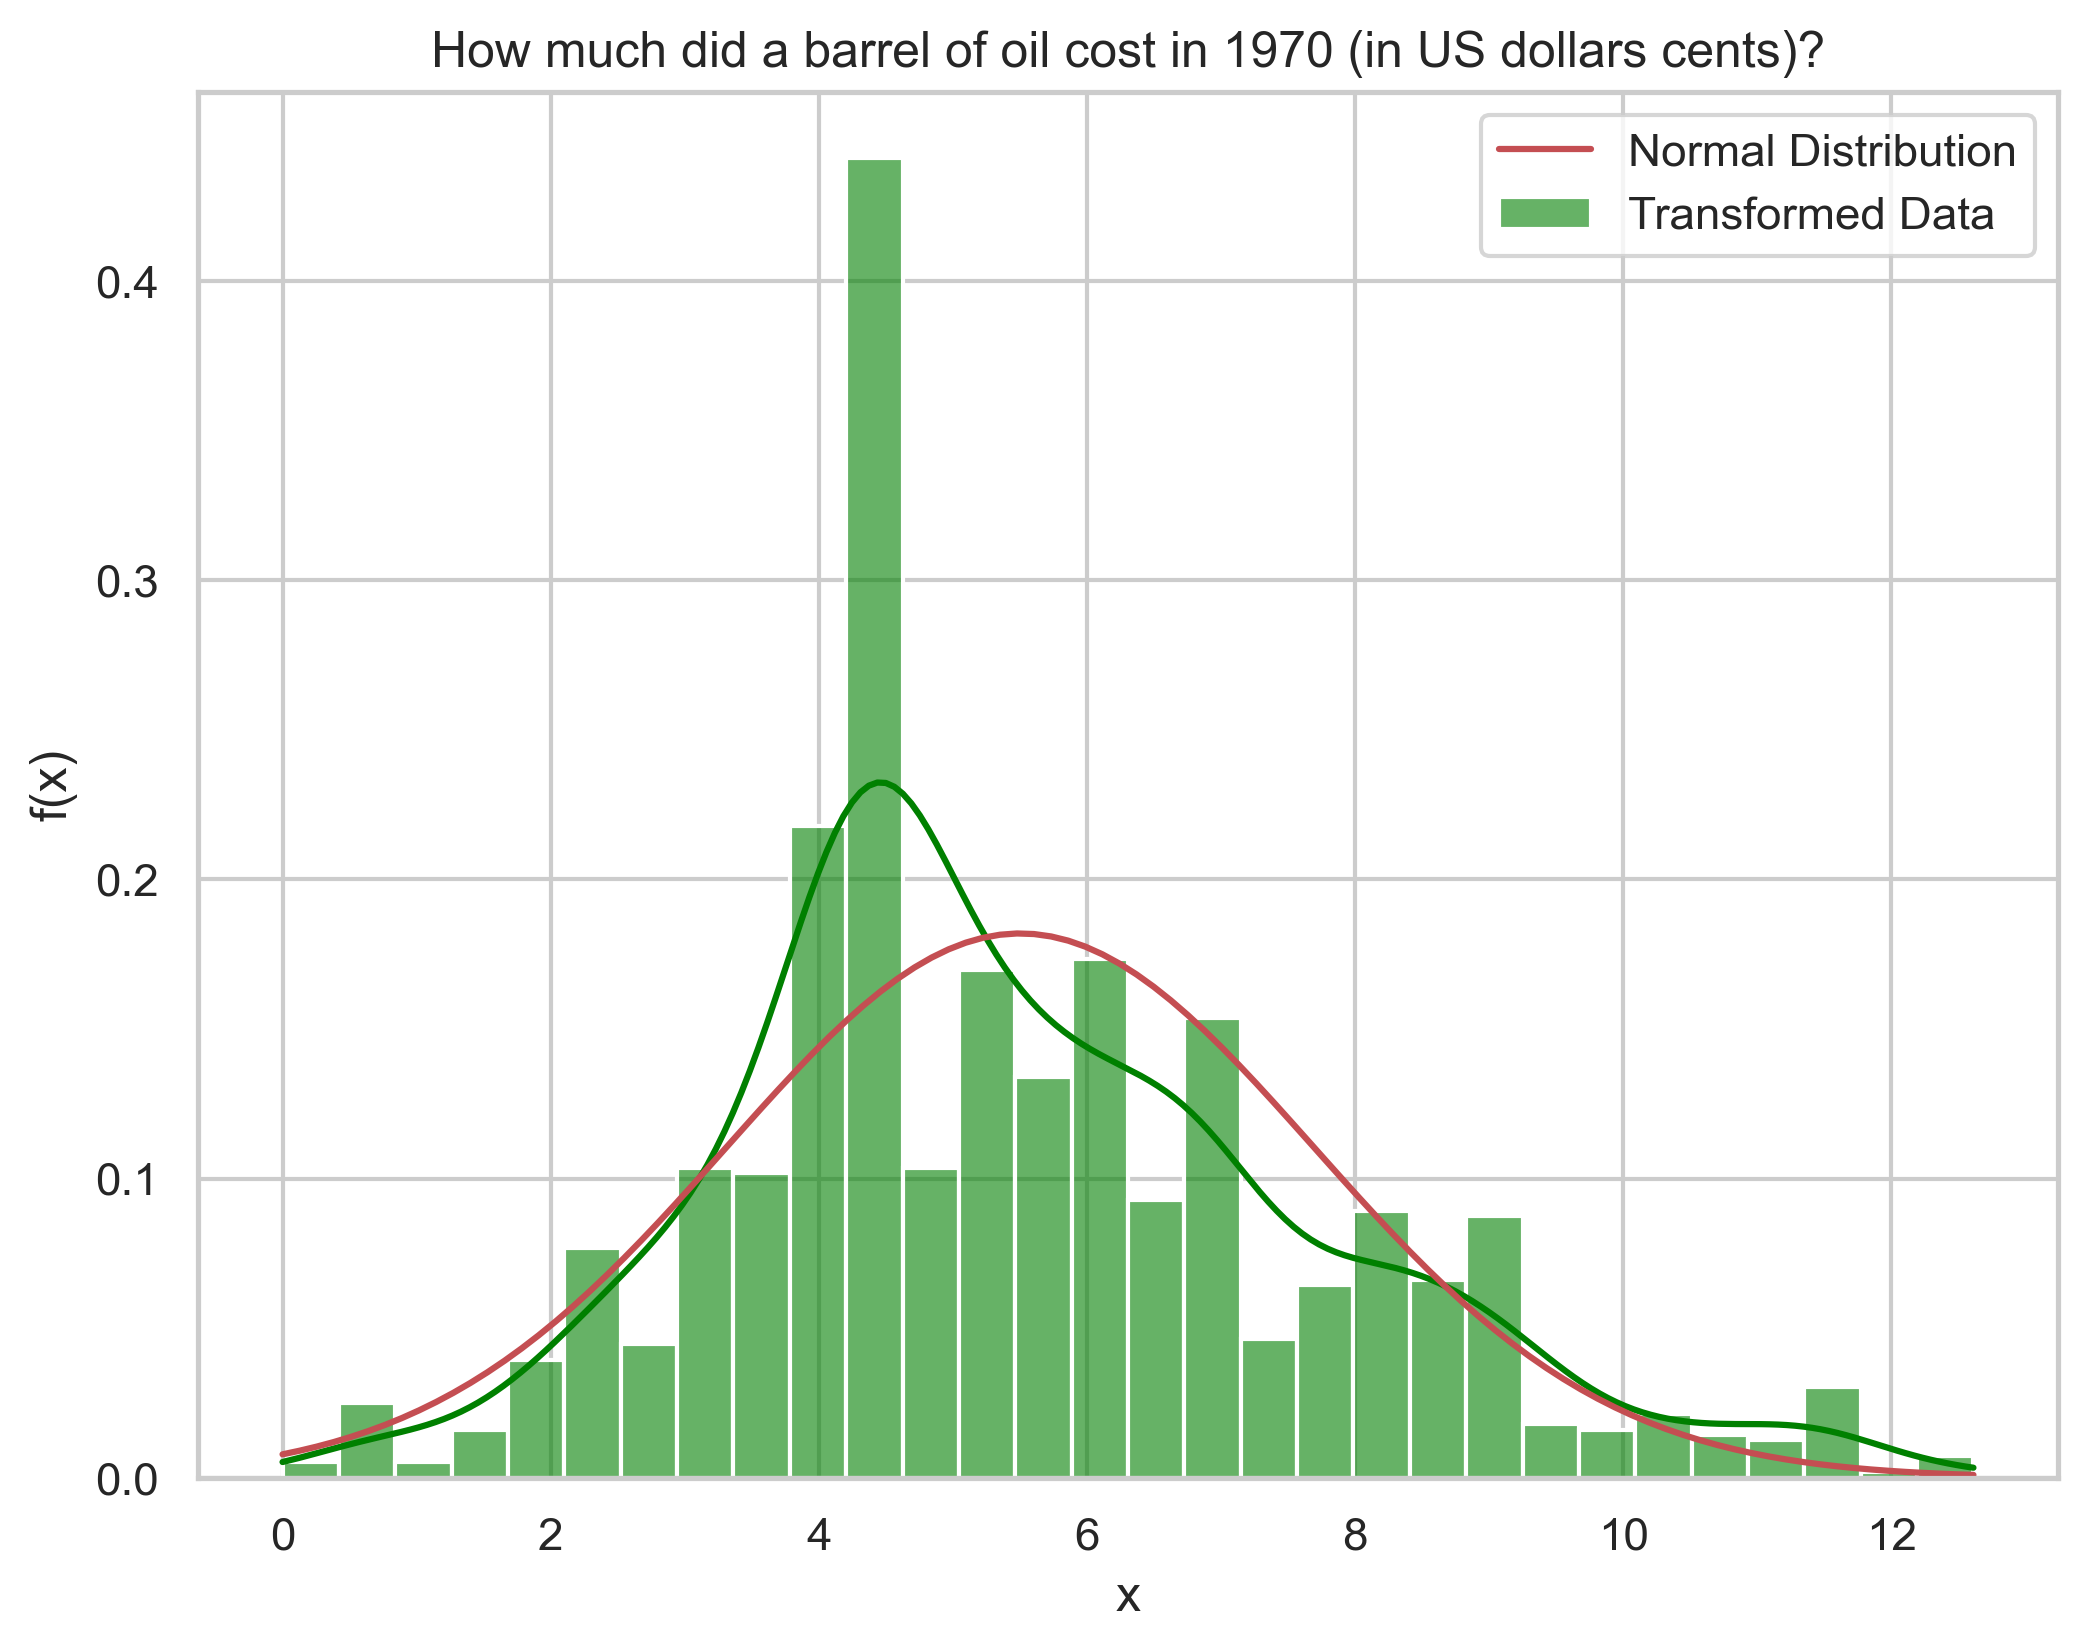
\includegraphics[width=0.8\textwidth]{figures/appendix_2/oil_distribution_normal.png}
\caption{Distribución respuestas pregunta 4 y ajuste normal}
\end{figure}

% Ensure all figures are placed before moving to the next section
\FloatBarrier
 
\section*{3. Tabla resultados test Shapiro-Wilk}
 \label{appendix3}
 
\begin{table}[h]
\centering
    \caption{Estadísticas y P-valores para diferentes preguntas}
    \label{tab:stats}
\begin{tabularx}{\textwidth}{l X X X}
\toprule
\textbf{Pregunta} & \textbf{Estadístico} & \textbf{P-valor} \\
\midrule
Goles    & $0.9839$ & $2.7140 \cdot 10^{-11}$ \\
Alegría  & $0.9833$ & $1.5691 \cdot 10^{-11}$ \\
Ruleta   & $0.9835$ & $2.5451 \cdot 10^{-11}$ \\
Petróleo & $0.9730$ & $4.7153 \cdot 10^{-15}$ \\
\bottomrule
\end{tabularx}
\end{table}

\FloatBarrier

\section*{4. Tabla datasets ordenados por nivel de aceptación}
 \label{appendix4}

\begin{table}[h]
\centering
    \caption{Proporción de aceptación de distribución por conjunto de datos}
\begin{tabularx}{\textwidth}{l X}
\toprule
\textbf{Nombre Dataset} & \textbf{Prop. aceptación} \\
\midrule
Carbon\_Emission.csv & 0.9485 \\
wind\_dataset.csv & 0.8360 \\
house\_8L.arff & 0.6954 \\
laptop.csv & 0.6143 \\
boston\_housing.arff & 0.5980 \\
abalone.csv & 0.5407 \\
salary\_football.csv & 0.4859 \\
Height.csv & 0.4171 \\
titanic\_fare.arff & 0.3817 \\
liver\_disorders.arff & 0.3623 \\
aerospace\_stock.arff & 0.3158 \\
Concrete\_Strength.csv & 0.3010 \\
kidney.arff & 0.25 \\
Metro\_Interstate\_Traffic\_Volume.csv & 0.2220 \\
weight.csv & 0.2098 \\
rainfall.arff & 0.1316 \\
flight\_price.csv & 0.1067 \\
medical\_costs.csv & 0.0784 \\
\bottomrule
\end{tabularx}
\end{table}

\FloatBarrier

\section*{5. Datasets seleccionados}
\label{appendix5}

Enlaces a los conjuntos de datos:

\begin{itemize}
    \item \href{https://www.openml.org/search?type=data&status=active&id=218}{House8L}
    \item \href{https://www.kaggle.com/datasets/fedesoriano/wind-speed-prediction-dataset}{Wind Speed}
    \item \href{https://www.kaggle.com/datasets/dumanmesut/individual-carbon-footprint-calculation}{Carbon Footprint}
    \item \href{https://www.kaggle.com/datasets/rodolfomendes/abalone-dataset}{Abalone}
    \item \href{https://www.openml.org/search?type=data&status=active&id=41539}{Rainfall}
    \item \href{https://www.kaggle.com/datasets/viveksharmar/flight-price-data}{Flight Price}
\end{itemize}

\section*{6. Setup entorno virtual}
\label{appendix6}

El paso por paso para configurar el entorno virtual se puede encontrar \textcolor{blue}{\href{https://github.com/fedeegiorgi/proyecto-final/blob/main/setup.pdf}{aquí}}.

\section*{7. Hiperparámetros definidos}
\label{appendix7}

\begin{table}[h]
\centering
    \caption{Hiperparámetros definidos para RF estándar por dataset.}
\begin{tabularx}{\textwidth}{l X}
\toprule
\textbf{Nombre Dataset} & \textbf{\texttt{max\_depth}} \\
\midrule
Carbon Footprint & 20 \\
House8L & 17 \\
Wind Speed & 12 \\
Abalone & 15 \\
Rainfall & 24 \\
Flight Price & 13 \\
\bottomrule
\end{tabularx}
\end{table}

\begin{table}[h]
\centering
    \caption{Hiperparámetros definidos para \texttt{IQRRandomForestRegressor} por dataset.}
\begin{tabularx}{\textwidth}{l X X X}
\toprule
\textbf{Nombre Dataset} & \textbf{\texttt{n\_estimators}} & \textbf{\texttt{group\_size}} & \textbf{\texttt{max\_depth}} \\
\midrule
Carbon Footprint & 150 & 3 & 20 \\
House8L & 150 & 3 & 32 \\
Wind Speed & 150 & 3 & 32 \\
Abalone & 150 & 3 & 12 \\
Rainfall & 150 & 3 & 21 \\
Flight Price & 150 & 3 & 13 \\
\bottomrule
\end{tabularx}
\end{table}

\begin{table}[h]
\centering
    \caption{Hiperparámetros definidos para \texttt{PercentileTrimmingRandomForestRegressor} por dataset.}
\begin{tabularx}{\textwidth}{l X X X X}
\toprule
\textbf{Nombre Dataset} & \textbf{\texttt{n\_estimators}} & \textbf{\texttt{group\_size}} & \textbf{\texttt{percentile}} &\textbf{\texttt{max\_depth}} \\
\midrule
Carbon Footprint & 150 & 50 & 2 & 44 \\
House8L & 150 & 50 & 2 & 40 \\
Wind Speed & 150 & 50 & 2 & 44 \\
Abalone & 150 & 50 & 2 & 12 \\
Rainfall & 150 & 50 & 2 & 23 \\
Flight Price & 150 & 50 & 2 & 13 \\
\bottomrule
\end{tabularx}
\end{table}

\begin{table}[h]
\centering
    \caption{Hiperparámetros definidos para \texttt{OOBRandomForestRegressor} por dataset.}
\begin{tabularx}{\textwidth}{l X X X}
\toprule
\textbf{Nombre Dataset} & \textbf{\texttt{n\_estimators}} & \textbf{\texttt{group\_size}} & \textbf{\texttt{max\_depth}} \\
\midrule
Carbon Footprint & 180 & 3 & 17 \\
House8L & 180 & 3 & 17 \\
Wind Speed & 180 & 3 & 19 \\
Abalone & 180 & 3 & 10 \\
Rainfall & 180 & 3 & 23 \\
Flight Price & 180 & 3 & 13 \\
\bottomrule
\end{tabularx}
\end{table}

\begin{table}[h]
\centering
    \caption{Hiperparámetros definidos para \texttt{OOBPlusIQRRandomForestRegressor} por dataset.}
\begin{tabularx}{\textwidth}{l X X X}
\toprule
\textbf{Nombre Dataset} & \textbf{\texttt{n\_estimators}} & \textbf{\texttt{group\_size}} & \textbf{\texttt{max\_depth}} \\
\midrule
Carbon Footprint & 180 & 3 & 21 \\
House8L & 180 & 3 & 42 \\
Wind Speed & 180 & 3 & 14 \\
Abalone & 180 & 3 & 10 \\
Rainfall & 180 & 3 & 23 \\
Flight Price & 180 & 3 & 13 \\
\bottomrule
\end{tabularx}
\end{table}

\begin{table}[h]
\centering
    \caption{Hiperparámetros definidos para \texttt{FirstSplitCombinerRandomForestRegressor} por dataset.}
\begin{tabularx}{\textwidth}{l X X X}
\toprule
\textbf{Nombre Dataset} & \textbf{\texttt{n\_estimators}} & \textbf{\texttt{group\_size}} & \textbf{\texttt{max\_features}} \\
\midrule
Carbon Footprint & 100 & 10 & $log_2$ \\
House8L & 100 & 10 & $log_2$ \\
Wind Speed & 100 & 10 & $log_2$ \\
Abalone & 100 & 10 & $log_2$ \\
Rainfall & 100 & 10 & $log_2$ \\
Flight Price & 100 & 10 & $log_2$ \\
\bottomrule
\end{tabularx}
\end{table}

\begin{table}[h]
\centering
    \caption{Hiperparámetros definidos para \texttt{SharedKnowledgeRandomForestRegressor} por dataset.}
\begin{tabularx}{\textwidth}{l X X X X}
\toprule
\textbf{Nombre Dataset} & \textbf{\texttt{n\_estimators}} & \textbf{\texttt{group\_size}} & \textbf{\texttt{initial\_max\_depth}} &\textbf{\texttt{max\_depth}} \\
\midrule
Carbon Footprint & 280 & 7 & 14 & 20 \\
House8L & 280 & 7 & 14 & 23 \\
Wind Speed & 280 & 7 & 14 & 25 \\
Abalone & 280 & 7 & 14 & 23 \\
Rainfall & 280 & 7 & 14 & 39 \\
Flight Price & 280 & 7 & 14 & 20 \\
\bottomrule
\end{tabularx}
\end{table}

\FloatBarrier

\section*{8. Tablas comparación de modelos cross-validation}
\label{appendix8}

\begin{table}[h]
\centering
\begin{tabular}{|l|c|c|c|}
\hline
Model & Fold & MSE & Rank \\ \hline
\textcolor[HTML]{b33dc6}{OOBRandomForestRegressor} & 6 & 219626.05 & 1 \\ \hline
\textcolor[HTML]{ede15b}{OOBPlusIQRRandomForestRegressor} & 6 & 220018.76 & 2 \\ \hline
\textcolor[HTML]{27aeef}{IQRRandomForestRegressor} & 6 & 221685.1 & 3 \\ \hline
\textcolor[HTML]{ef9b20}{SharedKnowledgeRandomForestRegressor} & 6 & 221735.16 & 4 \\ \hline
\textcolor[HTML]{f46a9b}{PercentileTrimmingRandomForestRegressor} & 6 & 223235.21 & 5 \\ \hline
\textcolor[HTML]{f46a9b}{PercentileTrimmingRandomForestRegressor} & 3 & 223237.69 & 6 \\ \hline
\textcolor[HTML]{87bc45}{RandomForestRegressor} & 6 & 223837.16 & 7 \\ \hline
\textcolor[HTML]{27aeef}{IQRRandomForestRegressor} & 3 & 223963.58 & 8 \\ \hline
\textcolor[HTML]{87bc45}{RandomForestRegressor} & 3 & 224435.49 & 9 \\ \hline
\textcolor[HTML]{ede15b}{OOBPlusIQRRandomForestRegressor} & 3 & 224960.73 & 10 \\ \hline
\textcolor[HTML]{b33dc6}{OOBRandomForestRegressor} & 3 & 225963.59 & 11 \\ \hline
\textcolor[HTML]{b33dc6}{OOBRandomForestRegressor} & 1 & 226485.15 & 12 \\ \hline
\textcolor[HTML]{ef9b20}{SharedKnowledgeRandomForestRegressor} & 1 & 227177.42 & 13 \\ \hline
\textcolor[HTML]{87bc45}{RandomForestRegressor} & 1 & 227370.46 & 14 \\ \hline
\textcolor[HTML]{ef9b20}{SharedKnowledgeRandomForestRegressor} & 3 & 227639.59 & 15 \\ \hline
\textcolor[HTML]{ede15b}{OOBPlusIQRRandomForestRegressor} & 1 & 230364.45 & 16 \\ \hline
\textcolor[HTML]{27aeef}{IQRRandomForestRegressor} & 1 & 231118.59 & 17 \\ \hline
\textcolor[HTML]{f46a9b}{PercentileTrimmingRandomForestRegressor} & 1 & 231349.01 & 18 \\ \hline
\textcolor[HTML]{ede15b}{OOBPlusIQRRandomForestRegressor} & 7 & 234270.29 & 19 \\ \hline
\textcolor[HTML]{ef9b20}{SharedKnowledgeRandomForestRegressor} & 7 & 234414.21 & 20 \\ \hline
\textcolor[HTML]{27aeef}{IQRRandomForestRegressor} & 7 & 235863.45 & 21 \\ \hline
\textcolor[HTML]{b33dc6}{OOBRandomForestRegressor} & 7 & 237262.67 & 22 \\ \hline
\textcolor[HTML]{f46a9b}{PercentileTrimmingRandomForestRegressor} & 7 & 238727.65 & 23 \\ \hline
\textcolor[HTML]{87bc45}{RandomForestRegressor} & 7 & 239410.77 & 24 \\ \hline
\textcolor[HTML]{87bc45}{RandomForestRegressor} & 10 & 265857.34 & 25 \\ \hline
\textcolor[HTML]{f46a9b}{PercentileTrimmingRandomForestRegressor} & 10 & 266813.52 & 26 \\ \hline
\textcolor[HTML]{ef9b20}{SharedKnowledgeRandomForestRegressor} & 10 & 269693.51 & 27 \\ \hline
\textcolor[HTML]{ede15b}{OOBPlusIQRRandomForestRegressor} & 5 & 270346.36 & 28 \\ \hline
\textcolor[HTML]{b33dc6}{OOBRandomForestRegressor} & 5 & 270553.23 & 29 \\ \hline
\textcolor[HTML]{ef9b20}{SharedKnowledgeRandomForestRegressor} & 5 & 270889.04 & 30 \\ \hline
\textcolor[HTML]{ede15b}{OOBPlusIQRRandomForestRegressor} & 10 & 271041.6 & 31 \\ \hline
\textcolor[HTML]{87bc45}{RandomForestRegressor} & 5 & 272362.94 & 32 \\ \hline
\textcolor[HTML]{27aeef}{IQRRandomForestRegressor} & 5 & 272471.19 & 33 \\ \hline
\textcolor[HTML]{b33dc6}{OOBRandomForestRegressor} & 10 & 272775.27 & 34 \\ \hline
\textcolor[HTML]{f46a9b}{PercentileTrimmingRandomForestRegressor} & 5 & 273572.32 & 35 \\ \hline
\end{tabular}
\end{table}

\begin{table}[h]
\centering
\begin{tabular}{|l|c|c|c|}
\hline
\textcolor[HTML]{27aeef}{IQRRandomForestRegressor} & 10 & 275959.62 & 36 \\ \hline
\textcolor[HTML]{ef9b20}{SharedKnowledgeRandomForestRegressor} & 2 & 277779.48 & 37 \\ \hline
\textcolor[HTML]{27aeef}{IQRRandomForestRegressor} & 2 & 277883.35 & 38 \\ \hline
\textcolor[HTML]{b33dc6}{OOBRandomForestRegressor} & 2 & 279236.88 & 39 \\ \hline
\textcolor[HTML]{87bc45}{RandomForestRegressor} & 2 & 280027.01 & 40 \\ \hline
\textcolor[HTML]{ede15b}{OOBPlusIQRRandomForestRegressor} & 2 & 280246.72 & 41 \\ \hline
\textcolor[HTML]{f46a9b}{PercentileTrimmingRandomForestRegressor} & 2 & 282999.29 & 42 \\ \hline
\textcolor[HTML]{27aeef}{IQRRandomForestRegressor} & 9 & 292197.96 & 43 \\ \hline
\textcolor[HTML]{87bc45}{RandomForestRegressor} & 9 & 294178.13 & 44 \\ \hline
\textcolor[HTML]{b33dc6}{OOBRandomForestRegressor} & 9 & 295237.26 & 45 \\ \hline
\textcolor[HTML]{f46a9b}{PercentileTrimmingRandomForestRegressor} & 9 & 295253.85 & 46 \\ \hline
\textcolor[HTML]{ef9b20}{SharedKnowledgeRandomForestRegressor} & 9 & 295254.72 & 47 \\ \hline
\textcolor[HTML]{ede15b}{OOBPlusIQRRandomForestRegressor} & 9 & 296429.24 & 48 \\ \hline
\textcolor[HTML]{ea5545}{FirstSplitCombinerRandomForestRegressor} & 1 & 304986.46 & 49 \\ \hline
\textcolor[HTML]{ef9b20}{SharedKnowledgeRandomForestRegressor} & 4 & 312158.03 & 50 \\ \hline
\textcolor[HTML]{f46a9b}{PercentileTrimmingRandomForestRegressor} & 4 & 314830.82 & 51 \\ \hline
\textcolor[HTML]{b33dc6}{OOBRandomForestRegressor} & 4 & 315079.23 & 52 \\ \hline
\textcolor[HTML]{27aeef}{IQRRandomForestRegressor} & 4 & 317109.07 & 53 \\ \hline
\textcolor[HTML]{ede15b}{OOBPlusIQRRandomForestRegressor} & 4 & 317226.38 & 54 \\ \hline
\textcolor[HTML]{ea5545}{FirstSplitCombinerRandomForestRegressor} & 7 & 318202.24 & 55 \\ \hline
\textcolor[HTML]{87bc45}{RandomForestRegressor} & 4 & 322538.73 & 56 \\ \hline
\textcolor[HTML]{ea5545}{FirstSplitCombinerRandomForestRegressor} & 6 & 329406.19 & 57 \\ \hline
\textcolor[HTML]{ea5545}{FirstSplitCombinerRandomForestRegressor} & 3 & 354815.68 & 58 \\ \hline
\textcolor[HTML]{87bc45}{RandomForestRegressor} & 8 & 357921.94 & 59 \\ \hline
\textcolor[HTML]{ef9b20}{SharedKnowledgeRandomForestRegressor} & 8 & 359087.58 & 60 \\ \hline
\textcolor[HTML]{ede15b}{OOBPlusIQRRandomForestRegressor} & 8 & 362591.3 & 61 \\ \hline
\textcolor[HTML]{b33dc6}{OOBRandomForestRegressor} & 8 & 363260.48 & 62 \\ \hline
\textcolor[HTML]{f46a9b}{PercentileTrimmingRandomForestRegressor} & 8 & 364390.83 & 63 \\ \hline
\textcolor[HTML]{27aeef}{IQRRandomForestRegressor} & 8 & 365903.44 & 64 \\ \hline
\textcolor[HTML]{ea5545}{FirstSplitCombinerRandomForestRegressor} & 10 & 366517.58 & 65 \\ \hline
\textcolor[HTML]{ea5545}{FirstSplitCombinerRandomForestRegressor} & 5 & 374319.68 & 66 \\ \hline
\textcolor[HTML]{ea5545}{FirstSplitCombinerRandomForestRegressor} & 2 & 377389.91 & 67 \\ \hline
\textcolor[HTML]{ea5545}{FirstSplitCombinerRandomForestRegressor} & 9 & 394693.8 & 68 \\ \hline
\textcolor[HTML]{ea5545}{FirstSplitCombinerRandomForestRegressor} & 4 & 464127.91 & 69 \\ \hline
\textcolor[HTML]{ea5545}{FirstSplitCombinerRandomForestRegressor} & 8 & 519131.42 & 70 \\ \hline
\end{tabular}
\caption{Tabla para Carbon Emission}
\end{table}


\begin{table}[h]
\centering
\begin{tabular}{|l|c|c|c|}
\hline
Model & Fold & MSE & Rank \\ \hline
\textcolor[HTML]{87bc45}{RandomForestRegressor} & 7 & 728933752.77 & 1 \\ \hline
\textcolor[HTML]{ef9b20}{SharedKnowledgeRandomForestRegressor} & 7 & 739383677.14 & 2 \\ \hline
\textcolor[HTML]{b33dc6}{OOBRandomForestRegressor} & 7 & 743227423.74 & 3 \\ \hline
\textcolor[HTML]{27aeef}{IQRRandomForestRegressor} & 7 & 743615899.19 & 4 \\ \hline
\textcolor[HTML]{ede15b}{OOBPlusIQRRandomForestRegressor} & 7 & 745720089.22 & 5 \\ \hline
\textcolor[HTML]{f46a9b}{PercentileTrimmingRandomForestRegressor} & 7 & 752356775.2 & 6 \\ \hline
\textcolor[HTML]{b33dc6}{OOBRandomForestRegressor} & 4 & 790758350.7 & 7 \\ \hline
\textcolor[HTML]{ede15b}{OOBPlusIQRRandomForestRegressor} & 4 & 794872013.4 & 8 \\ \hline
\textcolor[HTML]{f46a9b}{PercentileTrimmingRandomForestRegressor} & 4 & 796670792.69 & 9 \\ \hline
\textcolor[HTML]{ede15b}{OOBPlusIQRRandomForestRegressor} & 5 & 798649856.58 & 10 \\ \hline
\textcolor[HTML]{b33dc6}{OOBRandomForestRegressor} & 5 & 798742366.99 & 11 \\ \hline
\textcolor[HTML]{ef9b20}{SharedKnowledgeRandomForestRegressor} & 4 & 801730692.81 & 12 \\ \hline
\textcolor[HTML]{87bc45}{RandomForestRegressor} & 4 & 802875669.12 & 13 \\ \hline
\textcolor[HTML]{ef9b20}{SharedKnowledgeRandomForestRegressor} & 5 & 803400077.61 & 14 \\ \hline
\textcolor[HTML]{27aeef}{IQRRandomForestRegressor} & 5 & 803631783.11 & 15 \\ \hline
\textcolor[HTML]{f46a9b}{PercentileTrimmingRandomForestRegressor} & 5 & 804176897.65 & 16 \\ \hline
\textcolor[HTML]{27aeef}{IQRRandomForestRegressor} & 4 & 813660240.06 & 17 \\ \hline
\textcolor[HTML]{87bc45}{RandomForestRegressor} & 5 & 815678574.63 & 18 \\ \hline
\textcolor[HTML]{ef9b20}{SharedKnowledgeRandomForestRegressor} & 9 & 821094463.26 & 19 \\ \hline
\textcolor[HTML]{ef9b20}{SharedKnowledgeRandomForestRegressor} & 6 & 823850224.73 & 20 \\ \hline
\textcolor[HTML]{ede15b}{OOBPlusIQRRandomForestRegressor} & 6 & 825576052.89 & 21 \\ \hline
\textcolor[HTML]{f46a9b}{PercentileTrimmingRandomForestRegressor} & 6 & 826488842.18 & 22 \\ \hline
\textcolor[HTML]{b33dc6}{OOBRandomForestRegressor} & 6 & 826825731.27 & 23 \\ \hline
\textcolor[HTML]{27aeef}{IQRRandomForestRegressor} & 6 & 830222973.81 & 24 \\ \hline
\textcolor[HTML]{87bc45}{RandomForestRegressor} & 6 & 833708336.91 & 25 \\ \hline
\textcolor[HTML]{27aeef}{IQRRandomForestRegressor} & 9 & 838439732.59 & 26 \\ \hline
\textcolor[HTML]{ede15b}{OOBPlusIQRRandomForestRegressor} & 9 & 842109764.72 & 27 \\ \hline
\textcolor[HTML]{b33dc6}{OOBRandomForestRegressor} & 9 & 843894352.3 & 28 \\ \hline
\textcolor[HTML]{f46a9b}{PercentileTrimmingRandomForestRegressor} & 9 & 844094270.87 & 29 \\ \hline
\textcolor[HTML]{87bc45}{RandomForestRegressor} & 9 & 859003785.85 & 30 \\ \hline
\textcolor[HTML]{ea5545}{FirstSplitCombinerRandomForestRegressor} & 7 & 895564302.81 & 31 \\ \hline
\textcolor[HTML]{ede15b}{OOBPlusIQRRandomForestRegressor} & 1 & 938173891.84 & 32 \\ \hline
\textcolor[HTML]{f46a9b}{PercentileTrimmingRandomForestRegressor} & 1 & 940708993.67 & 33 \\ \hline
\textcolor[HTML]{ef9b20}{SharedKnowledgeRandomForestRegressor} & 1 & 940913651.94 & 34 \\ \hline
\textcolor[HTML]{87bc45}{RandomForestRegressor} & 1 & 942135942.43 & 35 \\ \hline
\end{tabular}
\end{table}

\begin{table}[h]
\centering
\begin{tabular}{|l|c|c|c|}
\hline
\textcolor[HTML]{b33dc6}{OOBRandomForestRegressor} & 1 & 943273259.58 & 36 \\ \hline
\textcolor[HTML]{27aeef}{IQRRandomForestRegressor} & 1 & 944595438.42 & 37 \\ \hline
\textcolor[HTML]{ea5545}{FirstSplitCombinerRandomForestRegressor} & 4 & 995605138.2 & 38 \\ \hline
\textcolor[HTML]{ef9b20}{SharedKnowledgeRandomForestRegressor} & 2 & 1004314122.89 & 39 \\ \hline
\textcolor[HTML]{f46a9b}{PercentileTrimmingRandomForestRegressor} & 2 & 1010838524.18 & 40 \\ \hline
\textcolor[HTML]{27aeef}{IQRRandomForestRegressor} & 2 & 1013675431.67 & 41 \\ \hline
\textcolor[HTML]{ede15b}{OOBPlusIQRRandomForestRegressor} & 2 & 1013891381.69 & 42 \\ \hline
\textcolor[HTML]{b33dc6}{OOBRandomForestRegressor} & 2 & 1016670120.91 & 43 \\ \hline
\textcolor[HTML]{87bc45}{RandomForestRegressor} & 2 & 1029262295.28 & 44 \\ \hline
\textcolor[HTML]{f46a9b}{PercentileTrimmingRandomForestRegressor} & 10 & 1086770348.55 & 45 \\ \hline
\textcolor[HTML]{87bc45}{RandomForestRegressor} & 10 & 1087474514.04 & 46 \\ \hline
\textcolor[HTML]{27aeef}{IQRRandomForestRegressor} & 10 & 1088940549.3 & 47 \\ \hline
\textcolor[HTML]{ede15b}{OOBPlusIQRRandomForestRegressor} & 10 & 1091693485.86 & 48 \\ \hline
\textcolor[HTML]{b33dc6}{OOBRandomForestRegressor} & 10 & 1094087234.16 & 49 \\ \hline
\textcolor[HTML]{ef9b20}{SharedKnowledgeRandomForestRegressor} & 10 & 1094958582.58 & 50 \\ \hline
\textcolor[HTML]{ea5545}{FirstSplitCombinerRandomForestRegressor} & 1 & 1124385763.92 & 51 \\ \hline
\textcolor[HTML]{ea5545}{FirstSplitCombinerRandomForestRegressor} & 6 & 1210056563.14 & 52 \\ \hline
\textcolor[HTML]{ede15b}{OOBPlusIQRRandomForestRegressor} & 8 & 1228282431.2 & 53 \\ \hline
\textcolor[HTML]{b33dc6}{OOBRandomForestRegressor} & 8 & 1229578427.26 & 54 \\ \hline
\textcolor[HTML]{f46a9b}{PercentileTrimmingRandomForestRegressor} & 8 & 1231401562.04 & 55 \\ \hline
\textcolor[HTML]{ef9b20}{SharedKnowledgeRandomForestRegressor} & 8 & 1231645142.97 & 56 \\ \hline
\textcolor[HTML]{27aeef}{IQRRandomForestRegressor} & 8 & 1232437591.65 & 57 \\ \hline
\textcolor[HTML]{87bc45}{RandomForestRegressor} & 8 & 1247039696.33 & 58 \\ \hline
\textcolor[HTML]{ef9b20}{SharedKnowledgeRandomForestRegressor} & 3 & 1270438149.76 & 59 \\ \hline
\textcolor[HTML]{87bc45}{RandomForestRegressor} & 3 & 1282428715.84 & 60 \\ \hline
\textcolor[HTML]{ea5545}{FirstSplitCombinerRandomForestRegressor} & 9 & 1288360239.07 & 61 \\ \hline
\textcolor[HTML]{b33dc6}{OOBRandomForestRegressor} & 3 & 1292361361.71 & 62 \\ \hline
\textcolor[HTML]{27aeef}{IQRRandomForestRegressor} & 3 & 1292952062.09 & 63 \\ \hline
\textcolor[HTML]{ede15b}{OOBPlusIQRRandomForestRegressor} & 3 & 1293396802.96 & 64 \\ \hline
\textcolor[HTML]{f46a9b}{PercentileTrimmingRandomForestRegressor} & 3 & 1300776456.98 & 65 \\ \hline
\textcolor[HTML]{ea5545}{FirstSplitCombinerRandomForestRegressor} & 5 & 1308661782.75 & 66 \\ \hline
\textcolor[HTML]{ea5545}{FirstSplitCombinerRandomForestRegressor} & 2 & 1520279223.86 & 67 \\ \hline
\textcolor[HTML]{ea5545}{FirstSplitCombinerRandomForestRegressor} & 10 & 1585876891.95 & 68 \\ \hline
\textcolor[HTML]{ea5545}{FirstSplitCombinerRandomForestRegressor} & 3 & 1741098100.57 & 69 \\ \hline
\textcolor[HTML]{ea5545}{FirstSplitCombinerRandomForestRegressor} & 8 & 1865582052.01 & 70 \\ \hline
\end{tabular}
\caption{Tabla para House8L}
\end{table}


\begin{table}[h]
\centering
\begin{tabular}{|l|c|c|c|}
\hline
Model & Fold & MSE & Rank \\ \hline
\textcolor[HTML]{27aeef}{IQRRandomForestRegressor} & 7 & 13.73 & 1 \\ \hline
\textcolor[HTML]{f46a9b}{PercentileTrimmingRandomForestRegressor} & 5 & 13.95 & 2 \\ \hline
\textcolor[HTML]{27aeef}{IQRRandomForestRegressor} & 5 & 13.96 & 3 \\ \hline
\textcolor[HTML]{b33dc6}{OOBRandomForestRegressor} & 5 & 14.01 & 4 \\ \hline
\textcolor[HTML]{b33dc6}{OOBRandomForestRegressor} & 7 & 14.02 & 5 \\ \hline
\textcolor[HTML]{f46a9b}{PercentileTrimmingRandomForestRegressor} & 7 & 14.02 & 6 \\ \hline
\textcolor[HTML]{ef9b20}{SharedKnowledgeRandomForestRegressor} & 3 & 14.06 & 7 \\ \hline
\textcolor[HTML]{ede15b}{OOBPlusIQRRandomForestRegressor} & 7 & 14.08 & 8 \\ \hline
\textcolor[HTML]{ef9b20}{SharedKnowledgeRandomForestRegressor} & 7 & 14.08 & 9 \\ \hline
\textcolor[HTML]{ede15b}{OOBPlusIQRRandomForestRegressor} & 5 & 14.09 & 10 \\ \hline
\textcolor[HTML]{ef9b20}{SharedKnowledgeRandomForestRegressor} & 5 & 14.15 & 11 \\ \hline
\textcolor[HTML]{87bc45}{RandomForestRegressor} & 7 & 14.26 & 12 \\ \hline
\textcolor[HTML]{87bc45}{RandomForestRegressor} & 5 & 14.41 & 13 \\ \hline
\textcolor[HTML]{87bc45}{RandomForestRegressor} & 3 & 14.49 & 14 \\ \hline
\textcolor[HTML]{b33dc6}{OOBRandomForestRegressor} & 3 & 14.61 & 15 \\ \hline
\textcolor[HTML]{ede15b}{OOBPlusIQRRandomForestRegressor} & 3 & 14.64 & 16 \\ \hline
\textcolor[HTML]{27aeef}{IQRRandomForestRegressor} & 3 & 14.67 & 17 \\ \hline
\textcolor[HTML]{f46a9b}{PercentileTrimmingRandomForestRegressor} & 3 & 14.68 & 18 \\ \hline
\textcolor[HTML]{27aeef}{IQRRandomForestRegressor} & 8 & 15.02 & 19 \\ \hline
\textcolor[HTML]{ede15b}{OOBPlusIQRRandomForestRegressor} & 8 & 15.04 & 20 \\ \hline
\textcolor[HTML]{b33dc6}{OOBRandomForestRegressor} & 8 & 15.12 & 21 \\ \hline
\textcolor[HTML]{f46a9b}{PercentileTrimmingRandomForestRegressor} & 8 & 15.12 & 22 \\ \hline
\textcolor[HTML]{87bc45}{RandomForestRegressor} & 8 & 15.14 & 23 \\ \hline
\textcolor[HTML]{ea5545}{FirstSplitCombinerRandomForestRegressor} & 7 & 15.48 & 24 \\ \hline
\textcolor[HTML]{f46a9b}{PercentileTrimmingRandomForestRegressor} & 10 & 15.74 & 25 \\ \hline
\textcolor[HTML]{b33dc6}{OOBRandomForestRegressor} & 10 & 15.83 & 26 \\ \hline
\textcolor[HTML]{27aeef}{IQRRandomForestRegressor} & 10 & 15.89 & 27 \\ \hline
\textcolor[HTML]{ede15b}{OOBPlusIQRRandomForestRegressor} & 10 & 15.96 & 28 \\ \hline
\textcolor[HTML]{87bc45}{RandomForestRegressor} & 10 & 16.03 & 29 \\ \hline
\textcolor[HTML]{ef9b20}{SharedKnowledgeRandomForestRegressor} & 8 & 16.05 & 30 \\ \hline
\textcolor[HTML]{ef9b20}{SharedKnowledgeRandomForestRegressor} & 10 & 16.06 & 31 \\ \hline
\textcolor[HTML]{ea5545}{FirstSplitCombinerRandomForestRegressor} & 9 & 16.2 & 32 \\ \hline
\textcolor[HTML]{ea5545}{FirstSplitCombinerRandomForestRegressor} & 3 & 16.23 & 33 \\ \hline
\textcolor[HTML]{ef9b20}{SharedKnowledgeRandomForestRegressor} & 9 & 16.37 & 34 \\ \hline
\textcolor[HTML]{87bc45}{RandomForestRegressor} & 9 & 16.51 & 35 \\ \hline
\end{tabular}
\end{table}

\begin{table}[h]
\centering
\begin{tabular}{|l|c|c|c|}
\hline
\textcolor[HTML]{ede15b}{OOBPlusIQRRandomForestRegressor} & 9 & 16.91 & 36 \\ \hline
\textcolor[HTML]{b33dc6}{OOBRandomForestRegressor} & 9 & 16.96 & 37 \\ \hline
\textcolor[HTML]{27aeef}{IQRRandomForestRegressor} & 9 & 17.02 & 38 \\ \hline
\textcolor[HTML]{f46a9b}{PercentileTrimmingRandomForestRegressor} & 9 & 17.14 & 39 \\ \hline
\textcolor[HTML]{ef9b20}{SharedKnowledgeRandomForestRegressor} & 6 & 17.54 & 40 \\ \hline
\textcolor[HTML]{b33dc6}{OOBRandomForestRegressor} & 6 & 17.61 & 41 \\ \hline
\textcolor[HTML]{ede15b}{OOBPlusIQRRandomForestRegressor} & 6 & 17.71 & 42 \\ \hline
\textcolor[HTML]{87bc45}{RandomForestRegressor} & 6 & 17.73 & 43 \\ \hline
\textcolor[HTML]{27aeef}{IQRRandomForestRegressor} & 6 & 17.84 & 44 \\ \hline
\textcolor[HTML]{f46a9b}{PercentileTrimmingRandomForestRegressor} & 6 & 17.84 & 45 \\ \hline
\textcolor[HTML]{b33dc6}{OOBRandomForestRegressor} & 4 & 18.44 & 46 \\ \hline
\textcolor[HTML]{f46a9b}{PercentileTrimmingRandomForestRegressor} & 4 & 18.44 & 47 \\ \hline
\textcolor[HTML]{ede15b}{OOBPlusIQRRandomForestRegressor} & 4 & 18.46 & 48 \\ \hline
\textcolor[HTML]{87bc45}{RandomForestRegressor} & 4 & 18.5 & 49 \\ \hline
\textcolor[HTML]{ef9b20}{SharedKnowledgeRandomForestRegressor} & 4 & 18.5 & 50 \\ \hline
\textcolor[HTML]{ea5545}{FirstSplitCombinerRandomForestRegressor} & 10 & 18.51 & 51 \\ \hline
\textcolor[HTML]{27aeef}{IQRRandomForestRegressor} & 4 & 18.53 & 52 \\ \hline
\textcolor[HTML]{ea5545}{FirstSplitCombinerRandomForestRegressor} & 5 & 18.57 & 53 \\ \hline
\textcolor[HTML]{f46a9b}{PercentileTrimmingRandomForestRegressor} & 2 & 18.78 & 54 \\ \hline
\textcolor[HTML]{b33dc6}{OOBRandomForestRegressor} & 2 & 18.81 & 55 \\ \hline
\textcolor[HTML]{ede15b}{OOBPlusIQRRandomForestRegressor} & 2 & 18.84 & 56 \\ \hline
\textcolor[HTML]{87bc45}{RandomForestRegressor} & 2 & 18.86 & 57 \\ \hline
\textcolor[HTML]{27aeef}{IQRRandomForestRegressor} & 2 & 18.89 & 58 \\ \hline
\textcolor[HTML]{ef9b20}{SharedKnowledgeRandomForestRegressor} & 2 & 18.9 & 59 \\ \hline
\textcolor[HTML]{ea5545}{FirstSplitCombinerRandomForestRegressor} & 8 & 19.69 & 60 \\ \hline
\textcolor[HTML]{ea5545}{FirstSplitCombinerRandomForestRegressor} & 6 & 19.71 & 61 \\ \hline
\textcolor[HTML]{ede15b}{OOBPlusIQRRandomForestRegressor} & 1 & 20.37 & 62 \\ \hline
\textcolor[HTML]{87bc45}{RandomForestRegressor} & 1 & 20.39 & 63 \\ \hline
\textcolor[HTML]{b33dc6}{OOBRandomForestRegressor} & 1 & 20.46 & 64 \\ \hline
\textcolor[HTML]{27aeef}{IQRRandomForestRegressor} & 1 & 20.49 & 65 \\ \hline
\textcolor[HTML]{ef9b20}{SharedKnowledgeRandomForestRegressor} & 1 & 20.53 & 66 \\ \hline
\textcolor[HTML]{f46a9b}{PercentileTrimmingRandomForestRegressor} & 1 & 20.71 & 67 \\ \hline
\textcolor[HTML]{ea5545}{FirstSplitCombinerRandomForestRegressor} & 1 & 21.98 & 68 \\ \hline
\textcolor[HTML]{ea5545}{FirstSplitCombinerRandomForestRegressor} & 4 & 22.29 & 69 \\ \hline
\textcolor[HTML]{ea5545}{FirstSplitCombinerRandomForestRegressor} & 2 & 22.37 & 70 \\ \hline
\end{tabular}
\caption{Tabla para Wind}
\end{table}



\begin{table}[h]
\centering
\begin{tabular}{|l|c|c|c|}
\hline
Model & Fold & MSE & Rank \\ \hline
\textcolor[HTML]{f46a9b}{PercentileTrimmingRandomForestRegressor} & 2 & 2.59 & 1 \\ \hline
\textcolor[HTML]{87bc45}{RandomForestRegressor} & 2 & 2.61 & 2 \\ \hline
\textcolor[HTML]{ef9b20}{SharedKnowledgeRandomForestRegressor} & 2 & 2.62 & 3 \\ \hline
\textcolor[HTML]{27aeef}{IQRRandomForestRegressor} & 2 & 2.64 & 4 \\ \hline
\textcolor[HTML]{ede15b}{OOBPlusIQRRandomForestRegressor} & 2 & 2.69 & 5 \\ \hline
\textcolor[HTML]{b33dc6}{OOBRandomForestRegressor} & 2 & 2.69 & 5 \\ \hline
\textcolor[HTML]{b33dc6}{OOBRandomForestRegressor} & 7 & 3.46 & 6 \\ \hline
\textcolor[HTML]{ede15b}{OOBPlusIQRRandomForestRegressor} & 7 & 3.46 & 6 \\ \hline
\textcolor[HTML]{27aeef}{IQRRandomForestRegressor} & 7 & 3.47 & 7 \\ \hline
\textcolor[HTML]{f46a9b}{PercentileTrimmingRandomForestRegressor} & 7 & 3.48 & 8 \\ \hline
\textcolor[HTML]{87bc45}{RandomForestRegressor} & 7 & 3.51 & 9 \\ \hline
\textcolor[HTML]{f46a9b}{PercentileTrimmingRandomForestRegressor} & 9 & 3.53 & 10 \\ \hline
\textcolor[HTML]{27aeef}{IQRRandomForestRegressor} & 9 & 3.53 & 11 \\ \hline
\textcolor[HTML]{ede15b}{OOBPlusIQRRandomForestRegressor} & 3 & 3.54 & 12 \\ \hline
\textcolor[HTML]{b33dc6}{OOBRandomForestRegressor} & 3 & 3.54 & 12 \\ \hline
\textcolor[HTML]{b33dc6}{OOBRandomForestRegressor} & 9 & 3.57 & 13 \\ \hline
\textcolor[HTML]{ede15b}{OOBPlusIQRRandomForestRegressor} & 9 & 3.57 & 13 \\ \hline
\textcolor[HTML]{ef9b20}{SharedKnowledgeRandomForestRegressor} & 3 & 3.58 & 14 \\ \hline
\textcolor[HTML]{ef9b20}{SharedKnowledgeRandomForestRegressor} & 9 & 3.58 & 15 \\ \hline
\textcolor[HTML]{ef9b20}{SharedKnowledgeRandomForestRegressor} & 7 & 3.61 & 16 \\ \hline
\textcolor[HTML]{27aeef}{IQRRandomForestRegressor} & 3 & 3.62 & 17 \\ \hline
\textcolor[HTML]{f46a9b}{PercentileTrimmingRandomForestRegressor} & 3 & 3.63 & 18 \\ \hline
\textcolor[HTML]{ede15b}{OOBPlusIQRRandomForestRegressor} & 10 & 3.65 & 19 \\ \hline
\textcolor[HTML]{b33dc6}{OOBRandomForestRegressor} & 10 & 3.65 & 19 \\ \hline
\textcolor[HTML]{87bc45}{RandomForestRegressor} & 3 & 3.66 & 20 \\ \hline
\textcolor[HTML]{87bc45}{RandomForestRegressor} & 9 & 3.66 & 21 \\ \hline
\textcolor[HTML]{27aeef}{IQRRandomForestRegressor} & 10 & 3.71 & 22 \\ \hline
\textcolor[HTML]{ef9b20}{SharedKnowledgeRandomForestRegressor} & 10 & 3.74 & 23 \\ \hline
\textcolor[HTML]{f46a9b}{PercentileTrimmingRandomForestRegressor} & 10 & 3.75 & 24 \\ \hline
\textcolor[HTML]{87bc45}{RandomForestRegressor} & 10 & 3.82 & 25 \\ \hline
\textcolor[HTML]{ede15b}{OOBPlusIQRRandomForestRegressor} & 8 & 3.99 & 26 \\ \hline
\textcolor[HTML]{b33dc6}{OOBRandomForestRegressor} & 8 & 3.99 & 26 \\ \hline
\textcolor[HTML]{f46a9b}{PercentileTrimmingRandomForestRegressor} & 8 & 4.01 & 27 \\ \hline
\textcolor[HTML]{27aeef}{IQRRandomForestRegressor} & 8 & 4.02 & 28 \\ \hline
\textcolor[HTML]{ef9b20}{SharedKnowledgeRandomForestRegressor} & 8 & 4.02 & 29 \\ \hline
\textcolor[HTML]{87bc45}{RandomForestRegressor} & 8 & 4.03 & 30 \\ \hline
\textcolor[HTML]{b33dc6}{OOBRandomForestRegressor} & 6 & 4.35 & 31 \\ \hline
\textcolor[HTML]{ede15b}{OOBPlusIQRRandomForestRegressor} & 6 & 4.35 & 31 \\ \hline
\textcolor[HTML]{87bc45}{RandomForestRegressor} & 6 & 4.36 & 32 \\ \hline
\textcolor[HTML]{ef9b20}{SharedKnowledgeRandomForestRegressor} & 6 & 4.37 & 33 \\ \hline
\textcolor[HTML]{27aeef}{IQRRandomForestRegressor} & 6 & 4.37 & 34 \\ \hline
\textcolor[HTML]{f46a9b}{PercentileTrimmingRandomForestRegressor} & 6 & 4.39 & 35 \\ \hline
\end{tabular}
\end{table}

\begin{table}[h]
\centering
\begin{tabular}{|l|c|c|c|}
\hline
\textcolor[HTML]{ea5545}{FirstSplitCombinerRandomForestRegressor} & 7 & 4.41 & 36 \\ \hline
\textcolor[HTML]{ef9b20}{SharedKnowledgeRandomForestRegressor} & 1 & 4.86 & 37 \\ \hline
\textcolor[HTML]{87bc45}{RandomForestRegressor} & 4 & 4.87 & 38 \\ \hline
\textcolor[HTML]{ede15b}{OOBPlusIQRRandomForestRegressor} & 4 & 4.91 & 39 \\ \hline
\textcolor[HTML]{b33dc6}{OOBRandomForestRegressor} & 4 & 4.91 & 39 \\ \hline
\textcolor[HTML]{27aeef}{IQRRandomForestRegressor} & 4 & 4.91 & 40 \\ \hline
\textcolor[HTML]{ef9b20}{SharedKnowledgeRandomForestRegressor} & 4 & 4.91 & 41 \\ \hline
\textcolor[HTML]{27aeef}{IQRRandomForestRegressor} & 1 & 4.92 & 42 \\ \hline
\textcolor[HTML]{f46a9b}{PercentileTrimmingRandomForestRegressor} & 4 & 4.92 & 43 \\ \hline
\textcolor[HTML]{f46a9b}{PercentileTrimmingRandomForestRegressor} & 1 & 4.95 & 44 \\ \hline
\textcolor[HTML]{ede15b}{OOBPlusIQRRandomForestRegressor} & 1 & 4.96 & 45 \\ \hline
\textcolor[HTML]{b33dc6}{OOBRandomForestRegressor} & 1 & 4.96 & 45 \\ \hline
\textcolor[HTML]{87bc45}{RandomForestRegressor} & 1 & 5.01 & 46 \\ \hline
\textcolor[HTML]{ea5545}{FirstSplitCombinerRandomForestRegressor} & 10 & 5.02 & 47 \\ \hline
\textcolor[HTML]{ea5545}{FirstSplitCombinerRandomForestRegressor} & 5 & 5.18 & 48 \\ \hline
\textcolor[HTML]{b33dc6}{OOBRandomForestRegressor} & 5 & 5.34 & 49 \\ \hline
\textcolor[HTML]{ede15b}{OOBPlusIQRRandomForestRegressor} & 5 & 5.34 & 49 \\ \hline
\textcolor[HTML]{87bc45}{RandomForestRegressor} & 5 & 5.36 & 50 \\ \hline
\textcolor[HTML]{27aeef}{IQRRandomForestRegressor} & 5 & 5.43 & 51 \\ \hline
\textcolor[HTML]{f46a9b}{PercentileTrimmingRandomForestRegressor} & 5 & 5.43 & 52 \\ \hline
\textcolor[HTML]{ef9b20}{SharedKnowledgeRandomForestRegressor} & 5 & 5.44 & 53 \\ \hline
\textcolor[HTML]{ea5545}{FirstSplitCombinerRandomForestRegressor} & 2 & 5.64 & 54 \\ \hline
\textcolor[HTML]{ea5545}{FirstSplitCombinerRandomForestRegressor} & 3 & 5.87 & 55 \\ \hline
\textcolor[HTML]{ea5545}{FirstSplitCombinerRandomForestRegressor} & 6 & 5.93 & 56 \\ \hline
\textcolor[HTML]{ea5545}{FirstSplitCombinerRandomForestRegressor} & 8 & 6.08 & 57 \\ \hline
\textcolor[HTML]{ea5545}{FirstSplitCombinerRandomForestRegressor} & 9 & 6.8 & 58 \\ \hline
\textcolor[HTML]{ea5545}{FirstSplitCombinerRandomForestRegressor} & 4 & 7.53 & 59 \\ \hline
\textcolor[HTML]{ea5545}{FirstSplitCombinerRandomForestRegressor} & 1 & 7.93 & 60 \\ \hline
\end{tabular}
\caption{Tabla para Abalone}
\end{table}

\begin{table}[h]
\centering
\begin{tabular}{|l|c|c|c|}
\hline
Model & Fold & MSE & Rank \\ \hline
\textcolor[HTML]{f46a9b}{PercentileTrimmingRandomForestRegressor} & 2 & 2586638.39 & 1 \\ \hline
\textcolor[HTML]{87bc45}{RandomForestRegressor} & 2 & 2606585.6 & 2 \\ \hline
\textcolor[HTML]{27aeef}{IQRRandomForestRegressor} & 2 & 2608879.03 & 3 \\ \hline
\textcolor[HTML]{ede15b}{OOBPlusIQRRandomForestRegressor} & 2 & 2610999.42 & 4 \\ \hline
\textcolor[HTML]{b33dc6}{OOBRandomForestRegressor} & 2 & 2610999.42 & 4 \\ \hline
\textcolor[HTML]{ef9b20}{SharedKnowledgeRandomForestRegressor} & 2 & 2640162.68 & 5 \\ \hline
\textcolor[HTML]{87bc45}{RandomForestRegressor} & 6 & 2723818.57 & 6 \\ \hline
\textcolor[HTML]{b33dc6}{OOBRandomForestRegressor} & 6 & 2730009.53 & 7 \\ \hline
\textcolor[HTML]{ede15b}{OOBPlusIQRRandomForestRegressor} & 6 & 2730009.53 & 7 \\ \hline
\textcolor[HTML]{27aeef}{IQRRandomForestRegressor} & 6 & 2755544.2 & 8 \\ \hline
\textcolor[HTML]{f46a9b}{PercentileTrimmingRandomForestRegressor} & 6 & 2764823.86 & 9 \\ \hline
\textcolor[HTML]{ede15b}{OOBPlusIQRRandomForestRegressor} & 9 & 2866219.72 & 10 \\ \hline
\textcolor[HTML]{b33dc6}{OOBRandomForestRegressor} & 9 & 2866219.72 & 10 \\ \hline
\textcolor[HTML]{87bc45}{RandomForestRegressor} & 9 & 2878469.45 & 11 \\ \hline
\textcolor[HTML]{f46a9b}{PercentileTrimmingRandomForestRegressor} & 9 & 2888149.47 & 12 \\ \hline
\textcolor[HTML]{27aeef}{IQRRandomForestRegressor} & 9 & 2891453.09 & 13 \\ \hline
\textcolor[HTML]{ef9b20}{SharedKnowledgeRandomForestRegressor} & 6 & 2940591.34 & 14 \\ \hline
\textcolor[HTML]{ef9b20}{SharedKnowledgeRandomForestRegressor} & 9 & 3011622.19 & 15 \\ \hline
\textcolor[HTML]{b33dc6}{OOBRandomForestRegressor} & 8 & 3188177.21 & 16 \\ \hline
\textcolor[HTML]{ede15b}{OOBPlusIQRRandomForestRegressor} & 8 & 3188177.21 & 16 \\ \hline
\textcolor[HTML]{f46a9b}{PercentileTrimmingRandomForestRegressor} & 8 & 3206558.62 & 17 \\ \hline
\textcolor[HTML]{27aeef}{IQRRandomForestRegressor} & 8 & 3221124.59 & 18 \\ \hline
\textcolor[HTML]{87bc45}{RandomForestRegressor} & 8 & 3235786.27 & 19 \\ \hline
\textcolor[HTML]{ef9b20}{SharedKnowledgeRandomForestRegressor} & 8 & 3381496.69 & 20 \\ \hline
\textcolor[HTML]{27aeef}{IQRRandomForestRegressor} & 10 & 3459193.6 & 21 \\ \hline
\textcolor[HTML]{f46a9b}{PercentileTrimmingRandomForestRegressor} & 10 & 3460166.32 & 22 \\ \hline
\textcolor[HTML]{87bc45}{RandomForestRegressor} & 10 & 3472916.19 & 23 \\ \hline
\textcolor[HTML]{ede15b}{OOBPlusIQRRandomForestRegressor} & 10 & 3496174.84 & 24 \\ \hline
\textcolor[HTML]{b33dc6}{OOBRandomForestRegressor} & 10 & 3496174.84 & 24 \\ \hline
\textcolor[HTML]{ef9b20}{SharedKnowledgeRandomForestRegressor} & 10 & 3577503.65 & 25 \\ \hline
\textcolor[HTML]{27aeef}{IQRRandomForestRegressor} & 3 & 3801505.1 & 26 \\ \hline
\textcolor[HTML]{b33dc6}{OOBRandomForestRegressor} & 3 & 3810609.16 & 27 \\ \hline
\textcolor[HTML]{ede15b}{OOBPlusIQRRandomForestRegressor} & 3 & 3810609.16 & 27 \\ \hline
\textcolor[HTML]{f46a9b}{PercentileTrimmingRandomForestRegressor} & 3 & 3823455.37 & 28 \\ \hline
\textcolor[HTML]{87bc45}{RandomForestRegressor} & 3 & 3847113.79 & 29 \\ \hline
\end{tabular}
\end{table}

\begin{table}[h]
\centering
\begin{tabular}{|l|c|c|c|}
\hline
\textcolor[HTML]{ef9b20}{SharedKnowledgeRandomForestRegressor} & 3 & 3920179.6 & 30 \\ \hline
\textcolor[HTML]{87bc45}{RandomForestRegressor} & 5 & 4891204.76 & 31 \\ \hline
\textcolor[HTML]{b33dc6}{OOBRandomForestRegressor} & 5 & 4985296.07 & 32 \\ \hline
\textcolor[HTML]{ede15b}{OOBPlusIQRRandomForestRegressor} & 5 & 4985296.07 & 32 \\ \hline
\textcolor[HTML]{f46a9b}{PercentileTrimmingRandomForestRegressor} & 5 & 4986245.63 & 33 \\ \hline
\textcolor[HTML]{27aeef}{IQRRandomForestRegressor} & 5 & 5002598.28 & 34 \\ \hline
\textcolor[HTML]{ef9b20}{SharedKnowledgeRandomForestRegressor} & 5 & 5188220.07 & 35 \\ \hline
\textcolor[HTML]{87bc45}{RandomForestRegressor} & 4 & 6191112.34 & 36 \\ \hline
\textcolor[HTML]{ede15b}{OOBPlusIQRRandomForestRegressor} & 4 & 6271041.04 & 37 \\ \hline
\textcolor[HTML]{b33dc6}{OOBRandomForestRegressor} & 4 & 6271041.04 & 37 \\ \hline
\textcolor[HTML]{27aeef}{IQRRandomForestRegressor} & 4 & 6281037.72 & 38 \\ \hline
\textcolor[HTML]{ea5545}{FirstSplitCombinerRandomForestRegressor} & 9 & 6305621.53 & 39 \\ \hline
\textcolor[HTML]{f46a9b}{PercentileTrimmingRandomForestRegressor} & 4 & 6337694.11 & 40 \\ \hline
\textcolor[HTML]{ef9b20}{SharedKnowledgeRandomForestRegressor} & 4 & 6457450.39 & 41 \\ \hline
\textcolor[HTML]{ea5545}{FirstSplitCombinerRandomForestRegressor} & 2 & 7358074.66 & 42 \\ \hline
\textcolor[HTML]{ea5545}{FirstSplitCombinerRandomForestRegressor} & 4 & 7457074.68 & 43 \\ \hline
\textcolor[HTML]{ea5545}{FirstSplitCombinerRandomForestRegressor} & 6 & 7573190.14 & 44 \\ \hline
\textcolor[HTML]{ea5545}{FirstSplitCombinerRandomForestRegressor} & 3 & 7839759.3 & 45 \\ \hline
\textcolor[HTML]{ea5545}{FirstSplitCombinerRandomForestRegressor} & 8 & 8373717.37 & 46 \\ \hline
\textcolor[HTML]{ef9b20}{SharedKnowledgeRandomForestRegressor} & 1 & 8778589.24 & 47 \\ \hline
\textcolor[HTML]{ede15b}{OOBPlusIQRRandomForestRegressor} & 1 & 8972115.1 & 48 \\ \hline
\textcolor[HTML]{b33dc6}{OOBRandomForestRegressor} & 1 & 8972115.1 & 48 \\ \hline
\textcolor[HTML]{27aeef}{IQRRandomForestRegressor} & 1 & 9269592.57 & 49 \\ \hline
\textcolor[HTML]{f46a9b}{PercentileTrimmingRandomForestRegressor} & 1 & 9363809.27 & 50 \\ \hline
\textcolor[HTML]{87bc45}{RandomForestRegressor} & 1 & 9754200.38 & 51 \\ \hline
\textcolor[HTML]{27aeef}{IQRRandomForestRegressor} & 7 & 9797933.87 & 52 \\ \hline
\textcolor[HTML]{87bc45}{RandomForestRegressor} & 7 & 9823449.81 & 53 \\ \hline
\textcolor[HTML]{ea5545}{FirstSplitCombinerRandomForestRegressor} & 10 & 9824504.38 & 54 \\ \hline
\textcolor[HTML]{b33dc6}{OOBRandomForestRegressor} & 7 & 9828175.42 & 55 \\ \hline
\textcolor[HTML]{ede15b}{OOBPlusIQRRandomForestRegressor} & 7 & 9828175.42 & 55 \\ \hline
\textcolor[HTML]{ef9b20}{SharedKnowledgeRandomForestRegressor} & 7 & 9857562.25 & 56 \\ \hline
\textcolor[HTML]{f46a9b}{PercentileTrimmingRandomForestRegressor} & 7 & 9890866.67 & 57 \\ \hline
\textcolor[HTML]{ea5545}{FirstSplitCombinerRandomForestRegressor} & 5 & 11313851.54 & 58 \\ \hline
\textcolor[HTML]{ea5545}{FirstSplitCombinerRandomForestRegressor} & 1 & 15110101.76 & 59 \\ \hline
\textcolor[HTML]{ea5545}{FirstSplitCombinerRandomForestRegressor} & 7 & 17432208.01 & 60 \\ \hline
\end{tabular}
\caption{Tabla para Flight}
\end{table}

\begin{table}[h]
\centering
\begin{tabular}{|l|c|c|c|}
\hline
Model & Fold & MSE & Rank \\ \hline
\textcolor[HTML]{ef9b20}{SharedKnowledgeRandomForestRegressor} & 5 & 15510.17 & 1 \\ \hline
\textcolor[HTML]{b33dc6}{OOBRandomForestRegressor} & 5 & 15523.2 & 2 \\ \hline
\textcolor[HTML]{ede15b}{OOBPlusIQRRandomForestRegressor} & 5 & 15523.2 & 2 \\ \hline
\textcolor[HTML]{27aeef}{IQRRandomForestRegressor} & 5 & 15563.99 & 3 \\ \hline
\textcolor[HTML]{87bc45}{RandomForestRegressor} & 5 & 15610.1 & 4 \\ \hline
\textcolor[HTML]{f46a9b}{PercentileTrimmingRandomForestRegressor} & 5 & 15730.48 & 5 \\ \hline
\textcolor[HTML]{87bc45}{RandomForestRegressor} & 1 & 16506.93 & 6 \\ \hline
\textcolor[HTML]{27aeef}{IQRRandomForestRegressor} & 1 & 16636.26 & 7 \\ \hline
\textcolor[HTML]{f46a9b}{PercentileTrimmingRandomForestRegressor} & 1 & 16664.28 & 8 \\ \hline
\textcolor[HTML]{ef9b20}{SharedKnowledgeRandomForestRegressor} & 1 & 16667.17 & 9 \\ \hline
\textcolor[HTML]{ef9b20}{SharedKnowledgeRandomForestRegressor} & 7 & 16693.23 & 10 \\ \hline
\textcolor[HTML]{ede15b}{OOBPlusIQRRandomForestRegressor} & 1 & 16707.7 & 11 \\ \hline
\textcolor[HTML]{b33dc6}{OOBRandomForestRegressor} & 1 & 16707.7 & 11 \\ \hline
\textcolor[HTML]{ef9b20}{SharedKnowledgeRandomForestRegressor} & 6 & 16820.76 & 12 \\ \hline
\textcolor[HTML]{27aeef}{IQRRandomForestRegressor} & 7 & 16821.29 & 13 \\ \hline
\textcolor[HTML]{27aeef}{IQRRandomForestRegressor} & 6 & 16852.16 & 14 \\ \hline
\textcolor[HTML]{ede15b}{OOBPlusIQRRandomForestRegressor} & 7 & 16864.33 & 15 \\ \hline
\textcolor[HTML]{b33dc6}{OOBRandomForestRegressor} & 7 & 16864.33 & 15 \\ \hline
\textcolor[HTML]{b33dc6}{OOBRandomForestRegressor} & 6 & 16939.13 & 16 \\ \hline
\textcolor[HTML]{ede15b}{OOBPlusIQRRandomForestRegressor} & 6 & 16939.13 & 16 \\ \hline
\textcolor[HTML]{87bc45}{RandomForestRegressor} & 7 & 17000.9 & 17 \\ \hline
\textcolor[HTML]{f46a9b}{PercentileTrimmingRandomForestRegressor} & 6 & 17016.65 & 18 \\ \hline
\textcolor[HTML]{87bc45}{RandomForestRegressor} & 6 & 17052.0 & 19 \\ \hline
\textcolor[HTML]{f46a9b}{PercentileTrimmingRandomForestRegressor} & 7 & 17054.16 & 20 \\ \hline
\textcolor[HTML]{27aeef}{IQRRandomForestRegressor} & 9 & 17241.13 & 21 \\ \hline
\textcolor[HTML]{b33dc6}{OOBRandomForestRegressor} & 9 & 17276.3 & 22 \\ \hline
\textcolor[HTML]{ede15b}{OOBPlusIQRRandomForestRegressor} & 9 & 17276.3 & 22 \\ \hline
\textcolor[HTML]{ef9b20}{SharedKnowledgeRandomForestRegressor} & 9 & 17379.15 & 23 \\ \hline
\textcolor[HTML]{f46a9b}{PercentileTrimmingRandomForestRegressor} & 9 & 17425.53 & 24 \\ \hline
\textcolor[HTML]{87bc45}{RandomForestRegressor} & 9 & 17446.6 & 25 \\ \hline
\textcolor[HTML]{b33dc6}{OOBRandomForestRegressor} & 10 & 17775.2 & 26 \\ \hline
\textcolor[HTML]{ede15b}{OOBPlusIQRRandomForestRegressor} & 10 & 17775.2 & 26 \\ \hline
\textcolor[HTML]{27aeef}{IQRRandomForestRegressor} & 10 & 17821.1 & 27 \\ \hline
\textcolor[HTML]{ef9b20}{SharedKnowledgeRandomForestRegressor} & 10 & 17882.27 & 28 \\ \hline
\textcolor[HTML]{87bc45}{RandomForestRegressor} & 10 & 17923.65 & 29 \\ \hline
\end{tabular}
\end{table}

\begin{table}[h]
\centering
\begin{tabular}{|l|c|c|c|}
\hline
\textcolor[HTML]{f46a9b}{PercentileTrimmingRandomForestRegressor} & 10 & 18003.56 & 30 \\ \hline
\textcolor[HTML]{87bc45}{RandomForestRegressor} & 4 & 18077.68 & 31 \\ \hline
\textcolor[HTML]{b33dc6}{OOBRandomForestRegressor} & 4 & 18119.51 & 32 \\ \hline
\textcolor[HTML]{ede15b}{OOBPlusIQRRandomForestRegressor} & 4 & 18119.51 & 32 \\ \hline
\textcolor[HTML]{27aeef}{IQRRandomForestRegressor} & 4 & 18137.0 & 33 \\ \hline
\textcolor[HTML]{ef9b20}{SharedKnowledgeRandomForestRegressor} & 4 & 18363.9 & 34 \\ \hline
\textcolor[HTML]{f46a9b}{PercentileTrimmingRandomForestRegressor} & 4 & 18428.36 & 35 \\ \hline
\textcolor[HTML]{27aeef}{IQRRandomForestRegressor} & 2 & 18790.39 & 36 \\ \hline
\textcolor[HTML]{b33dc6}{OOBRandomForestRegressor} & 2 & 18806.39 & 37 \\ \hline
\textcolor[HTML]{ede15b}{OOBPlusIQRRandomForestRegressor} & 2 & 18806.39 & 37 \\ \hline
\textcolor[HTML]{87bc45}{RandomForestRegressor} & 3 & 18819.43 & 38 \\ \hline
\textcolor[HTML]{27aeef}{IQRRandomForestRegressor} & 3 & 18900.66 & 39 \\ \hline
\textcolor[HTML]{ef9b20}{SharedKnowledgeRandomForestRegressor} & 3 & 18945.54 & 40 \\ \hline
\textcolor[HTML]{87bc45}{RandomForestRegressor} & 2 & 18950.41 & 41 \\ \hline
\textcolor[HTML]{ef9b20}{SharedKnowledgeRandomForestRegressor} & 2 & 18981.19 & 42 \\ \hline
\textcolor[HTML]{f46a9b}{PercentileTrimmingRandomForestRegressor} & 2 & 19019.9 & 43 \\ \hline
\textcolor[HTML]{b33dc6}{OOBRandomForestRegressor} & 3 & 19037.95 & 44 \\ \hline
\textcolor[HTML]{ede15b}{OOBPlusIQRRandomForestRegressor} & 3 & 19037.95 & 44 \\ \hline
\textcolor[HTML]{f46a9b}{PercentileTrimmingRandomForestRegressor} & 3 & 19126.16 & 45 \\ \hline
\textcolor[HTML]{ef9b20}{SharedKnowledgeRandomForestRegressor} & 8 & 22765.37 & 46 \\ \hline
\textcolor[HTML]{b33dc6}{OOBRandomForestRegressor} & 8 & 23541.63 & 47 \\ \hline
\textcolor[HTML]{ede15b}{OOBPlusIQRRandomForestRegressor} & 8 & 23541.63 & 47 \\ \hline
\textcolor[HTML]{87bc45}{RandomForestRegressor} & 8 & 23610.51 & 48 \\ \hline
\textcolor[HTML]{27aeef}{IQRRandomForestRegressor} & 8 & 23672.04 & 49 \\ \hline
\textcolor[HTML]{f46a9b}{PercentileTrimmingRandomForestRegressor} & 8 & 23699.41 & 50 \\ \hline
\textcolor[HTML]{ea5545}{FirstSplitCombinerRandomForestRegressor} & 6 & 25813.29 & 51 \\ \hline
\textcolor[HTML]{ea5545}{FirstSplitCombinerRandomForestRegressor} & 5 & 27842.64 & 52 \\ \hline
\textcolor[HTML]{ea5545}{FirstSplitCombinerRandomForestRegressor} & 7 & 30024.68 & 53 \\ \hline
\textcolor[HTML]{ea5545}{FirstSplitCombinerRandomForestRegressor} & 3 & 30026.96 & 54 \\ \hline
\textcolor[HTML]{ea5545}{FirstSplitCombinerRandomForestRegressor} & 10 & 30072.94 & 55 \\ \hline
\textcolor[HTML]{ea5545}{FirstSplitCombinerRandomForestRegressor} & 2 & 30078.32 & 56 \\ \hline
\textcolor[HTML]{ea5545}{FirstSplitCombinerRandomForestRegressor} & 1 & 31129.45 & 57 \\ \hline
\textcolor[HTML]{ea5545}{FirstSplitCombinerRandomForestRegressor} & 4 & 31276.42 & 58 \\ \hline
\textcolor[HTML]{ea5545}{FirstSplitCombinerRandomForestRegressor} & 9 & 32446.85 & 59 \\ \hline
\textcolor[HTML]{ea5545}{FirstSplitCombinerRandomForestRegressor} & 8 & 39017.31 & 60 \\ \hline
\end{tabular}
\caption{Tabla para Rainfall}
\end{table}

\FloatBarrier

\section*{9. Comparativa en datasets que no siguen distribución}
\label{appendix9}

\begin{table}[h]
\centering
    \caption{MSE para cada modelo y dataset}
\begin{tabularx}{\textwidth}{l X X X X}
\toprule
\textbf{Nombre Modelo} & \textbf{\texttt{OOB}} & \textbf{\texttt{OOB+IQR}} & \textbf{\texttt{IQR}} & \textbf{\texttt{RF}}  \\
\midrule
Abalone & 4.9326 & 4.9326 & 4.9323 & 4.9323 \\
Rainfall & 18238.5827 & 18238.5827 & 18238.1191 & 18238.1191 \\
Flight Price & 3398424.9121 &  3398424.9121 & 3394311.6075 & 3394311.6075 \\
\bottomrule
\end{tabularx}
\end{table}



% **************************************************
% End of document
% **************************************************

\end{document}
